%%%%%%%%%%%%%%%%%%%%%%%%%%%%%%%%%%%%%%%%%%%%%%%%%%
% Basic setup. Most papers should leave these options alone.
\documentclass[fleqn,usenatbib]{mnras}

% MNRAS is set in Times font. If you don't have this installed (most LaTeX
% installations will be fine) or prefer the old Computer Modern fonts, comment
% out the following line
%\usepackage{newtxtext,newtxmath}
% Depending on your LaTeX fonts installation, you might get better results with one of these:
%\usepackage{mathptmx}
%\usepackage{txfonts}
% 
% Use vector fonts, so it zooms properly in on-screen viewing software
% Don't change these lines unless you know what you are doing
% \usepackage[T1]{fontenc}

% Allow "Thomas van Noord" and "Simon de Laguarde" and alike to be sorted by "N" and "L" etc. in the bibliography.
% Write the name in the bibliography as "\VAN{Noord}{Van}{van} Noord, Thomas"
\DeclareRobustCommand{\VAN}[3]{#2}
\let\VANthebibliography\thebibliography
\def\thebibliography{\DeclareRobustCommand{\VAN}[3]{##3}\VANthebibliography}


%%%%% AUTHORS - PLACE YOUR OWN PACKAGES HERE %%%%%

% Only include extra packages if you really need them. Common packages are:
\usepackage{graphicx}	% Including figure files
\usepackage{amsmath}	% Advanced maths commands
\usepackage{amssymb}	% Extra maths symbols

%%%%%%%%%%%%%%%%%%%%%%%%%%%%%%%%%%%%%%%%%%%%%%%%%%

%%%%% AUTHORS - PLACE YOUR OWN COMMANDS HERE %%%%%

% Please keep new commands to a minimum, and use \newcommand not \def to avoid
% overwriting existing commands. Example:
%\newcommand{\pcm}{\,cm$^{-2}$}	% per cm-squared


\newcommand{\Rcon}{R_{T=10^5\,{\rm K}}}
\newcommand{\tcon}{t_{T=10^5\,{\rm K}}}
\newcommand{\Mdot}{\dot{M}}
\newcommand{\Rcirc}{R_{\rm circ}} %need better name as R_cool means something else
\newcommand{\Rvir}{r_{\rm vir}}
\newcommand{\nH}{n_{\rm H}}
\newcommand{\Tvir}{T_{\rm vir}}
\newcommand{\msun}{{\rm M}_\odot}
\newcommand{\vvir}{v_{\rm vir}}
\newcommand{\Nsample}{15}

%%%%%%%%%%%%%%%%%%%%%%%%%%%%%%%%%%%%%%%%%%%%%%%%%%

%%%%%%%%%%%%%%%%%%% TITLE PAGE %%%%%%%%%%%%%%%%%%%

% Title of the paper, and the short title which is used in the headers.
% Keep the title short and informative.
\title[Rotating cooling flows and thin galactic disks]{Thin galaxy disks assembled from rotating cooling flows}
% \title[Rotating cooling flows and thin disks]{Thin galactic disk formation enabled by rotating cooling flows}
% \title[Rotating cooling flows and thin disks]{Rotating cooling flows and the physics of thin-disk galaxy formation}
% \title[Thin disks and rotating cooling flows]{Rotating cooling flows and thin-disk galaxy assembly in an LCDM universe}
% Thin disk formation as enabled by hot mode accretion
% Stronger than “disks assembled from”, but not overly strong as “disks are assembled from”.
% Hot mode is more well known, more eye catching, and more general.

% The list of authors, and the short list which is used in the headers.
% If you need two or more lines of authors, add an extra line using \newauthor
\author[Hafen, Stern, Bullock et al.]{
Zachary Hafen$^{1,2}$\thanks{E-mail: zhafen@uci.edu},
Jonathan Stern$^{2,3}$,
James Bullock$^{1}$,
\ldots
\\
% List of institutions
$^1$ Department of Physics and Astronomy, University of California Irvine, CA 92697, USA
\\
$^2$ Department of Physics \& Astronomy and CIERA, Northwestern University, 1800 Sherman Ave, Evanston, IL 60201, USA \\
$^3$ School of Physics \& Astronomy, Tel Aviv University, Tel Aviv 69978, Israel
}

% These dates will be filled out by the publisher
\date{Accepted XXX. Received YYY; in original form ZZZ}

% Enter the current year, for the copyright statements etc.
\pubyear{2020}

% Don't change these lines

\begin{document}
\label{firstpage}
\pagerange{\pageref{firstpage}--\pageref{lastpage}}
\maketitle

% Abstract of the paper
\begin{abstract}
We use FIRE simulations to study how cosmological accretion fuels thin-disk star formation in $z\sim 0$, Milky-Way-mass galaxies.
Among central galaxies with a high fraction ($>70\%$) of young stars in a thin disk ($h/R \sim 0.1$) we find that:
(i) hot, virial-temperature gas dominates the inflowing gas mass on halo scales ($\gtrsim 20$ kpc), with radiative losses offset by compression heating as the gas moves in toward the central galaxy;
(ii) this hot accretion proceeds until angular momentum support in the hot inflow becomes significant, at the galaxy scale, at which point the gas cools to $\lesssim10^4\,{\rm K}$; 
(iii) concurrent with cooling, the accreting gas \textit{circularizes}, i.e.\ the accretion flow transitions from a hot quasi-spherical configuration to a cool disk-like configuration. We trace this relation between cooling and circularization to angular momentum exchange within the accreting hot phase, which leads to a high degree of coherent co-rotation and hence a rapid collapse into a thin gaseous disk upon cooling.
We further show that the existence of this ``rotating cooling flow'' accretion mode is strongly correlated with the fraction of thin disk stars in the central galaxy, among a sample of \Nsample\ $z\sim0$ FIRE galaxies spanning a halo mass range of $10^{10.5} M_\odot \lesssim M_{\rm h} \lesssim 10^{12} M_\odot$.
Notably, central galaxies with a thick disk or irregular morphology do not show any correspondence between cooling and circularization of accreted gas. 
Our results suggest that hot accretion, and specifically rotating cooling flows which cool directly onto a disk, may be a necessary condition for the formation of thin star-forming disks.
\end{abstract}

% Select between one and six entries from the list of approved keywords.
% Don't make up new ones.
\begin{keywords}
galaxies: disk -- galaxies: evolution -- galaxies: halos -- cosmology: theory
\end{keywords}

%%%%%%%%%%%%%%%%%%%%%%%%%%%%%%%%%%%%%%%%%%%%%%%%%%

%%%%%%%%%%%%%%%%% BODY OF PAPER %%%%%%%%%%%%%%%%%%

% OLD
% \begin{figure*}
%     \centering
%     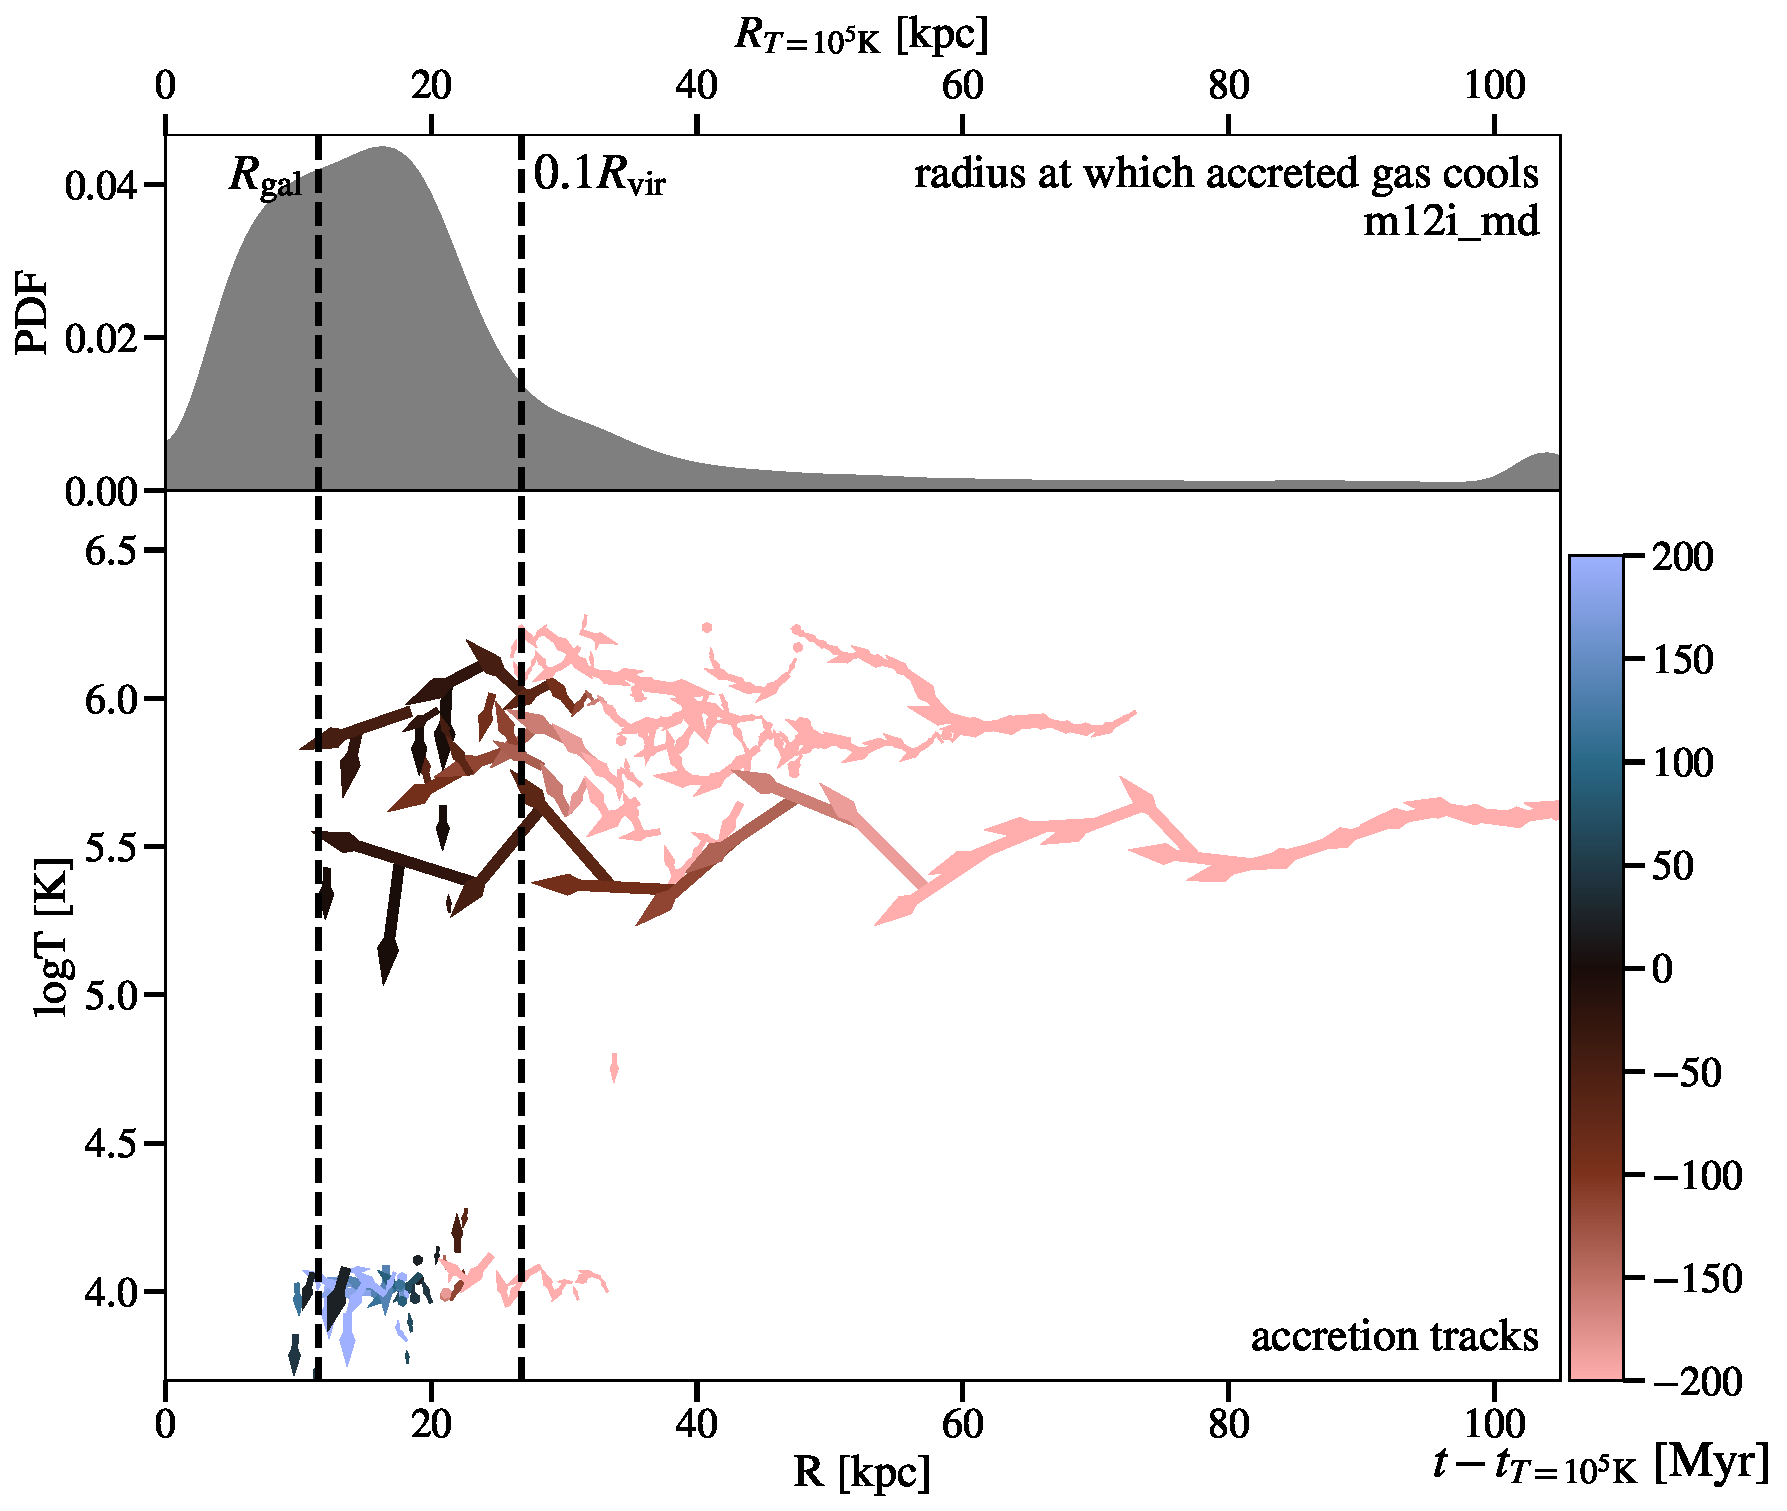
\includegraphics[width=\columnwidth]{figures/tracks/tracks_m12i_md.pdf}
%     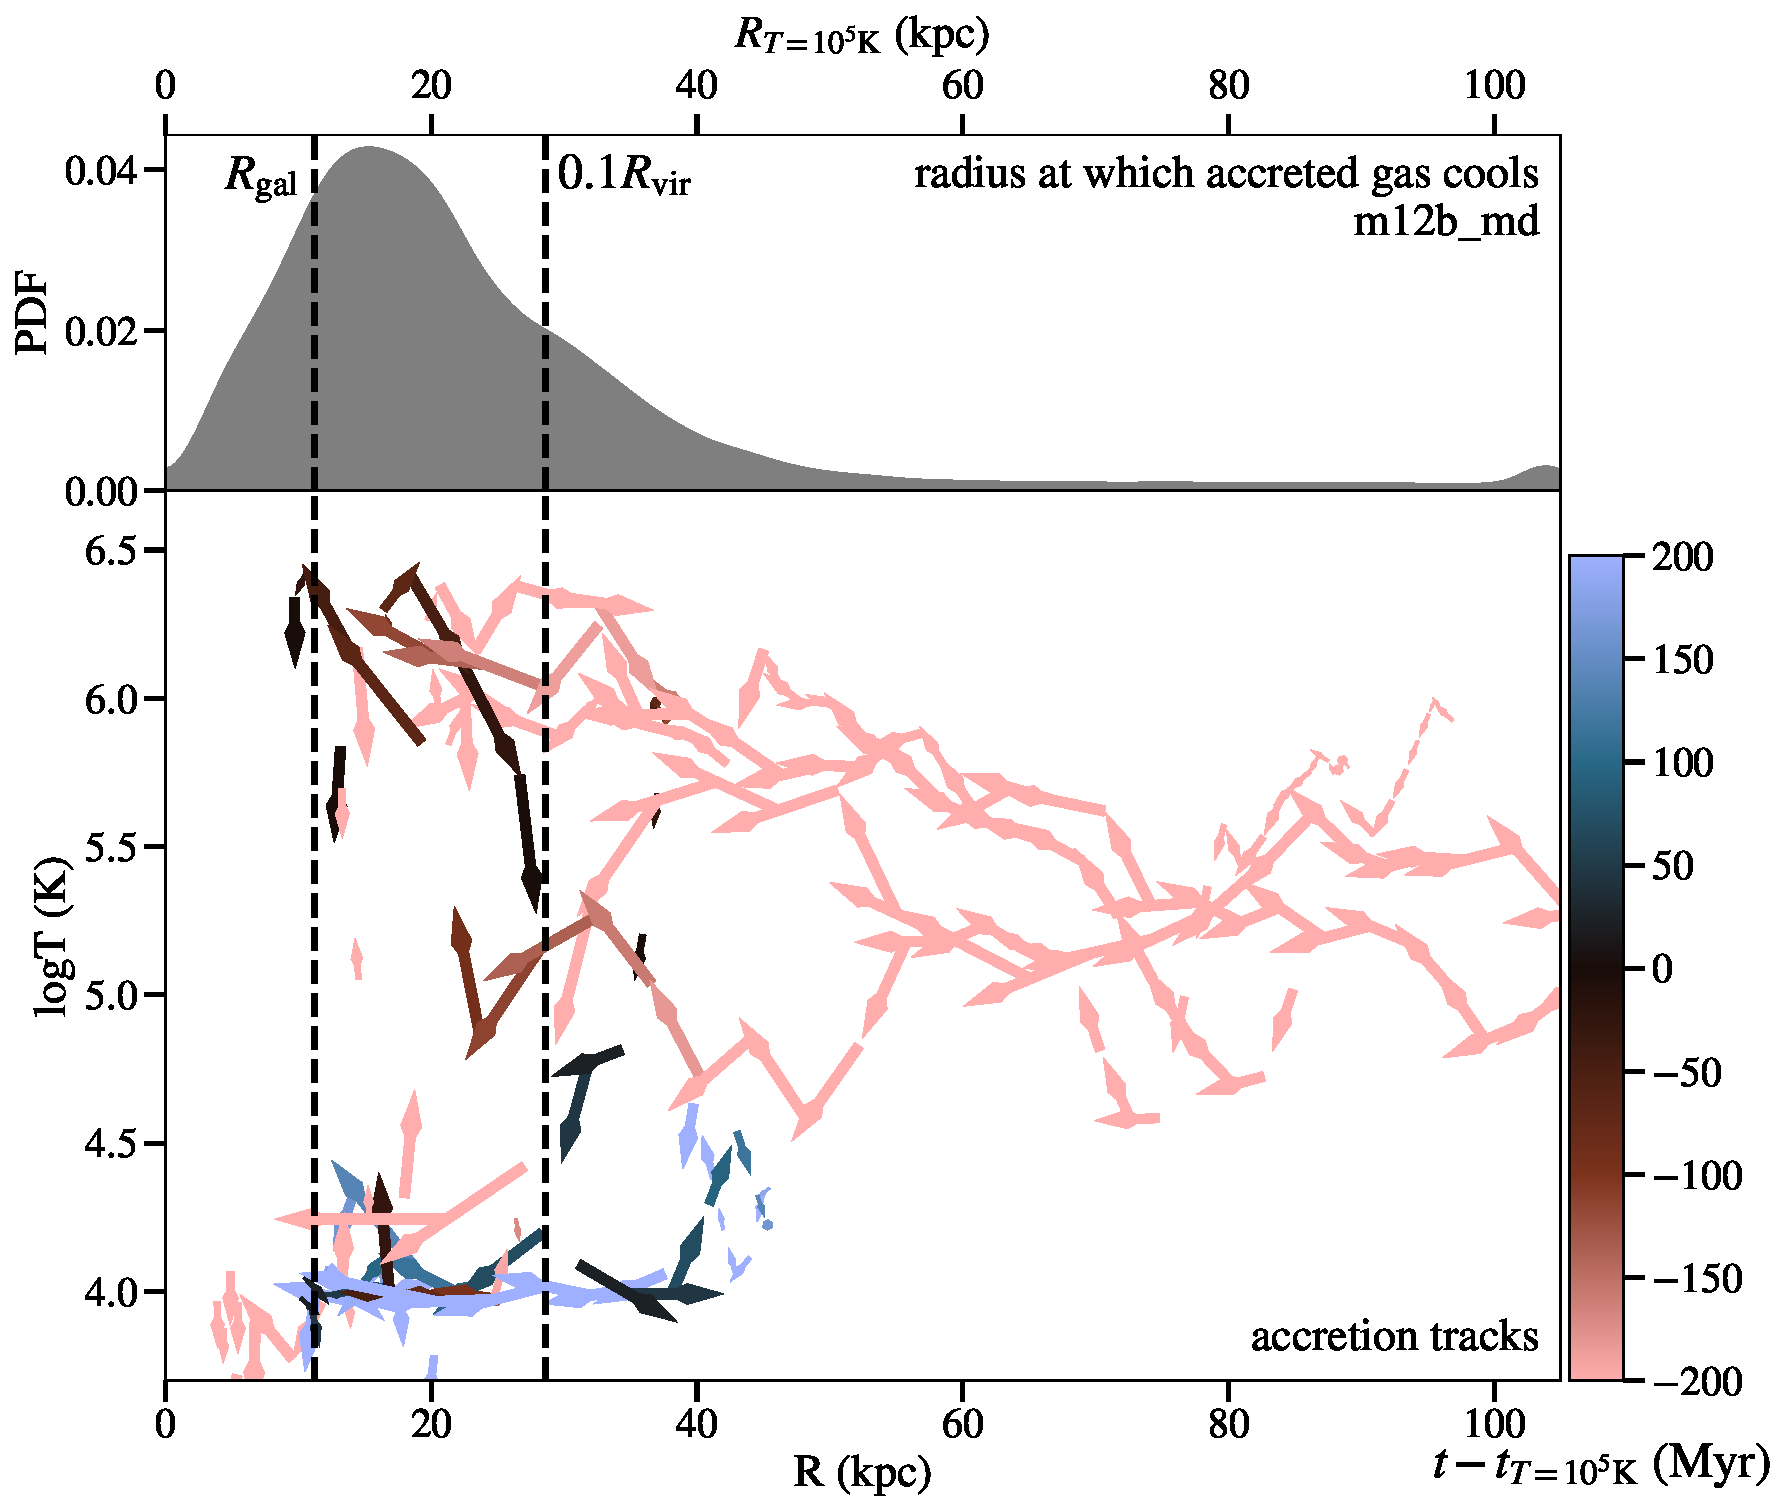
\includegraphics[width=\columnwidth]{figures/tracks/tracks_m12b_md.pdf}
%     \caption{
%     Radial and temperature trends for gas accreting onto two $L^\star$ FIRE halos at $z\approx0$.
%     \textbf{Top panels:} Distribution of $\Rcon$, the radius at which gas particles last cooled below $T=10^5$ K prior to accreting.
%     \textbf{Bottom:} Temperature vs radius tracks for five randomly-selected particles per halo, with color indicating time relative to the time at which gas cools.
%     At $r \gtrsim 0.1 R_{\rm vir}$ accreting gas typically remains hot.
%     }
%     \label{f: T vs R}
% \end{figure*}

% % OBSERVATIONAL COMPARISON
% \begin{figure}
% \centering
% 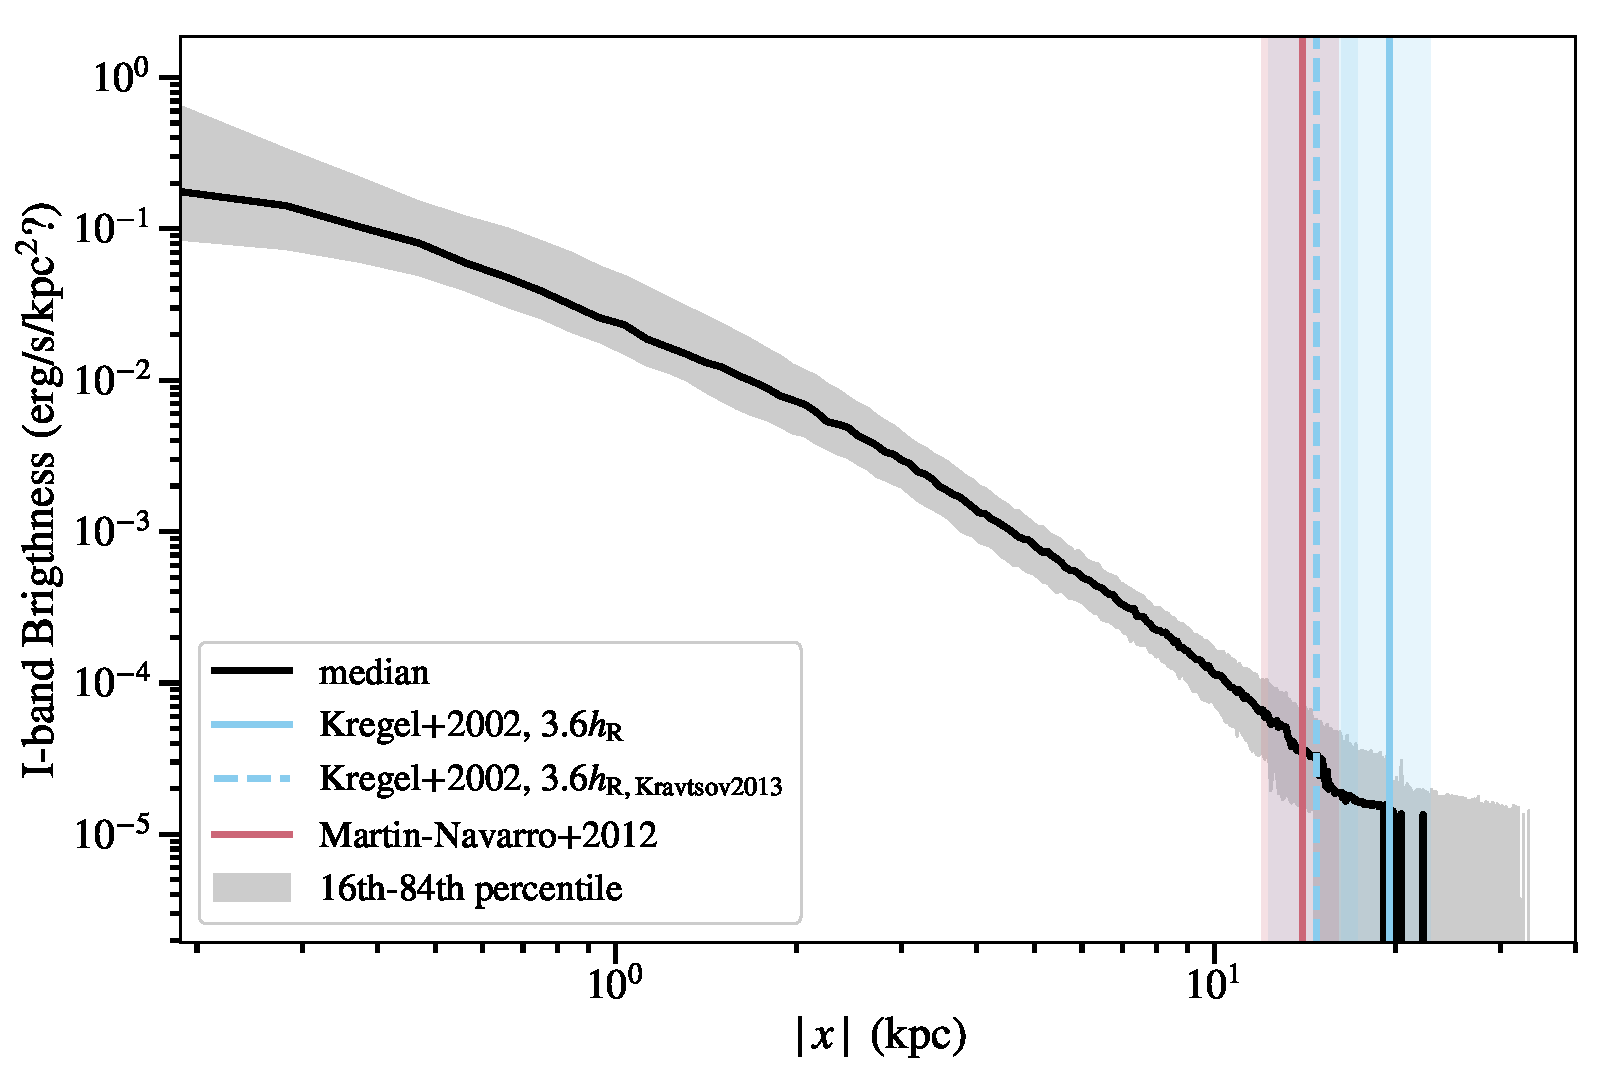
\includegraphics[width=\columnwidth]{figures/brightness_profile.pdf}
% \caption{
% I-band surface brightness profile for an edge-on stellar disk.
% Black line (shaded region) is the median (16th-84th percentile) brightness among pixels 7.5 kpc above/below the disk.
% The disk truncates at $\approx 12$ kpc, as seen by the sharp drop-off in the brightness for the percentiles, consistent with observations.
% \textbf{
% Fill out observations description.
% Put on log-linear axis.
% Cut out inner radii where dust obscuration is likely an issue.
% Maybe cut out entirely and just reference Cameron's paper.
% Reference Shea and Kareem's papers.
% }
% }
% \label{f:stellar_profile}
% \end{figure}

% SPARE FIGURE
% \begin{figure}
%     \centering
%     % \includegraphics{}
%     \caption{
%     \textbf{Spare figure, but maybe
%     cooling emission in X-ray, optical and UV lines vs.\ radius, only from tracked particles
%     }
%     }
%     \label{f: emission}
% \end{figure}

% \section{NOTES FOR AUTHORS}

% \subsection{KEY FOR COAUTHORS}
% \textbf{Bold: Notes for things to implement.} \\
% \textit{Italics: Rough text, needs polishing.} \\
% Normal: Normal text, polished enough to be included in a draft.

% \subsection{OUTSTANDING QUESTIONS/DISCUSSION POINTS}

%  \textbf{Add \texttt{m12z\_md}.}

% \textbf{
% How am I treating 1e4 K gas?
% As radiatively cooling, or in UVB equilibrium?
% }

% \textbf{
% Move Figure~\ref{f: Mdot} to appendix.
% }

% \textbf{
% Cut out Figure~\ref{f: R1e5K}.
% }

% \textbf{
% Move Figure~\ref{f: prevalence vs galaxy properties}.
% }

% \textbf{
% Copy up top panels from Figure~\ref{f: before and after}.
% }

% \textbf{Do all the metal diffusion simulations suffer from the cosmic ray heating bug?}
% Check this. (It's not just for cosmic ray runs.)

% \textbf{T=1e5K is already cooled.}
% Use cautious language about how to phrase the fact that there's cooling before T=1e5K.

% \textbf{Talk about the origin of the gas?}

% \textbf{Kretschmer+2020 might be very disky by measure of V/sigma.}

% \textbf{Make sure Brooks+2009 is included.}

% \textbf{How fast does this deplete the halo?}

% \textbf{
% Feedback-induced accretion may or may not prefer disk formation.
% Increased SFR means increased accretion.
% }

% \textbf{
% Post-starburst galaxies that are restarting star formation may be a test case for disentangling 
% }

% \textbf{Turn off feedback after a given snapshot.}
% This will turn off feedback-induced accretion, but will not turn off rotating cooling flows.

% Cosmological simulations may not have the resolution to induce feedback-induced accretion.

% FIRE MWs have a much wider variation in SFR than the FIRE-2 MWs.
% Esp. m12q and m12v, which weren't rerun.

% \textbf{What are the summary points to frame the paper around, always returning to those?}
% Thin disks are built from rotating cooling flows that collapse directly into a coherent cool disk at the galaxy edge (i.e. they concurrently cool and circularize).
% This is enabled by increased coherence as the gas journeys through the halo.

% \textbf{Add m12z, because it's messy.}
% \textbf{Maybe add thelma.}

% \textbf{Disk observations:
% \url{https://ui.adsabs.harvard.edu/abs/2021MNRAS.506..323T/abstract}
% \url{https://arxiv.org/abs/1207.7072}
% }

% \textbf{
% Caution from Jonathan: in results section of figure 8 esp. be careful about doing interpretatin alongside results.
% }

% \textbf{Add other metrics for diskiness for comparison and to catch people's attention.
% Rd/hd, vrot/sigma.
% }

% \textbf{
% The interpretation of Figure~\ref{f: prevalence} is still kind of confusing.
% How does the aligned accretion fraction relate to the actual fraction of gas accreted via a rotating cooling flow?
% From \S\ref{s: characteristics} we know that the vast majority of gas accretes via a rotating cooling flow.
% However, a naiive assumption of $f_{\rm rotating\,cooling\,flow} \approx \Delta f_{\rm aligned}$ gives $f_{\rm rotating\,cooling\,flow} \le 0.35$.
% This is partially because a cut of $\vert z/R\vert < 0.1$ isn't inclusive enough, but I worry that our readers will get the wrong impression.
% }

% \textbf{
% I don't think we define rotating cooling flows early enough (or clearly enough).
% We should think about where to introduce this concept.
% }
% Abstract?
% Intro?
% Methods?
% Results?

% \textbf{Do we want to compare to the jbar, Mbar, fgas scaling relation from \cite{Pina2021}?}

% Do a loop through and replace Milky-Way-mass with MW mass, defining the earliest usage.

% \textbf{The results could be even stronger if we could test this for one or two more irregular MW-mass galaxies.}
% \textbf{Extend simulation sample to massive galaxies?}
% \textbf{Extend simulation sample to ELVIS galaxies?}

% \textbf{Double-check the definition of t1e5.}
% I need to especially make sure that there's no weird behavior in the following case:
% gas that's cool and within Rgal but insufficiently dense that becomes denser and therefore part of the galaxy.
% This event should *not* be counted as $\tcon$.
% \textit{However}, this should be done after the manuscript is out to collabs.
% If I'm being overly inclusive then fixing that will just strengthen results.
% Check first vs last time cooled.
% Check dependence on galaxy density criterion.
% In some plots, as part of an ancient decision, I'm not plotting recycled material.
% Is that a good choice?

% Is the weirdness with \texttt{m12i\_mhdcv} a general property of MHD sims?
% Leaving it out until I understand this.

% \textbf{Calculate if CR and other halos are undergoing a cooling flow}
% Compare inward velocity to cooling rate.

% % Target audience
% \textbf{
% Who is the target audience?
% }
% My thoughts are\ldots
% At the broadest level anyone who wants to understand the general picture of how disks form.
% Always need both theorists and observers, though a bit more focus on theorists.
% Explaining a galaxy observation using CGM theory.
% People who like interpretable results.

% % Assess the overall message
% \textbf{What points are likely to resonate with the target audience(s)?}
% Imagine sitting down with the target audience.
% What are the most important points you want to convey?
% In particular, what could they really use?
% Think first and foremost of that, and shape accordingly.

% % Review
% Read through the paper with each targeted group in mind.
% Edit accordingly.
% Even better, get a member of the target group to provide feedback.
% At the end, decide on the title and the abstract.

% % Citations
% \textbf{I'm a bit citation-happy right now, what should I trim?}

% % Temporary cooling investigation
% \textbf{Why do some trajectories cool and then reheat?}
% They cool because of perturbations~\citep{Esmerian2020}, but why do they reheat?
% Why is there cool gas visible in the intuition-building plots 100 Myr prior to cooling?

% % How much to include on CR sims
% Pros of including CR-analysis:
% - The physical mechanisms do not require the halo to be a classic virialized hot halo.
% - According to our three characteristics that define quiet accretion, quiet accretion is observed in CR simulations.
% - Quiet accretion is a more interesting concept if we point out its generality.
% - Cameron Trappe also wrote a paper, and one of the main differences is the inclusion of cosmic rays. I'm not sure there's room to do a third entirely separate paper on cosmic ray quiet accretion. Most things will have been covered.
% - As an extension of the previous point, because Cameron wrote the CR paper we can just include a single plot or so and point to his paper for the details of how accretion works.
% Cons:
% - CR halos are regarded as fundamentally different to hydro halos
% - Jonathan's previous work doesn't touch on CR halos.

% % More terminology
% \textbf{In regards to coherence, should we use decoherent, incoherent, or something else?}
% Don't use the term coherence on its own, use dispersion of jz around the average.
% \textbf{Compression heating and radiation cooling, or radiative cooling and compressive heating?}
% Radiative cooling and compression heating.

% % Not overly centered on disk formation
% Are we overly-centered on disk formation?
% Framing of conducive to disk formation might give your listeners the impression that this is the only theory for disk formation.

% % Outer virialized halo effects
% Check the following picture, suggested by James:
% Far enough out in an m11 the inner halo is virialized, and compressive heating can contribute comparably to cooling.
% This would suggest the cooling radius is max( edge of the virialized area, angular momentum radius), potentially true across all halo masses MW and below.
% Can be checked by making an equivalent to Figure~\ref{f: before and after} for an m11.

% % Decreasing halo mass implications
% Do we want to diskuss the conditions under which there could be an early onset of quiet accretion for lower-halo mass halos?

% % Firefly changes
% I need to set up a good preset. Requires changing using options. Can load a preset using the Options class.)
% Change loading screen.
% Include labels for scale.

% % Plots for a future observational paper
% Multi-panel image:
% HI-weighted row,
% OVI?-weighted row,
% T-colored row.
% Before column(s), at column, after column.
% Try mollweide projection.
% Try classic kinematic picture showing blue/red-shift along LOS.

% % Additional visualizations
% Try making a 2D histogram of $\Rcon$ and the angle at which it accretes.

% % Angular momentum reading
% There's still more angular momentum reading to be done, including:
% Cadiou2020; Angular momentum evolution can be predicted from cosmological initial conditions\\
% Filippo's collaborator work: \url{https://ui.adsabs.harvard.edu/abs/2017MNRAS.467..311P/abstract}\\
% Krolewski2019; Alignment between filaments and galaxy spins from the {MaNGA} integral-field survey
% Look at \cite{Bird2019}, which looks at alignment of galaxy disks with filaments.
% Look at \cite{Bird2020}, which seems to be a typical classic disk galaxy paper.
% Maller\&Dekel2002: angular momentum as a function of origin.

% % Angular momentum of accreting gas vs all gas at a given radius
% How does the angular momentum of all gas at a given radius compare to the angular momentum of the accreting gas?
% Check by calculating the inner product between the two?

% % Misaligned or warped disks
% Can quiet accretion produce misaligned or warped disks?
% Tjitske has seen in large scale simulations a misaligned disk being preceeded by a change in halo angular momentum.
% Anna has some plots of this. This might be more present in the ELVIS sims.
% The angular momentum vector of the CGM is in general misaligned with that of the stars in the central galaxy by large angles  30 to 60 degrees (DeFelippis et al. 2020).
% See also Roskar2010.
% Yuan Li finds changing angle of disk due to accretion in her cluster sims.

\section{Introduction}
\label{s: introduction}

% THE THIN DISKS
\begin{figure*}
    \centering
    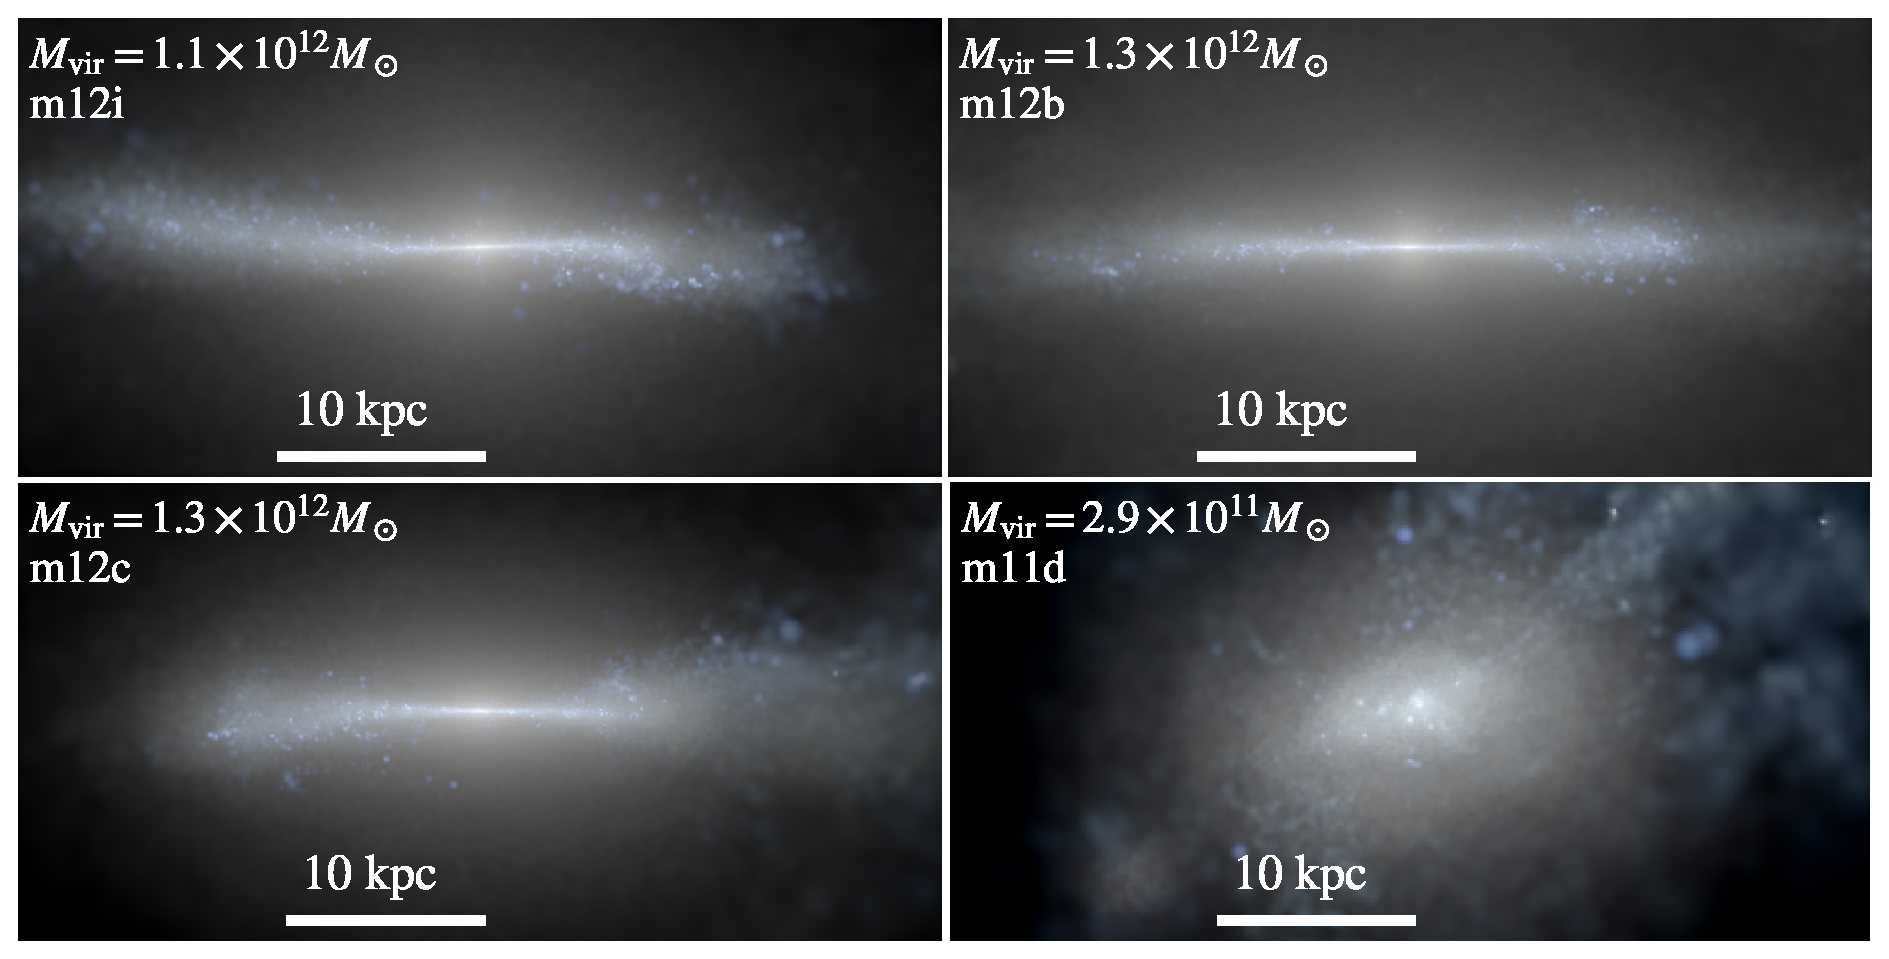
\includegraphics[width=\textwidth]{figures/stars.pdf}
    \caption{
    Mock Hubble images of four $z=0$ galaxies in the FIRE-2 simulations. Halo masses are noted in the panels, together with the fraction of young ($<1$ Gyr) stars which reside in a thin disk.  The Milky-Way-mass galaxies have thin disk morphologies (top, bottom-left), while the lower mass galaxy has an irregular morphology (bottom-right).
    % \textbf{
    % Try changing dynamic range.
    % }
    }
    \label{f: stars}
\end{figure*}

% Basic disk formation idea, and its limitations
Our present picture for the formation of galactic disks can be largely traced to analytic ideas first explored by \citet{fall1980}, where a galaxy's angular momentum is intimately tied to the corresponding properties of its host dark matter halo.
Collapsing structures in an otherwise expanding universe will be spun up by the large-scale matter field \citep{Peebles69};
this can deliver enough angular momentum to allow (at least some) galaxies to have significant angular-momentum support~\citep[e.g.][]{MMW98}. 
Despite this understanding, a full accounting of the origin of disk formation in a cosmological context is incomplete --- the detailed properties of disks formed in cosmological simulations cannot be explained by an understanding of dark matter spin alone~\citep[e.g.][]{GK18}.  

% The puzzle of thin disks
Given what we know about the angular momentum distribution in galactic halos, it is somewhat surprising that so many galaxies are dominated by {\em thin} disks, with small scale heights and vertical velocity dispersions relative to the scale radii and circular speeds $h/R \sim \sigma_z/V_c \sim 0.1$~\citep[][]{Kregel2002, Kregel2002}.
We know, for example, that the angular momentum distribution of dark matter \citep{B01} and gas \citep{Stewart2013,DeFelippis2020} in galactic halos is quite broad.
This means that in order for a tightly-ordered thin disk to emerge the gas must become coherently aligned along a single plane \textit{after} being part of the quasi-spherical extended galactic halo and \textit{before} forming stars.
This suggests that the process by which gas is deposited from the galactic halo into the galaxy, and how this process affects the angular momentum distribution, is an essential aspect of thin disk formation.
 
% Accretion
The process by which gas is deposited into a galaxy from the CGM has been the subject of considerable exploration over the past decade~\citep[e.g.][]{Keres2005, Dekel2006, Keres2009, Angles-Alcazar2017, Martin2019a} with broadly two paths to galaxy fueling identified: hot mode and cold mode.
In the cold-mode case, gas is deposited into the galaxy without ever virializing; this occurs typically in lower mass halos, where the gas cooling time is shorter than the infall time.
% Accretion types - hot
In hot mode accretion, which dominates for massive halos at late times~\citep[e.g.][]{VandeVoort2011, VandeVoort2012a, Joung2012, Murante2012, Nelson2013}, gas first shock-heats to the halo virial temperature, and then radiates its gravitational and thermal energy prior to accreting onto the galaxy.
Our own Milky Way (MW) is one such galaxy for which hot mode accretion is expected to dominate.
As discussed above, we expect the mode of gas delivery, and the precise means by which gas mixes, cools, and accretes should have a substantial baring on the ability to form thin, coherently rotating disks.  

% Cold mode
In cold mode accretion, cool, $T \sim 10^4$ K cosmological filaments travel into the galaxy from the IGM~\cite[e.g.][]{Keres2005, Dekel2006, Keres2009, Martin2019a}, often along with embedded satellite galaxies~\citep[e.g.][]{Hafen2019, Esmerian2020}.
This mode is expected to dominate the mass inflow rate at high-redshift \citep[$z\gtrsim2$; e.g.][]{Keres2009a, Dekel2009, Huscher2020}.
It is unclear however if the cool filaments remain intact down to the galaxy, or rather heat up and dissolve into the surrounding hot phase~\citep[e.g.][]{Nelson2016, Mandelker2016, Mandelker2018, Mandelker2020a}, in which case hot accretion onto the galaxy would also be important at high redshift.
While cool halo inflow of this kind typically contains more specific angular momentum (in total) than either hot gas or dark matter~\citep{Stewart2017}, the tendency for such gas to reach the galactic region prior to mixing may hinder the ability to develop a thin, coherently aligned structure prior to star formation.
The fact that thin disk galaxies are common only among fairly massive systems $L \sim 0.1 L_\star - L_\star$ at lower redshift~\citep[e.g.][]{Kranz2003, Kassin2006, Bizyaev2021,Kassin+12,Simons+15,Simons+17}, is roughly consistent with the idea that cold-mode delivery is not conducive to thin disk formation.
% Hot mode

An alternative possibility is that hot mode accretion, believed to dominate in more massive halos, is conducive to disk formation. This depends on the specific mechanics of this accretion mode, and on whether the hot gas manages to cool and accrete rather than being reheated by galactic feedback processes.
%The present work focuses on the possibility that thin disks are fed by the \textit{hot accretion mode}, motivated by the recent analysis of the FIRE simulations \citep{Hopkins2018} performed by \cite{Stern2021}, which identified a strong relation between disk formation and CGM virialization (i.e., the formation of a virialized `hot halo', a necessary condition for hot-mode accretion).
% In more massive halos, where hot-mode accretion is believed to dominate, 
% Despite a large body of research, there is yet no consensus on these questions.
One possible subset of hot-mode accretion is instability-driven accretion, wherein gas precipitates out of the hot halo due to thermal instabilities, forming cool clouds which lose buoyancy and accrete onto the galaxy~\citep[e.g.][]{Maller2004, Mccourt2012, Voit2015, Armillotta2016, Gronke2019a, Voit2021}.
% Quiet accretion
Alternatively, radiative cooling in the hot CGM can cause the entire hot phase to flow inward.
In this latter scenario, the inward flow occurs at a rate where compression heating of the hot phase roughly balances radiative losses, so the hot gas roughly retains its temperature.
This type of hot accretion has been termed a `cooling flow' in the context of galaxy cluster studies~\citep[][see \citealt{McNamara2007} for a review]{Mathews1978, Cowie1980, Fabian1984, Balbus1988, Bertschinger1989}. 
\cite{Stern2019, Stern2020} recently revisited cooling flows in the context of galaxy-scale halos, and highlighted the interplay between angular momentum and thermodynamics in these solutions. They found that hot, subsonic cooling flows can smoothly accrete onto a disk (and are thus potentially conducive to  the formation of thin disks) only if the flow becomes angular momentum supported prior to going through a sonic point. 
Otherwise, the inflow turns supersonic and likely goes through a (radiative) shock upon accretion
(see \citealt{Stern2020}, especially figs. 2 and 7). In this paper we demonstrate that cooling flows which satisfy this condition are the primary mode of gas accretion onto disky Milky Way-mass galaxies at $z \sim 0$ in the FIRE cosmological simulations \citep{Hopkins2018}, thus suggesting that such `rotating cooling flows' may be a necessary condition for thin star-forming disks. 


% . Our analysis supplements and is motivated by the results of \citep{Stern2021}, which identified in FIRE a strong relation between disk formation and virialization of the CGM\footnote{CGM virialization has also been referred to as `hot halo formation'.}, where the latter is a necessary condition for the hot accretion mode. 
% Quiet accretion
% using steady-state calculations and idealized hydrodynamic simulations. They demonstrated that a necessary condition for a hot inflow down to the galaxy scale is that the sonic point of the solution is smaller than the circularization radius (the radius where angular momentum support can halt the inflow). This condition roughly translates to a hot gas cooling time at $\approx0.1\Rvir$ larger than the local free-fall time. We demonstrate below that this condition also holds under the more realistic conditions implemented in cosmological simulations. 

From an observational perspective, cooling flows are difficult to observe for galaxies beyond $z\sim0$~\citep{Putman2012}.
This follows since cool CGM gas is typically more accessible to observations than the hot CGM, but in cooling flows the accreting gas becomes cool only when it has no significant spatial or kinematic offset from the galaxy.
\citeauthor{Putman2012} thus called this accretion mode ``quiet accretion''. 
% This quiet accretion could explain observations at higher redshifts that show substantial SFRs and outflows with little, if any, evidence for accretion (e.g., Erb 2008, Steidel et al. 2010, Shapley 2011)~\citep{Putman2012}.
Consistent with quiet accretion, some observational studies argue that the accretion implied by cool gas observe in the halos of massive disks is insufficient to sustain star formation \citep[e.g.][]{Sancisi2008, Binney+09}, while others detect ionized, inflowing gas at the galaxy-halo interface~\citep{Zheng2017}. Furthermore, X-ray absorption studies suggest that hot gas in the inner CGM of the Milky-Way is rotating \citep{Hodges-Kluck2016}, consistent with a rotating cooling flow. 

% Cosmological simulations
Modern cosmological simulations provide a means to understand the characteristics, prevalence, and mechanics of different accretion modes.
These simulations include a combination of cosmological environment and galactic physics, which has allowed simulators to investigate accretion while accounting for both its cosmological nature and its interaction with galaxies and their CGM~\citep[e.g.][]{Oppenheimer2010, Stewart2011, Fernandez2012, Ford2014, Angles-Alcazar2017, Hafen2019, Hafen2020, Ho2019, Rottgers2020, Trapp2021}.
Of special note are ``zoom-in'' simulations that focus on resolving a single halo and its environment, enabling high resolution while preserving cosmological structure~\citep[e.g.][]{Katz1993, Wang2015, Agertz2020}.
Among these the FIRE simulations~\citep{Hopkins2014, Hopkins2018b}\footnote{\url{https://fire.northwestern.edu/}} are a set of zoom-in simulations that resolve stellar feedback on the scale of giant molecular clouds in the ISM, producing winds that naturally expand into the CGM and interact with accreting gas~\citep{Muratov2015, Muratov2017, Hafen2019, Hafen2020}.
The resultant galaxies are broadly consistent with the stellar mass-halo mass relation~\citep{Hopkins2017}, the mass-metallicity relation~\citep{Ma2016a}, satellite galaxy populations~\citep{Wetzel2016, Garrison-Kimmel2019a}, and can have thin-disks consistent with Milky Way-like galaxies~\citep{Garrison-Kimmel2018, El-Badry2018}.

This paper is part of a series of FIRE papers exploring the relation between the formation of thin disks and the properties of the CGM \citep{Stern2021, Yu21, Gurvich_in_prep, Byrne_in_prep}. The analysis here follows \cite{Stern2021}  who showed that disk settling in FIRE is closely connected to the formation of a virialized and stable hot CGM, which is a necessary condition for the onset of hot accretion. 
We also utilize the FIRE simulations to explore the mechanics of rotating cooling flows near the disk-halo interface where angular momentum support is substantial,  thus going beyond 1D steady-state solutions developed in classic ICM studies~\citep[e.g.][]{Cowie1980}, and extending the idealized 3D simulations in \cite{Stern2020} to a more realistic cosmological setting. 
% Our simulations include stellar feedback processes but no AGN feedback processes, this result suggests that cooling flows may be  prevalent in galaxies where AGN feedback is weak or absent, and that cooling flows can be used as a benchmark for AGN feedback studies. 

% This paper
This paper is structured as follows. 
In \S\ref{s: methods} we describe our sample of FIRE simulations and the sample of accreting particles selected from the simulations.
In \S\ref{s: characteristics} we analyze the characteristics and mechanics of gas accretion onto $z\sim0$ galaxies in FIRE, and their relation to thin disk morphology in the central galaxy. We discuss our results in \S\ref{s: discussion} and conclude in \S\ref{s: conclusions}.

\section{Methods}
\label{s: methods}

\subsection{Simulations}
\label{s: methods -- simulations}

\begin{table*}
\caption{Simulation parameters.}
\begin{tabular}{cccccccc}
\hline
Name  &  $f_{\rm thin\,disk,\,recent}$  & $M_{\rm vir}$  &  $M_\star$  &  $R_{\textrm{vir}}$  &  $\Delta f_{\rm aligned}$  &  Physics  &  Reference  \\
  &   & $M_\odot$  & $M_\odot$  &  kpc  &  &  &  \\
 \hline
m12i  &  0.83  &  $1.1\times10^{12}$  &  $7.3\times10^{10}$  &  268  &  0.34  &  hydro+  &  ?    \\
m12b  &  0.8  &   $1.3\times10^{12}$  &  $1.0\times10^{11}$  &  286  &  0.32  &  hydro+  &  ?    \\
m12c  &  0.72  &   $1.3\times10^{12}$  &  $6.8\times10^{10}$  &  283  &  0.2  &  hydro+  &  ?    \\
m12f  &  0.72  &   $1.5\times10^{12}$  &  $9.7\times10^{10}$  &  302  &  0.21  &  hydro+  &  ?    \\
m12i\_core  &    0.79  &  $1.1\times10^{12}$  &  $8.0\times10^{10}$  &  274  &  0.29  &  no MD  &  ? \\m12m  &  0.37  &  $1.5\times10^{12}$  &  $1.4\times10^{11}$  &  298  &  0.28  &  no MD  &  ?    \\
 m12w  &  0.33  &  $9.5\times10^{11}$  &  $6.5\times10^{10}$  &  253  &  0.15  &  hydro+  &  ?    \\
m11h  &  0.24  &  $1.8\times10^{11}$  &  $3.9\times10^{9}$  &  146  &  0.051  &  hydro+  &  ?    \\
m12r  &  0.16  &   $1.0\times10^{12}$  &  $2.4\times10^{10}$  &  257  &  0.13  &  hydro+  &  ?    \\
m11e  &  0.05  &   $1.5\times10^{11}$  &  $1.6\times10^{9}$  &  136  &  0.049  &  hydro+  &  ?    \\
m11i  &  0.023  &  $7.0\times10^{10}$  &  $1.0\times10^{9}$  &  106  &  0.02  &  hydro+  &  ?    \\
m11a  &  0.018  &  $4.1\times10^{10}$  &  $1.3\times10^{8}$  &  90.3  &  -0.022  &  no MD  &  ?    \\
m11c  &  0.015  &  $1.4\times10^{11}$  &  $9.5\times10^{8}$  &  137  &  0.00072  &  no MD  &  ?    \\
m11d  &  0.0097  & $2.9\times10^{11}$  &  $4.9\times10^{9}$  &  169  &  0.0067  &  hydro+  &  ?    \\
m11q  &  0.0058  &  $1.5\times10^{11}$  &  $7.4\times10^{8}$  &  138  &  -0.012  &  hydro+  &  ?    \\
% m12i\_CR  &  0.81  &  4  &  9.7  &  $1.1\times10^{12}$  &  $6.5\times10^{10}$  &  270  &  0.27  &  CR+  &  ?    \\
   \\
\end{tabular}
\\
\begin{flushleft}
Properties at $z=0$ of the sample of FIRE galaxies analyzed in this work. The value of
$f_{\rm thin\,disk,\,recent}$ is the fraction of stars formed in the last Gyr prior to $z=0$ that are in a thin disk configuration ($j/j_c(E) > 0.8$; e.g. \citealt{Yu2021}).
% $M_{\rm vir}$ is the total mass contained within $R_{\rm vir}$ and $M_\star$ is the total stellar mass contained within the galaxy radius~(\S\ref{s: methods -- analysis}). 
The value of $\Delta f_{\rm aligned}$ is a measure of the relation between cooling and circularization in accreted gas (\S\ref{s: characteristics -- aligns}).
The ``hydro+'' simulations include fiducial FIRE physics, while the ``no MD'' simulations exclude a prescription for subgrid metal diffusion.
% The ``CR+'' simulation includes cosmic rays.
The references in the final column are:
\textbf{TBD.}
% A: \cite{Hopkins2017},
% B: \cite{Chan2018},
% C: \cite{Wetzel2016},
% D: \cite{Garrison-Kimmel2017a},
% E: \cite{El-Badry2017},
% F: \cite{Garrison-Kimmel2018},
% G: Samuel et al., in prep.
% \textbf{Why are my disk metrics lower than 10? (And in one case nan.)}
% \textbf{I may be calculating not the half height, but the h85 height.}
% \textbf{Do V/sigma only for gas? It's *much* higher.}
% \textbf{Show R/h only for the stars we identify as thin disk.}
% \textbf{Add Alex's vector to total ratio?}
% \textbf{Rerun CR halo.}
% \textbf{Say the values in the text, don't add them here. Ref Anna's paper.}
\end{flushleft}
\label{table: simulations_used}
\end{table*}

% % Comparable samples
% \textit{
% \cite{Garrison-Kimmel2018} perform a related analysis using simulations from the ELVIS suite and \texttt{m12i\_md}, \texttt{m12f\_md}, \texttt{m12b\_md}, \texttt{m12m\_md}, \texttt{m12c\_md}, \texttt{m12w\_md}, \texttt{m12q}, \texttt{m12z\_md}.
% \cite{Yu2021} perform a related analysis using simulations from the ELVIS suite and \texttt{m12i\_md}, \texttt{m12f\_md}, \texttt{m12b\_md}, \texttt{m12m\_md}, \texttt{m12c\_md}, and \texttt{m12w\_md}.
% Gurvich et al., in prep, perform a related analysis using simulations \texttt{m12i\_md}, \texttt{m12f\_md}, and \texttt{m12b\_md}.
% }

% FIRE simulations
We analyze the hydrodynamical cosmological zoom-in simulations produced as part of the FIRE project~\citep{Hopkins2014}.
The simulation sample, listed in Table~\ref{table: simulations_used}, were run with the FIRE-2 version~\citep{Hopkins2018b} of the gravity and hydrodynamics code \textsc{GIZMO}\footnote{\url{http://www.tapir.caltech.edu/\~phopkins/Site/GIZMO.html}}~\citep{Hopkins2015}.
The simulations were produced using the meshless finite-mass (``MFM'') mode of \textsc{GIZMO}, a Lagrangian method with no inter-element mass flux.
This enables use to track the history of each resolution element.
The full details of simulations produced with the FIRE-2 code are available in~\cite{Hopkins2018b}.
The FIRE simulations include detailed prescriptions for star formation and stellar feedback.
Each star particle contributes to the simulation momentum from radiation pressure; energy, momentum, mass, and metals from Type Ia and II supernovae and stellar winds; and photo-ionization and photo-electric heating.
Star formation is limited to self-gravitating, molecular, self-shielding gas with a density of at least $n_{\rm SF} = 1000$ cm$^{-3}$.
In the simulations and throughout our analysis we use a standard flat $\Lambda$CDM cosmology with $\Omega_{\rm m }\approx 0.32$, $\Omega_{\Lambda}=1-\Omega_{\rm m}$, $\Omega_{\rm b} \approx 0.049$, and $H_{0} \approx 67$ km s$^{-1}$ Mpc$^{-1}$~\citep[e.g.,][]{PlanckCollaboration2018}.

% Metal diffusion

% The metal distribution in the CGM affects cooling processes and therefore the treatment of metal diffusion is important for resolving substructure and small clouds
% Failure to resolve substructure may result in failure to produce instability-driven accretion.
% More diffusive metal diffusion typically produces fewer cool clouds, with possible exceptions for stripping processes, and many current prescriptions for metal diffusion may under-resolve metal diffusion~\citep[e.g.][]{rennehan2019, rennehan2021}.
% Therefore if cool cloud substructure is not present with under-resolved metal diffusion, as may be the case in our simulations, we do not expect it to arise with an alternative metal diffusion treatment.
% Further, a subset of our simulations do not include metal diffusion, providing a more conservative test of the presence of instability-driven accretion.

% Figure 1
Figure~\ref{f: stars} shows edge-on mock Hubble images (with no dust attenuation) for the $z=0$ snapshots of four of our simulated galaxies. The top and bottom-left panels show three MW-mass galaxies (\texttt{m12i}, \texttt{m12b}, and \texttt{m12c}) while the bottom-right panel shows a $M_\star \sim 10^9 M_\odot$ galaxy, \texttt{m11q}.
As noted in previous studies \cite{?} MW-mass galaxies in FIRE typically have thin disk morphologies, while lower mass galaxies show a thick disk / irregular morphology. We quantify this trend using $f_{\rm thin\,disk,\,recent}$, defined as the fraction of stars with age $<1$ Gyr (at $z=0$) that have $j_z/j_c(E) > 0.8$, where $j_z$ is the specific angular momentum in the $z$ direction and $j_c(E)$ is the angular momentum the star would have if it had the same energy but was in a circular orbit. The $z$ axis is defined as the direction of the total angular momentum vector of stars inside the galaxy.  This definition of the thin disk is the same definition used in~\cite{Yu2021}. Values of $f_{\rm thin\,disk,\,recent}>0.7$ correspond to height to size ratios $h/R\sim0.1$ and rotation to dispersion ratios $v_\phi/\sigma\sim10$, and correlate strongly with the observed thin disk fraction in the r band (appendix \ref{s: appendix-sloan thin disk fraction}). The values of $f_{\rm thin\,disk,\,recent}$ are noted in Fig.~\ref{f: stars} and listed in Table~\ref{table: simulations_used}. 
% We will use this subsample of simulated galaxies throughout much of our analysis.
% Most of our MW-mass galaxies have high young thin disk fractions, while our lower mass galaxies have thick-disk, irregular, or spherical morphologies.


\subsection{Analysis}
\label{s: methods -- analysis}

% How we select the particles
For each galaxy we use the particle tracking method described in \cite{Hafen2019, Hafen2020} to select all resolution elements (particles) that have accreted onto the central galaxy during the last Gyr prior to $z=0$. To select such particles, we require that they are (1) within the galaxy radius $R_{\rm gal}$ at $z=0$, either in stars or in gas with density  $n_{\rm H} > 0.13$ cm$^{-3}$, and (2) within the CGM (gas at $0.1 - 1 \Rvir$) at some time in the last Gyr of the simulation. Throughout the paper we use $r$ for the 3D distance and $R$ for the cylindrical radius. 
We define $R_{\rm gal} = 4 R_{\star,0.5}$ following \cite{Hafen2019, Hafen2020}.
For each selected particle we retrieve the full history of the particle (including temperature, density, and metallicity). 
% Handling duplicate IDS
We discard a small fraction ($<2\%$) of the particles since over time their mass increases by a factor of over two due to mass deposition by stellar feedback. These particles pose a problem for our tracking method because the history of the additional mass is not recorded.

% Definition of t1e5 and calculating it
A key time for our analysis is the last time a particle cools prior to entering the galaxy. For a given particle, we define this time as:
\begin{equation}
    \tcon \equiv t \bigg( {\rm last\,snapshot\,outside\,galaxy\,with\,}T>10^5\,{\rm K} \bigg) ~,
\label{e: tcon}
\end{equation}
i.e., the last snapshot the particle was hot prior to entering the galaxy (according to the galaxy definition above). For gas that cools as it accretes, $\tcon$ occurs as the gas passes through the galaxy-halo interface. Below we analyze the statistical properties of all accreting particles as a function of time relative to their cooling time ($t-\tcon$).
% When selecting values in the simulation corresponding to $\tcon$ we use the last snapshot an accreted particle had $T > 10^5$ K, i.e. the snapshot immediately before the transition.
% For some visualization purposes we interpolate between the snapshot prior to $T = 10^5$ K and the snapshot after $T = 10^5$ K and set $\tcon$ to the interpolated value.
% This is a subtle change that does not affect our results.
% Note that heating within the ISM to $T > 10^5$ K does not affect $\tcon$.
% Because our sample of tracked particles focuses on recently accreted particles this is expected to be a small population that will not contaminate our analysis.
% This is confirmed a posteriori in Figure~\ref{f: theta vs t}, where gas is not preferentially oriented in a disky ISM prior to $\tcon$.

\section{Results}
\label{s: results}

% \subsection{How do disk galaxies accrete?}
\label{s: characteristics}

% INTUITIVE OVERVIEW
\begin{figure*}
    \centering
    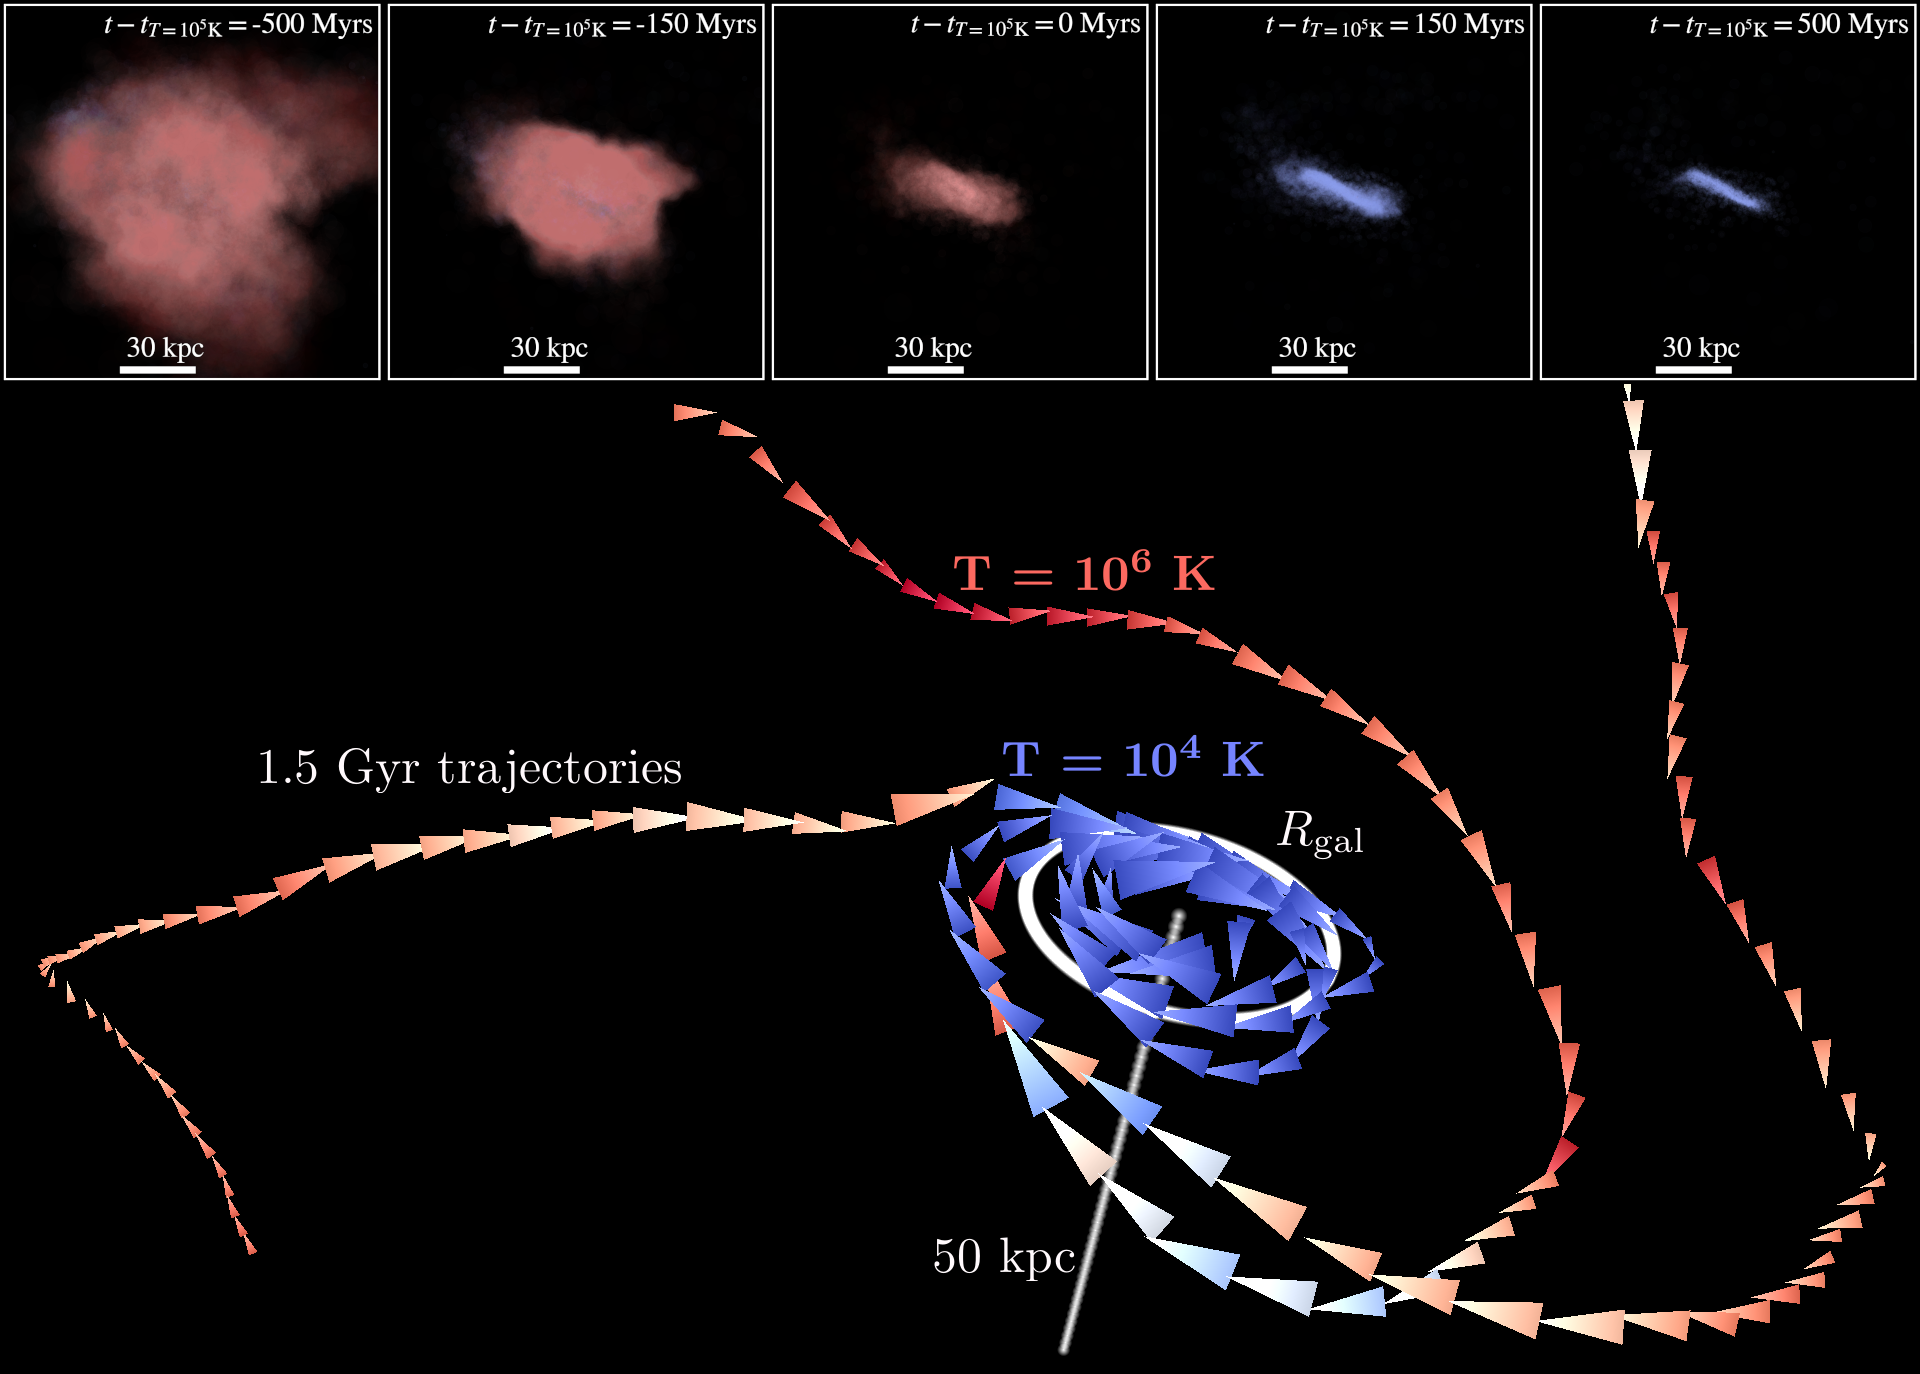
\includegraphics[width=\textwidth]{figures/illustrative_tracks/illustrative_tracks.png}
    \caption{
Gas accretion onto a Milky-Way-mass disk galaxy in FIRE, \texttt{m12i}, near $z\approx0$.
\textbf{Top and right panels:}
Temperature and spatial evolution of accreting gas with respect to $\tcon$, defined as the last time at which the gas cools below $10^5$ K prior to accreting onto the galaxy. 
Red, white, and blue indicates $T=10^6$ K, $10^5$ K, and $10^4$ K respectively. 
\textbf{Bottom-left panel:}
Three representative trajectories for accreting gas elements.
The panels show that accretion is hot ($\approx 10^6$ K) and contracts quasi-spherically at early times relative to the cooling time. At the time of cooling the geometry of accreting gas transitions from a quasi-spherical distribution at $t-\tcon < -150$ Myr to a cool disk at $t-\tcon > 150$ Myr.
% \textbf{Consider adding shape of disk to help frame shape size.}
    }
    \label{f: overview}
\end{figure*}

% Summary picture description
To characterize gas accretion we analyze the central galaxy and its CGM from $z=0$ to one Gyr prior.
Figure~\ref{f: overview} shows a visual overview of how gas accretes onto a MW-mass disk galaxy. 
The top and right panels plot the temperature and spatial evolution of accreting gas versus $t-\tcon$, while the bottom-left panel plots three representative trajectories for accreting gas elements. 
Red, white, and blue indicates $T=10^6$ K, $10^5$ K, and $10^4$ K, respectively. The figure shows that at early times relative to cooling ($t-\tcon<-150$ Myr) the accretion is hot ($\approx10^6$ K) and contracts quasi-spherically. Then, around the time of cooling the geometry of accreting gas transitions from quasi-spherical at $t - \tcon=-150$ Myr to a cool disk at $t - \tcon=+ 150$ Myr. A quantitative analysis of this transition follows in sections \ref{s: characteristics -- inflowing gas phase}--\ref{s: mechanics -- energy balance}.

\subsection{Gas inflow is hot through the CGM}
\label{s: characteristics -- inflowing gas phase}

Figure~\ref{f: before and after A} plots various characteristics of accreting gas on the \texttt{m12i} thin disk galaxy, as a function of time relative to the accretion's last cooling time ($t - \tcon$).
In each panel solid lines and shaded regions mark the medians and 16th to 84th percentile ranges of all particles accreted within $0.5-1$ Gyr prior to $z=0$. The lower limit on the time range applied in this figure is to ensure that particles are present for most of the time displayed after $\tcon$. In the temperature panel (A) we exclude from the distribution particles which converted into stars. 

Panel (A) demonstrates that during the 500 Myr prior to cooling, the inflow is predominantly hot ($\gtrsim 10^5$ K), with a median temperature of $4-8\cdot10^5$ K similar to the halo virial temperature of $\Tvir(z=0)=6.5\cdot10^5$ K. During this time prior to cooling the accreting gas is inflowing toward the galaxy (panel B), from a median $r=55$ kpc at $t-\tcon=-500$ Myr, to a median $r\approx18\,{\rm kpc}\approx1.4 R_{\rm gal}$ kpc at $t=\tcon$. The characteristic inflow velocity of $v_r \approx-70$ km s$^{-1}$ (Panel D) is substantially lower than the circular velocity of $170-200$ km s$^{-1}$, indicating significant pressure support in the accreting gas of $1-(v_r/v_c)^2\approx85\%$. This radial velocity is also smaller than the median sound speed of $100-130$ km s$^{-1}$, indicating a subsonic flow. 


A similar hot inflow is seen in other thin disk galaxies in our sample (appendix~\ref{s: appendix-lowmass}). Thus, accretion from the CGM onto $z=0$ thin disks in FIRE is dominated by the inflow of hot, virial temperature gas. We show below that this accretion flow corresponds to a `cooling flow', similar to the classical solution envisioned for the ICM (e.g., \citealt{Mathews1978}).  Also, we emphasize that this hot accretion mode, in which the entire hot phase inflows, is qualitatively different from `precipitation' in which gas clumps cool at halo scales, lose buoyancy and subsequently accrete (e.g.~\citealt{Maller2004,Voit2017}). The dominance of hot accretion over precipitation in MW-like galaxies simulated in FIRE has previously been noted by \cite{Esmerian2020}. 





% MECHANICS OF QUIET ACCRETION
\begin{figure*}
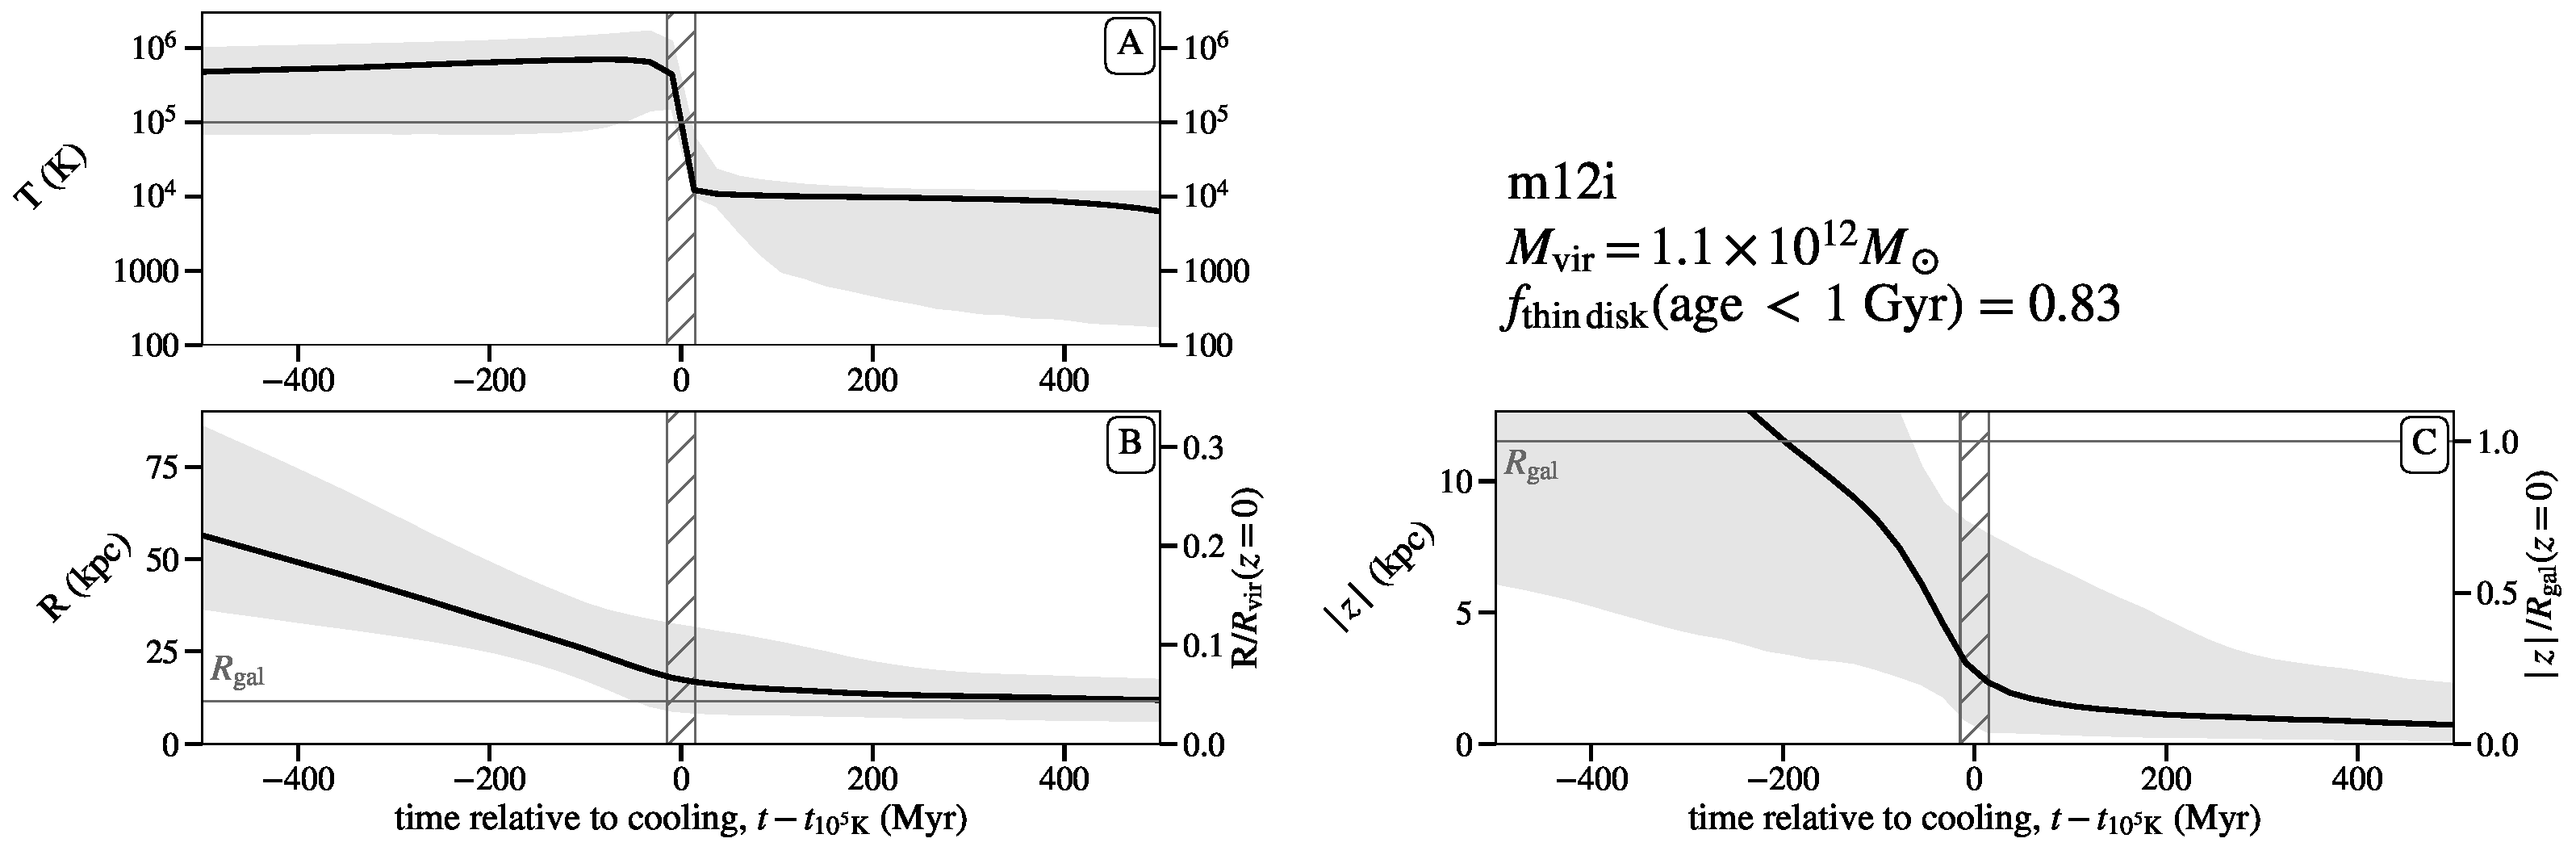
\includegraphics[width=\textwidth]{figures/before_and_after/before_and_after_characteristics_m12i_md.pdf}
\caption{
Properties of gas accretion onto a $z\sim0$ thin disk galaxy in FIRE, versus time relative to the final cooling time ($t - \tcon$).
In each panel solid lines and shaded regions mark the medians and 16th to 84th percentile ranges of all particles accreted within 1 Gyr prior to $z=0$. 
\textbf{A:}
Temperature. During the 500 Myr prior to cooling, the inflow is predominantly hot ($\gtrsim 10^5$ K), with a median temperature approaching $\Tvir\approx10^6$ K. At $t = \tcon$ the gas cools (by definition), and achieves ISM temperatures or forms stars at later times. 
\textbf{B:}
3D distance from halo center. Cooling occurs at $10-30$ kpc, corresponding to $0.7-2.5\,R_{\rm gal}$. Prior to cooling the gas forms an inflow while after cooling the inflow stalls.
\textbf{C:}
Absolute height from the disk plane.
Most of the gas collapses into a disk upon cooling, with a median $\vert z \vert \approx 2$ kpc at $t=\tcon$.
\textbf{D:}
Velocity components of accretion (colored lines and band), relative to circular velocity at the median radius (dash-dotted line). The gas reaches full rotational support upon cooling.
\textbf{E:}
Fraction of gas converted into stars. Star formation starts after cooling, at a rate of $\sim10\%$ per $100$ Myr. 
}
\label{f: before and after A}
\end{figure*}


\subsection{Accretion cools and stalls at the galaxy-halo interface}
\label{s: characteristics -- cools}

Panel (A) in Fig.~\ref{f: before and after A} demonstrates that at $t = \tcon$ the temperature drops from $\sim10^6$ K to $\sim10^4$ K,  as expected from the definition of $\tcon$ (eqn.~\ref{e: tcon}). Panel (B) shows that this cooling occurs just outside the galaxy, at $r(\tcon) \approx 10-30$ kpc, equivalent to $\approx0.7 - 2.5 R_{\rm gal}$\footnote{Note that gas can have $r(\tcon) < R_{\rm gal}$ if it is under-dense relative to the galaxy when it crosses $R_{\rm gal}$ ($n_{\rm H} < 0.13$ cm$^{-3}$), see section \ref{s: methods -- analysis}.}. Less than $10\%$ of particles cool beyond $\sim 40$ kpc. After $\tcon$ the temperature further drops to ISM temperatures of $100-10^4$ K and stars start to form at a rate of $\approx10\%$ per $100$ Myr (panel E), roughly equal to the average rate in the galaxy ISM. 

Panel (D) in Fig.~\ref{f: before and after A} demonstrates that cooling at the galaxy scale is further associated with a change in accretion kinematics. The radial inflow velocity $\vert v_r \vert $ starts decelerating $\approx40$ Myr prior to cooling, and almost completely stalls ($\lesssim10$ km s$^{-1}$) after cooling. This stalling is associated with $v_\phi$ reaching $v_c$, indicating a transition from pressure-support in the hot CGM to rotational support in the cool ISM. Note that deceleration prior to accretion is possible due to the subsonic nature of the hot flow. Similar results are seen for accretion onto other thin-disk galaxies in our sample (appendix \ref{s: appendix-lowmass}). Thus, the majority of accretion onto $z\sim0$ thin disk galaxies in FIRE is a hot inflow which cools and stalls just outside the galaxy. 


% % COOLS AT DISK INTERFACE
% \begin{figure*}
%     \centering
%     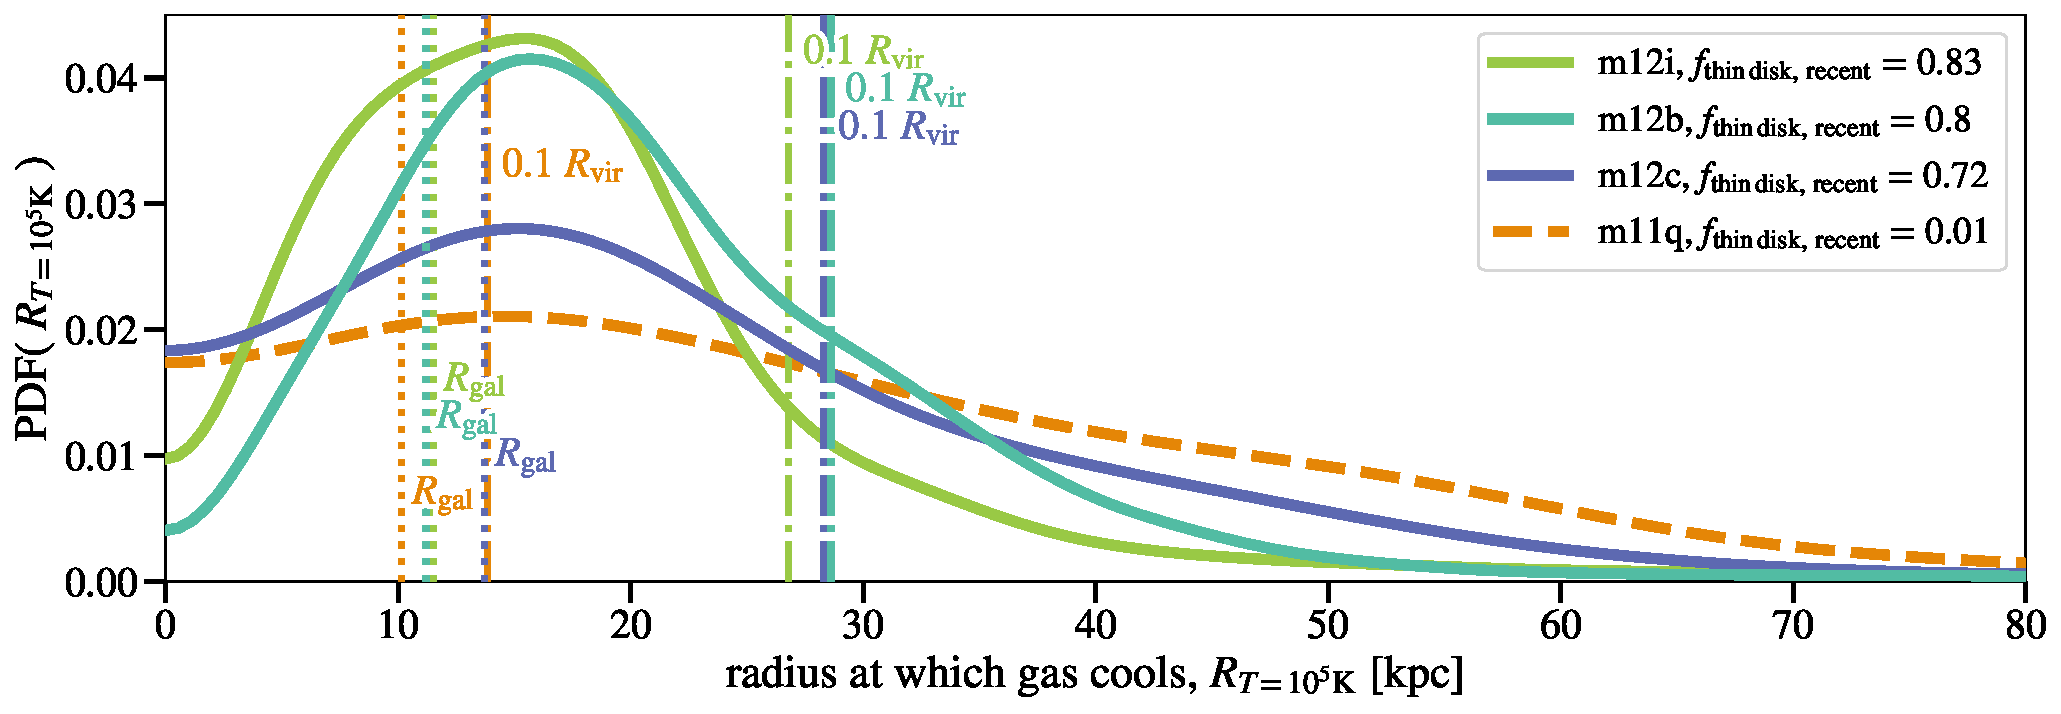
\includegraphics[width=\textwidth]{figures/R1e5K.pdf}
%     \caption{
%     Radius $\Rcon$ at which gas particles cools below $T=10^5$ K for the last time prior to accreting.
%     Gas cooling onto MW-mass disk galaxies peaks at the galaxy-halo interface, i.e. outside $R_{\rm gal}$ and within 0.1 $R_{\rm vir}$.
%     The absence of accretion that cools outside the inner CGM ($\Rcon \gtrsim 0.2 R_{\rm vir}$) is evidence that gas accretion onto MW-mass FIRE galaxies is not the result of hydrodynamic instabilities at large radii.
%     In the lower-mass halo gas cools at a broader variety of radii relative to $R_{\rm vir}$, with the $\Rcon$ distribution extending beyond $0.4 R_{\rm vir}$.
%     \textbf{Check what bin I place the particles with $R > 80$ kpc in.}
%     }
%     \label{f: R1e5K}
% \end{figure*}


\subsection{Cooling of accreted gas is concurrent with circularization}
\label{s: characteristics -- aligns}

% ORIENTS AS IT COOLS
\begin{figure*}
    \centering
    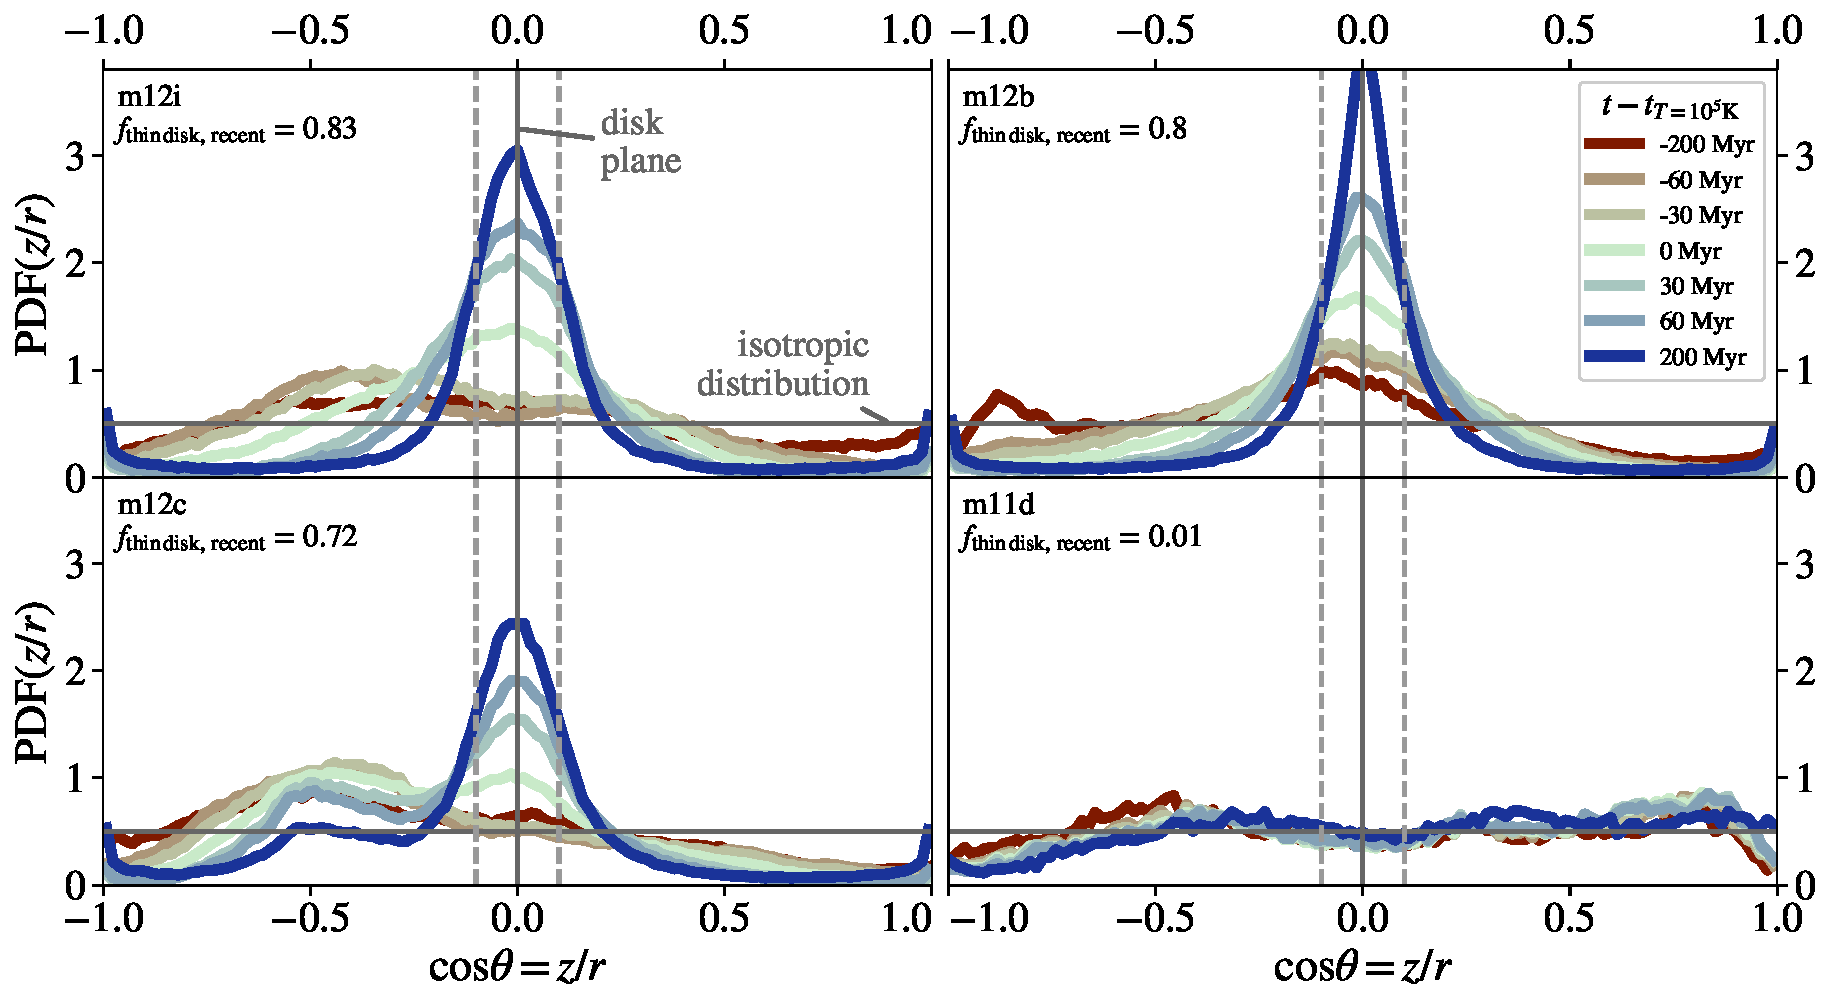
\includegraphics[width=\textwidth]{figures/theta_vs_t.pdf}
    \caption{
    Angular distribution of accreting gas, as a function of time relative to the last cooling time. In thin disk galaxies (top and bottom-left panels) the angular distribution of accreting gas evolves significantly at the time of cooling, from a quasi-spherical distribution prior to cooling to a disk-like configuration after cooling. 
    In contrast, in the irregular galaxy (bottom-right) accreting gas is roughly spherical both prior to and after cooling.
    % \textbf{Check time bin size.}
    }
    \label{f: theta vs t}
\end{figure*}

% Figure description/introduction
Panel (C) in Fig.~\ref{f: before and after A} shows that at the time of cooling the gas collapses to a median height of $\approx 2$ kpc, indicating a disk geometry with height to radius ratio of $\vert z\vert/R_{\rm gal}\approx0.2$, consistent with the transition to rotation support indicated by panel (D). This correspondence between a transition to disk geometry and cooling is further explored in Figure~\ref{f: theta vs t}, which plots the geometry of accreting gas at different times relative to $\tcon$, for the four galaxies shown in Fig.~\ref{f: stars}. 
Times prior to cooling are colored in red, while times after cooling are plotted in blue. All particles with $t-\tcon$ within $\pm$30 Myr of the value noted in the legend are included in the distribution. 
The curves show the PDF of $\cos \theta = z/r$, i.e.\ $\theta$ is the angle between the gas element position and the total angular momentum vector of stars in the galaxy.
A spherical distribution of accreted gas would have a flat PDF with a value of 0.5, while 
the PDF of an infinitely thin disk would be a $\delta$-function centered at $z/r = 0$.
The figure shows that gas accreting onto the three thin disk galaxies transitions from being distributed quasi-spherically at $t = \tcon-200$ Myr to being distributed in the galaxy plane at $t = \tcon+200$ Myr.
This indicates that cooling and circularization of the accreted gas occurs simultaneously in these galaxies, consistent with the conclusion from Figs.~\ref{f: overview} and \ref{f: before and after A}. In contrast, in the irregular galaxy shown in the bottom-right there is no association between cooling and circularization. Rather, the geometry of accreting gas is quasi-spherical both before and after cooling. 

% \subsection{The prevalence of rotating cooling flows}
% \label{s: prevalence}

% PREVALENCE OF QUIET ACCRETION
\begin{figure*}
    \centering
    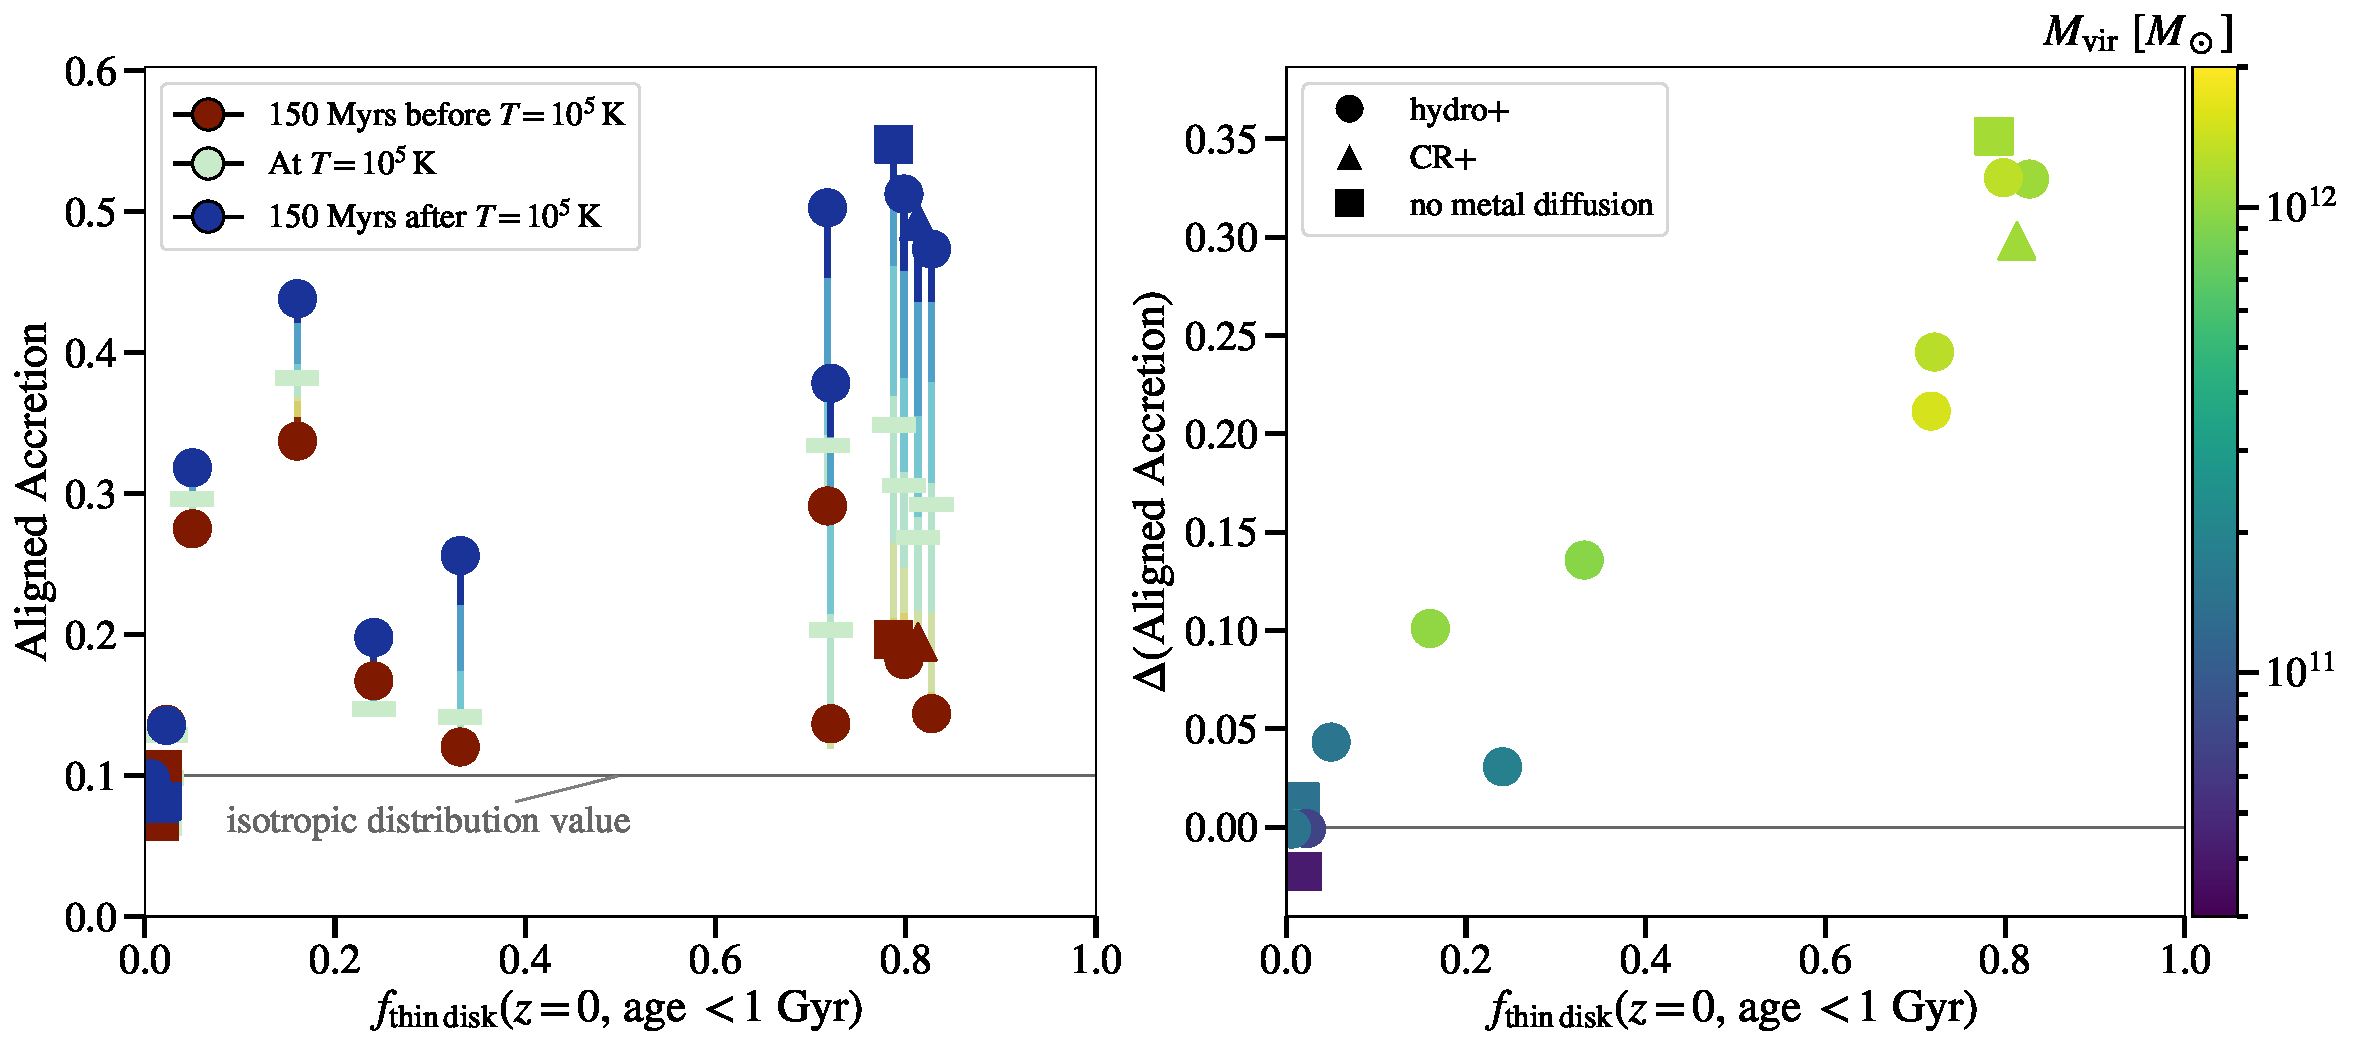
\includegraphics[width=\textwidth]{figures/prevalence/aligned_fraction.pdf}
    \caption{
    \textbf{Left:}
    Mass fraction of accreting gas aligned with the disk ($\vert z/R < 0.1 \vert$, see Fig.~\ref{f: theta vs t}) before and after cooling, for our sample of \Nsample~FIRE halos. The horizontal axis plots the fraction of young stars in the central galaxy that are in a thin disk.
    % Prior to cooling $\lesssim 30\%$ of accreting gas is strongly aligned with the galaxy plane across our simulation sample,
    % while after cooling that fraction increases to $\gtrsim 50\%$ for most galaxies forming thin disks.
    \textbf{Right:}
    Change in aligned mass fraction during the $\pm200$ Myr around cooling time shown in the left panel. A large $\Delta f_{\rm aligned}$ indicates that circularization is concurrent with cooling. Color indicates virial mass. The value of $\Delta f_{\rm aligned}$ is strongly correlated with the fraction of young stars in a thin disk. 
    % \textbf{Circle and talk about the outlier?}
    % \textbf{Highlight the empty corner?}
    }
    \label{f: prevalence}
\end{figure*}


% Figure description
% We now extend our analysis to our full simulation sample, in order to understand in which galaxies accreting gas concurrently cools and circularizes. 
Figure~\ref{f: prevalence} extends the analysis in Fig.~\ref{f: theta vs t} to the full sample. We parametrize the extent to which circularization and cooling are concurrent via a parameter $f_{\rm aligned}$, which corresponds to the fraction of accreting gas mass aligned with the disk plane ($\vert z/R \vert < 0.1$, marked by dashed vertical lines in Fig.~\ref{f: theta vs t}). This range of angles contains $\approx 60\%$ of young stars in thin disk galaxies.
The left panel of Fig.~\ref{f: prevalence} shows the evolution of $f_{\rm aligned}$ from 200 Myr before $\tcon$ (red) to 200 Myr after $\tcon$ (blue), while the right panel shows the difference in $f_{\rm aligned}$ between these two epochs. The horizontal axes plot the fraction of young stars in a thin disk $f_{\rm thin\,disk,\,recent}$. 
For most halos the accreting gas is largely unaligned prior to cooling, with aligned mass fractions $f_{\rm aligned}\sim 0.1 - 0.2$ comparable to $f_{\rm aligned} = 0.1$ expected for an isotropic distribution.
Upon cooling, the alignment of accreting gas sharply increases in halos with $f_{\rm thin\,disk,\,recent} > 0.5$ --- in most cases $\gtrsim 50\%$ of mass collapses to $\vert z/R \vert < 0.1$ during this time. In contrast, in halos with $f_{\rm thin\,disk,\,recent} \approx 0$ there is practically no change in $f_{\rm aligned}$ upon cooling. Intermediate cases with $f_{\rm thin\,disk,\,recent} \approx 0.2-0.4$ typically show a modest increase in $f_{\rm aligned}$ and are further discussed in appendix~\ref{s: appendix-individual}. The right panel of Fig.~\ref{f: prevalence} demonstrates the strong correlation between the change in $f_{\rm aligned}$ when the gas cools and the fraction of young stars in a thin disk. 
% To track the trend we draw a simple line between $(f_{\rm thin\,disk,\,recent}, \Delta f_{\rm aligned}) = (0,0)$ and the average $(f_{\rm thin\,disk,\,recent}, \Delta f_{\rm aligned})$ for galaxies with $f_{\rm thin\,disk,\,recent} > 0.5$.
% Halos with $f_{\rm thin\,disk,\,recent} > 0.5$ have $\Delta f_{\rm aligned} > 0.2$ and halos with $f_{\rm thin\,disk,\,recent} < 0.5$ have $\Delta f_{\rm aligned} < 0.2$, including four halos with $0.1 < f_{\rm thin\,disk,\,recent} < 0.5$.
Fig.~\ref{f: prevalence} thus demonstrates on our entire FIRE sample that circularization is concurrent with cooling in accretion onto thin-disk galaxies, while no such association exists for accretion onto irregular / thick disk galaxies.




% \subsection{How rotating cooling flows collapse into disks}
% \label{s: mechanics}

% COHERENCE EVOLUTION
\begin{figure*}
    \centering
    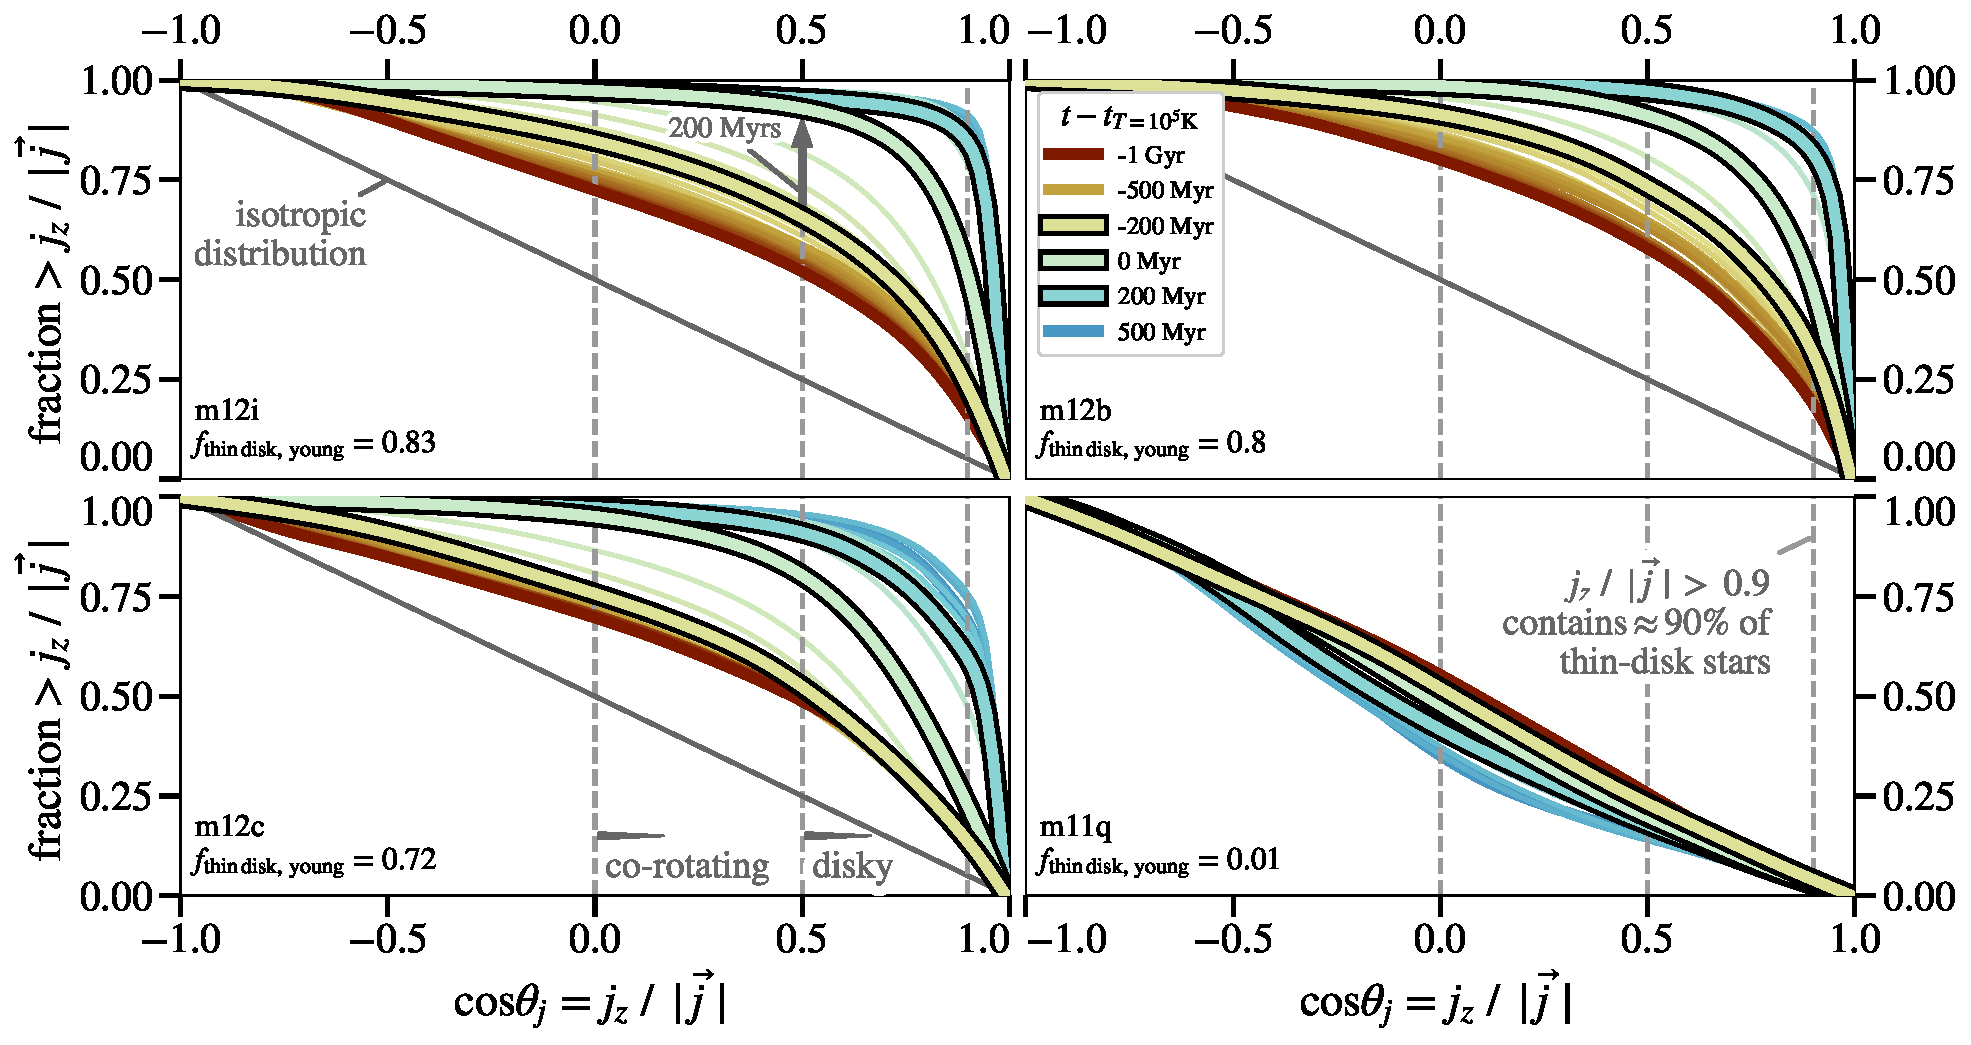
\includegraphics[width=\textwidth]{figures/jzjmag_vs_t.pdf}
    \caption{
    Angular momentum distribution of accreting gas, as a function of time relative to the last cooling time. Curves show the fraction of mass above a given $j_z / \vert \vec j \vert$. 
    In the thin-disk galaxies (top and bottom-left panels) the angular momentum distribution becomes more coherent and aligned with the central galaxy with time, mainly during the $\pm200$ Myr around the time of cooling. In the irregular galaxy (bottom right) the angular momentum distribution is quasi-spherical both before and after cooling. 
    % \textbf{How far back in time do we need to go to get to isotropic?}
    % \textbf{How does this compare to the DM distribution, e.g. B01?}
    }
    \label{f: coherence}
\end{figure*}

% MECHANICS OF QUIET ACCRETION
\begin{figure*}
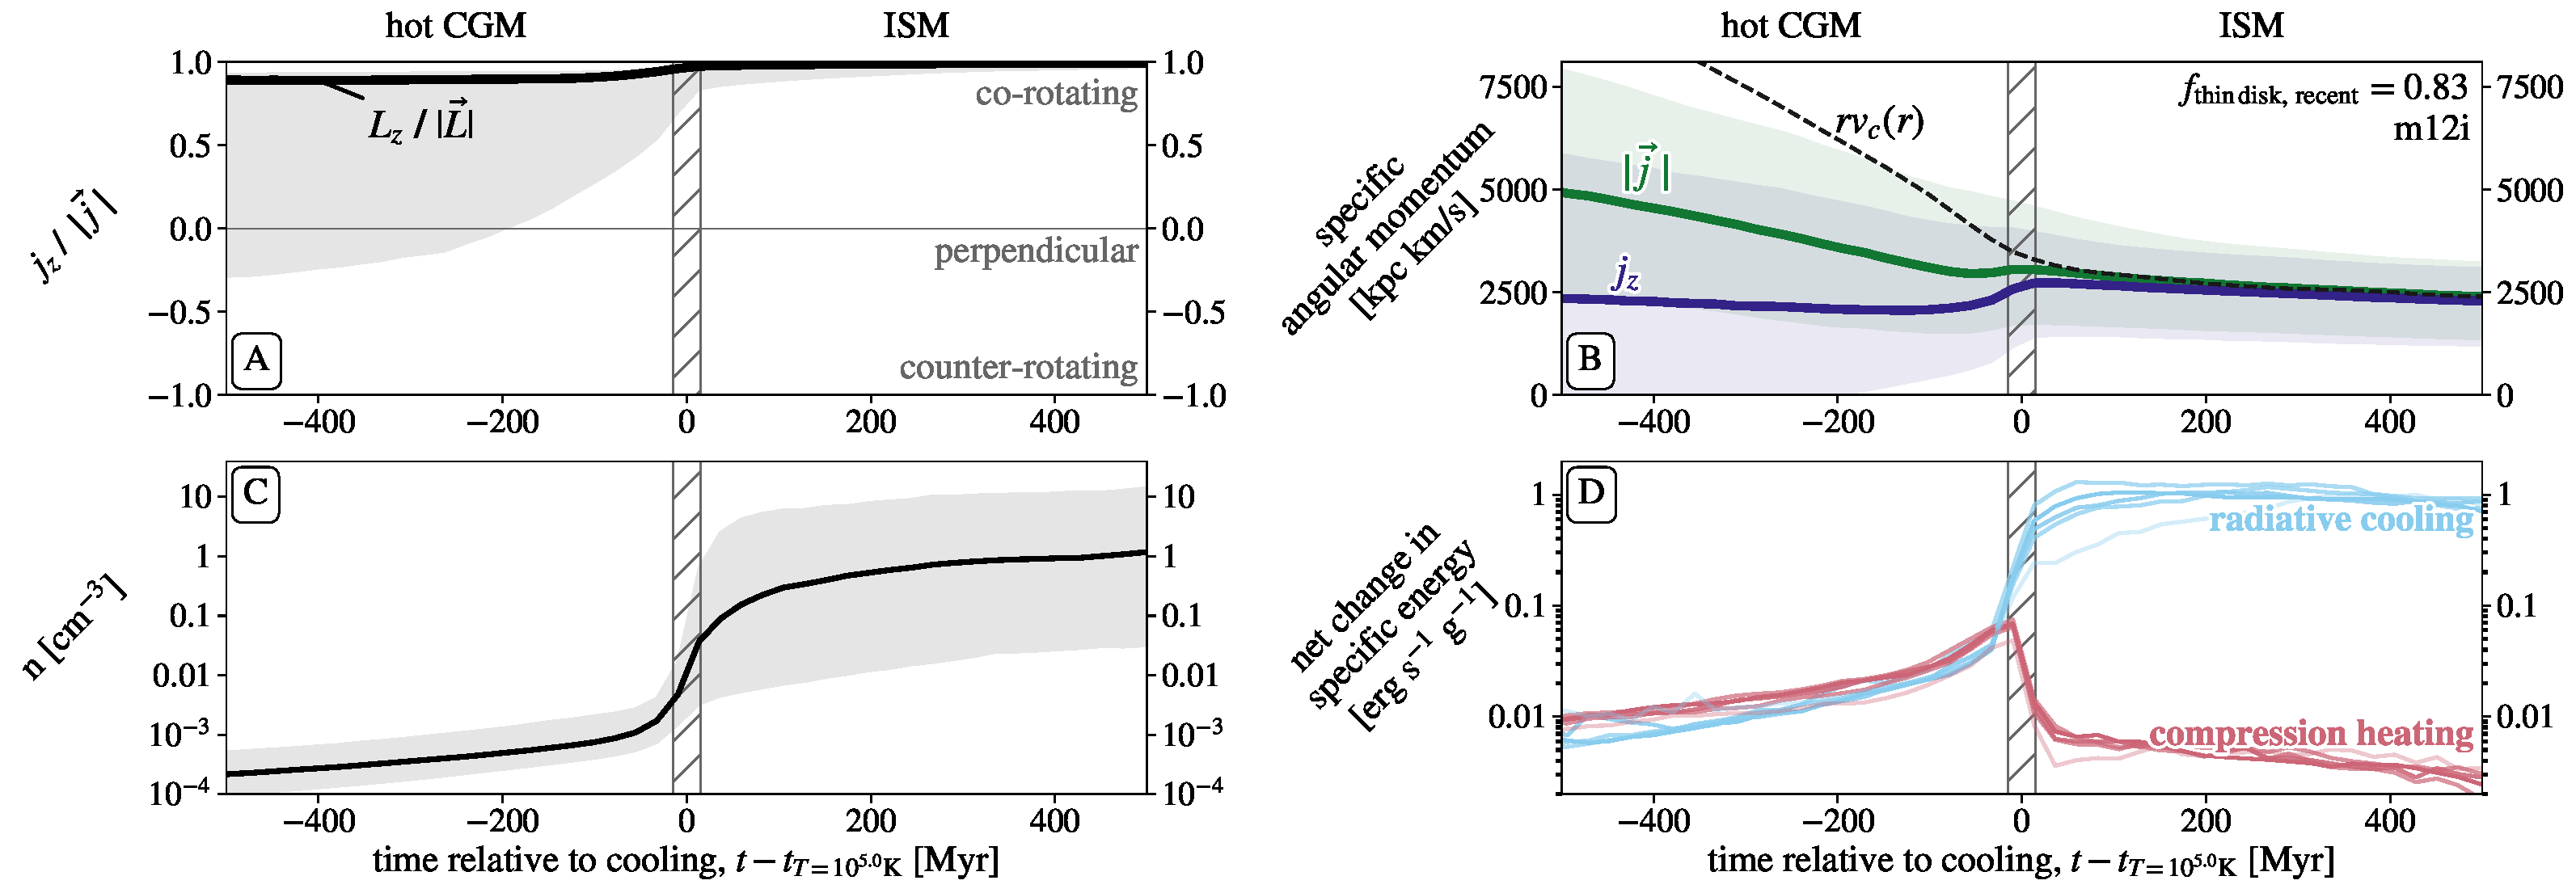
\includegraphics[width=\textwidth]{figures/before_and_after/before_and_after_m12i_md.pdf}
\caption{
Angular momentum and energetics of gas accreting onto a $z\sim0$ thin disk galaxy in FIRE, versus time relative to the final cooling time ($t - \tcon$).
In each panel solid lines and shaded regions mark the medians and 16th to 84th percentile ranges of all particles accreted within 1 Gyr prior to $z=0$.
\textbf{A:}
The ratio of $j_z / \mid \vec j \mid$. The dashed line shows this ratio for the total angular momentum of all accreted particles.
The shaded region shrinks as gas flows inward, indicating the flow becomes more coherent and that angular momentum unaligned with the total angular momentum is cancelled out, as suggested by Fig.~\ref{f: coherence}. 
\textbf{B:}
The magnitude of the specific angular momentum of particles ($\mid\vec{j}\mid$, green) and the component of angular momentum aligned with the galaxy disk ($j_z$; purple).
The dashed line shows the angular momentum necessary for rotational support.
Prior to cooling $j_z$ is conserved in the inflow. Cooling occurs when angular momentum support becomes significant, as expected in subsonic cooling flows \citep{Cowie1980, Stern2020a}.
\textbf{C:}
Baryon number density.
Prior to cooling the gas density increases due to the inflow. As the gas cools the density sharply increases, due to the stalling of the inflow at the galaxy scale and the collapse into a disk geometry. 
\textbf{D:}
Energy loss from radiative cooling (blue) and heating from $PdV$ work on the gas particles (red).
Prior to cooling compression heating offsets radiative cooling yielding the flat temperature profile seen in Fig.~\ref{f: before and after A}, as expected in a cooling flow. 
}
\label{f: before and after B}
\end{figure*}




\subsection{Angular momentum coherence in accreted gas}
\label{s: mechanics -- coherence}

% Figure coherence description
Figure~\ref{f: coherence} shows the cumulative distribution function of $j_z / \vert \vec j \vert$ in the accreted gas, weighted by mass, for the four simulations shown in Figure~\ref{f: theta vs t}. This ratio provides an estimate for the alignment of  angular momentum in the accreted gas with the rotation axis of the stars. For reference, co-rotating gas has $j_z / \vert \vec j \vert = 1$, while perpendicular and counter-rotating gas have $j_z / \vert \vec j \vert = 0$ and $-1$, respectively. An isotropic distribution of angular momentum would appear as a diagonal line in this plot. 
% The displayed distributions center on 6 times evenly spaced over $- 1\, {\rm Gyr} < t_{\rm bin} - \tcon < 0.5\, {\rm Gyr}$.
Each curve corresponds to a different $t - \tcon$ as noted in the legend. 
% The rightmost dashed grey $j_z / \vert \vec j \vert = 0.9$ line indicates the range of values containing $\approx 90\%$ of thin disk stars.
Outlined in black are the CDFs for the three times plotted in Fig.~\ref{f: prevalence}: $t - \tcon =$ -200, 0, 200 Myr.
% As in Figure~\ref{f: theta vs t}, the z-axis is aligned with the total angular momentum of the stellar component within $R_{\rm gal}$.

% Overall evolution
In gas accreting onto thin disk galaxies (top and bottom-left panels of Fig.~\ref{f: coherence})  the angular momentum distribution becomes increasingly coherent with time relative to $\tcon$. At $t-\tcon=-1$ Gyr the angular momentum distribution is relatively incoherent, with only $\approx50\%$ of accreting gas having $j_z/\vert \vec j \vert > 0.5$. In contrast at $t-\tcon=+500$ Myr the distribution is highly coherent, with $j_z/\vert \vec j \vert > 0.9$ for $\gtrsim 90\%$ of accretion.
The majority of the evolution in coherence occurs over $\lesssim 400$ Myr centered on $\tcon$, as seen by the differences between the outlined CDFs. This increase in coherence allows the accreting gas to collapse into a thin disk as shown in Figs.~\ref{f: theta vs t}--\ref{f: prevalence}. Furthermore, this result shows that accreting gas is almost entirely co-rotating with the galaxy prior to cooling, i.e., while the accretion is still part of the galactic `hot corona'.

% Fig.~\ref{f: coherence} further demonstrates that most of the transition to coherence happens just before circularization, rather than at an earlier period. 
% Before $t = \tcon - 200$ Myr and after $t = \tcon + 200$ Myr the distributions exhibit only minor evolution.

In stark contrast with thin disk galaxies, the irregular galaxy \texttt{m11q} shown in the bottom-right panel of Fig.~\ref{f: coherence} experiences only a very mild evolution in angular momentum coherence --- angular momentum remains largely isotropic both before and after cooling.

% Before
% For thin-disk galaxies the increase in co-rotating ($j_z/\vert \vec j \vert > 0$) gas fraction or disky ($j_z/\vert \vec j \vert > 0.5$) gas fraction is largest over the 200 Myr prior to cooling.
% This increase in coherence allows the gas to collapse quickly into a disk after cooling and prior to forming stars.

% After
% The fraction of accretion with momentum characteristic of a thin-disk ($j_z / \vert \vec j \vert > 0.9$) increases only mildly over the 200 Myrs prior to $\tcon$.
% Instead, the thin-disk gas fraction increases significantly after cooling, increasing from $\approx 25-50\%$ to $\approx 60-90\%$ over 200 Myrs after $\tcon$.
% This is consistent with gas collapsing into a disk immediately as it cools, and then becoming significantly more coherent immediately afterwards.
% Figure~\ref{f: theta vs t} and the left panel of Figure~\ref{f: prevalence} are consistent with this picture---most of the flattening into a \textit{thin} disk occurs \textit{immediately after} cooling.


% Coherence
% As the gas gains support it also becomes more coherent.
The evolution of angular momentum in accretion onto thin disks is further explored in Figure~\ref{f: before and after B}, for the \texttt{m12i} simulation. Panel (A) shows the median and 16th-84th percentiles in $j_z/\vert\vec j\vert$ as a function of $t-\tcon$. The dashed line plots this ratio for the total angular momentum vector of all particles at a given $t-\tcon$. 
Consistent with Fig.~\ref{f: coherence}, at $t-\tcon=-500$ Myr the ratio $j_z/\vert\vec j\vert$ spans a large range of $\approx -0.3 - 0.9$, while by $\tcon$ nearly all the accreting gas has $j_z\approx\vert\vec j\vert$, indicating all hot accreting gas particles are co-rotating. On the other hand, the ratio $j_z/\vert\vec j\vert$ of the total angular momentum vector is nearly constant with time prior to accretion. 
These trends indicate that components unaligned with the net angular momentum are canceling out due to interaction in the hot halo, as found also by other cosmological simulations ~\citep[e.g.][]{DeFelippis2017}.

% Support
Figure~\ref{f: before and after B} panel (B) shows the magnitude of the specific angular momentum ($\vert \vec j \vert$; green) and the z-component of the specific angular momentum ($j_z$; purple).
The median value $\vert \vec j \vert$ decreases prior to cooling, from $\approx 5000$ kpc km s$^{-1}$ to $\approx 3000\,{\rm kpc\,km\,s}^{-1}$, in contrast with  $j_z$ which remains constant. The nearly constant $j_{\rm z}$ indicates the inflow conserves angular momentum in this direction, and is not subject to significant torques. 
The value of $j_z\approx 2500$ kpc km s$^{-1}$ is comparable to the average specific angular momentum of $j_{\rm DM} \simeq \sqrt{2}\lambda \Rvir \vvir$ expected in dark matter halos due to tidal torques \citep[e.g.][]{Bullock2001}. Using a typical dimensionless spin parameter $\lambda \simeq 0.035$, and the virial radius $\Rvir=270$ kpc and virial velocity $\vvir=130$ km s$^{-1}$ of this halo, we get $j_{\rm DM}\approx1750$ kpc km s$^{-1}$, i.e.~the expected average value of the dark matter is within $30\%$ of the net angular momentum of accreting hot gas shown in Fig.~\ref{f: before and after B}. 

The dashed line in panel (B) of Fig.~\ref{f: before and after B} plots the specific angular momentum necessary for gas to be fully supported by angular momentum at a given radius, i.e. $v_c(r)r$, where we use the median $r$ at the relevant $t-\tcon$ for this calculation. 
The values of $j_z$ and $v_c(r)r$ converge shortly after $t=\tcon$, indicating that cooling and a transition to rotational support occur almost simultaneously, as indicated also by Fig.~\ref{f: before and after A}. This result is consistent with 1D steady-state  cooling flow solutions which include angular momentum, which demonstrate that the hot inflow cools to $\sim10^4$ K at the radius where $j_z=v_c(r)r$, as long as the flow remains subsonic down to this radius \citep{Cowie1980, Stern2020a}.

% Note that accreting gas with angular momentum significantly misaligned with the galaxy may still become supported at an inner radius, and analysis of cosmological simulations suggests that misaligned CGMs can produce warped, misaligned, or counter-rotating disks~\citep[e.g.][]{Roskar2010, Starkenburg2019}.

% The angular momentum increase
There is small-but-noticeable increase in $j_z$ at $t \approx \tcon$.
This increase is not the focus of our analysis, but we note that it may be a result of a difference in orientation and/or amplitude between the angular momentum of the galaxy and the angular momentum of the accreting gas~\citep[e.g.][]{Danovich2012, DeFelippis2017}, which forces the accreting gas to co-rotate with the galaxy.
The explicit mechanism to increase $j_z$ may be exchange of angular momentum via gravitational torques~\citep[e.g.][]{Danovich2015} or via collisional interactions.
Any angular momentum gained is expected to be lost by other particles, driving inflow of existing gas particles in the galaxy or galaxy-halo interface~\citep[e.g.][]{Mayor1981, Pezzulli2017}.
We note that the median increase in $j_z$ upon accretion and cooling shown in Fig.~\ref{f: before and after B} is quantitatively consistent with the observed $30\%$ difference between the rotation velocity of the the Milky Way disk and its hot CGM \citep{Hodges-Kluck2016}.

\subsection{Energetics of accreting gas}
\label{s: mechanics -- energy balance}

% Density
Figure~\ref{f: before and after B} panel (C) shows the distribution of the accreting gas baryon number density  versus time relative to cooling. Prior to cooling the gas density increases steadily due to the inflow, reaching $\approx10^{-3}$ cm$^{-3}$ just before cooling at $t\lesssim\tcon$. This density is comparable to observational estimates of the hot gas density just outside the Milky Way disk (e.g.,~\cite{LiBregman2017}). At $t\approx\tcon$, the gas density sharply increases, reaching $0.1$ cm$^{-3}$ within $\approx50$ Myr, due to the deceleration induced by the stalling of the inflow upon accretion (Fig.~\ref{f: before and after A}), and due to the collapse from a quasi-spherical geometry into a disk geometry. 
% A pileup occurs at $t\approx \tcon$, 
% While the gas density increases significantly, the gas is still significantly below any threshold for star formation:
% a minimal threshold for star formation of $n = 100$ cm$^{-3}$ is designated by a horizontal line, which is still $10\times$ less than the density threshold used by the FIRE simulations.
% This suggests that simulations with an under-restrictive star formation density criterion may struggle to form thin disks, as the gas is still becoming coherent as the density increases.

% Energy balance description
In Figure~\ref{f: before and after B} panel (D) we assess the energetics of the gas to determine why it cools.
We study the energetics through two types of change in specific energy: radiative cooling (blue lines) and compression heating (red lines).
Radiative cooling per unit mass for an individual particle is calculated as $\nH^2 \Lambda / \rho$, where $\nH$ is the Hydrogen density, $\rho$ is the mass density, and $\Lambda$ is the cooling function, which we take from \cite{Wiersma2009a}.
Compressive heating per unit mass for an individual particle is calculated as $P \frac{dV}{dt} \approx \frac{ P }{ \rho^2 } \frac{ \Delta \rho }{ \Delta t }$, where $P = n k_B T$, $\Delta \rho$ is the change in density from one snapshot to the next, and $\Delta t$ is the snapshot time spacing.
Because accreting gas elements interact with other accreting gas elements thermodynamically we show the mean specific energy tracks of all gas elements binned into 100 Myr bins of $\tcon$.
To focus on the behavior of the majority of the particles we do not bin the $1\%$ of particles with the highest change in specific energy.
Some $\tcon$ bins contain much more accreting gas than others, and to reflect this we set the darkness of the lines proportional to the number of particles in the bin.

% Energy balance trend
At $t-\tcon=-500$ Myr the radiative cooling rate is $\approx0.006$ erg s$^{-1}$ g$^{-1}$, corresponding to a cooling time of $400$ Myr for the median temperature of $T=4\cdot10^5$ K at this epoch (see Fig.~\ref{f: before and after A}, panel A). At $t-\tcon =-500$ Myr the cooling time is thus comparable to the accretion time of $\approx500$ Myr. At later $t-\tcon$ but still prior to cooling, the radiative cooling rate increases due to the increase in gas density. The panel however shows that this energy loss to radiation  is nearly completely offset by compressive heating, explaining the roughly flat temperature profile at $t<\tcon$ (Fig.~\ref{f: before and after A}). 
These equalities between the cooling time and the accretion time, and between radiative cooling and compressive heating, are defining   characteristics of classic cooling flows in which angular momentum support can be neglected \citep{Mathews1978, McNamara2007, Stern2019}. 

Around $\tcon$ the cooling rate and compressive heating diverge. This can be understood by noting that the radiative cooling rate per unit mass scales as $\propto\rho\Lambda$, while the compressive heating rate scales as $\propto\epsilon d\log\rho/d t$ where $\epsilon$ is the specific thermal energy. The deceleration of the hot inflow prior to accretion onto the galaxy causes $\rho$ to increase faster than  $d\log\rho/d t$, causing the temperature to decrease. This in turn increases $\Lambda$ and decreases $\epsilon$, which further accelerates the drop in temperature. The result is gas that cools from $\approx10^6$ K to $\approx10^4$ K over the course of $\lesssim 50$ Myr.

\subsection{}

% PREVALENCE OF QUIET ACCRETION -- VS GALAXY PROPERTIES
\begin{figure*}
    \centering
    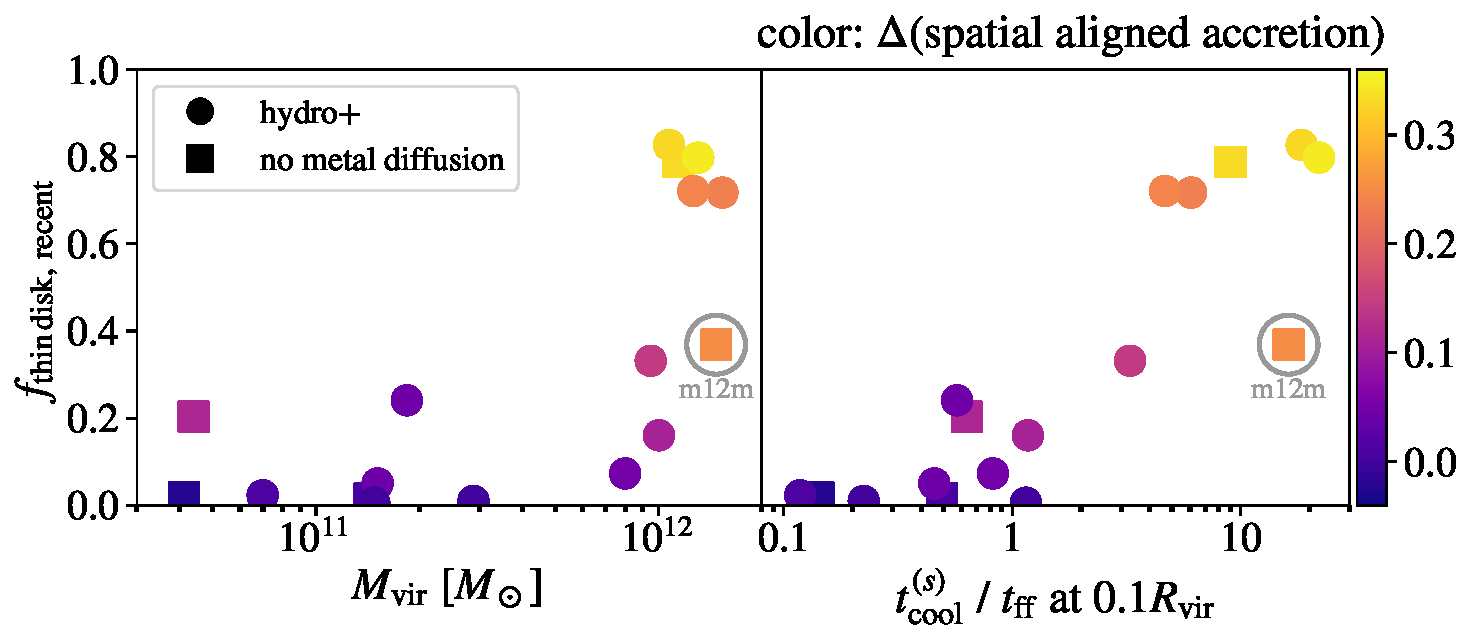
\includegraphics[width=\textwidth]{figures/prevalence/aligned_fraction_vs_galaxy_props.pdf}
    \caption{
    Fraction of young stars in a thin disk versus $M_{\rm vir}$, $M_\star$, $t_{\rm cool}^{(s)}/t_{\rm ff}$ evaluated at $0.1 R_{\rm vir}$, and Sloan-r-band-weighted thin disk fraction.
    Color indicates change in the fraction of accreted gas which is aligned with the central galaxy, during $-150\,{\rm Myr} < t-\tcon < 150\,{\rm Myr}$ (see Fig.~\ref{f: prevalence}).
    For $M_{\rm vir} < 10^{12} M_\odot$ or $M_\star < M_{\star, {\rm MW}}$, both the thin disk fraction and $\Delta f_{\rm aligned}$ are small. In more massive galaxies these quantities span a large range. A somewhat better correlation is seen between $\Delta f_{\rm aligned}$ and $t_{\rm cool}^{(s)}/t_{\rm ff}$, as expected since $t_{\rm cool}^{(s)}/t_{\rm ff}>2$ indicates that the inner CGM is virialized, a necessary condition for forming a cooling flow \citep{Stern2021}.
    The right panel shows that the thin disk fraction of young stars closely tracks the observationally-motivated luminosity-weighted thin disk fraction.
    }
    \label{f: prevalence vs galaxy properties}
\end{figure*}

% Compared to other properties
In Figure~\ref{f: prevalence vs galaxy properties} we show the relationship between the change in aligned mass fraction and virial mass, stellar mass, and the ratio of cooling time of shocked gas to freefall time at 0.1 $R_{\rm vir}$, $t_{\rm cool}^{(s)} / t_{\rm ff}$.
The cooling time is the cooling time for shocked gas, not already-dense gas.
The ratio $t_{\rm cool}^{(s)} / t_{\rm ff}$ tracks the virialization of the inner CGM (with the notable exception of \texttt{m12m}) and the onset of hot accretion~\citep{Stern2020}.
Of the three properties, only for $t_{\rm cool}^{(s)} / t_{\rm ff}$ does each $t_{\rm cool}^{(s)} / t_{\rm ff}$ correspond to a singular $\Delta f_{\rm aligned}$.
This is consistent with a cooling flow halo being a good predictor of how well gas aligns and circularizes as it cools.
The relationship between $\Delta f_{\rm aligned}$ and $M_{\rm vir}$ or $M_{\rm star}$ indicates that the change in aligned mass fraction is not solely driven by the galaxy or halo mass:
halos below $M_{\rm MW}$ all have approximately no evolution in aligned mass, and MW-mass galaxies have a wide range of $\Delta f_{\rm aligned}$.

% Compared to observable-ish thin disk fraction.
Figure~\ref{f: prevalence vs galaxy properties} also shows the relationship between $f_{\rm thin\,disk,\,recent}(z=0,$ age $<1$ Gyr) and the Sloan r band luminosity-weighted thin disk fraction, $f_{\rm thin\,disk,\,recent}(z=0,$ Sloan r band).
The luminosity-weighted $f_{\rm thin\,disk,\,recent}$ highlights the extent to which the thin disk is observationally visible, and is closely related to the young thin disk fraction.


\section{Discussion}

In this paper we analyze the properties of gas accreting onto $z\sim0$ galaxies simulated in FIRE, focusing on Milky-Way mass galaxies in which new stars form in a thin disk. 
We have arrived at two main results: 
(1) thin disk galaxies in FIRE accrete via `rotating cooling flows', a hot accretion mode in which the quasi-spherical hot CGM inflows towards the galaxy, remaining hot down to the radius where its angular momentum is sufficient to provide rotation support. At this radius, which is just outside the galaxy radius $\approx4 R_{1/2}$, the hot inflow both decelerates and becomes coherently rotating, and then simultaneously cools and collapses into a rotating cool disk. Our results thus extend classic cooling flow theory by demonstrating their applicability in realistic cosmological simulations, and by exploring the mechanics of cooling flows with angular momentum, a subject which has not yet been studied extensively \citep[c.f.][]{Cowie1980,Stern2020a}; (2) We find a strong correlation between the existence of this accretion mode and the fraction of stars formed in a thin disk, potentially suggesting a causal connection. In this section we ...

\subsection{Why do hot inflows decelerate and become coherent prior to accretion?}

The hot inflows 


Figs.~\ref{f: coherence} and 

%1. extend cooling flow theory
    %addition of AM, only briefly previously explored: new effects are circularization concurrent with cooling, angular momentum coherence
    %comparison with other models and feedback, e.g. Fraternali+ (4.2) and thermal-balance models
%2. relate cooling flows to thin disk galaxies
    %angular momentum coherence required to form thin disks (4.1.1 , 4.2.1, 4.2.3)
    %subsonic flows require to form thin disk
    %ICV likely insufficient to form disks since ICV at high z forms thick disks
    %over-predictions of SFR in FIRE (4.3) , add ref to Peebles
%3 comparison to observations

\label{s: discussion}

\subsection{Rotating cooling flows and disk formation}
\label{s: disk formation}

In \S\ref{s: characteristics} we showed rotating cooling flows collapse directly into a disk at the galaxy halo interface, in \S\ref{s: prevalence} we showed there is a strong correlation between rotating cooling flows and thin disk formation, and in \S\ref{s: mechanics} we assessed the mechanics responsible for this behavior.
We now assess several other aspects of the connection between rotating cooling flows and disk formation.

\subsubsection{Gaseous disks prior to star formation}
\label{s: disk formation -- condition}

% Star-forming gas constraints
In our simulations, thin disks at $z=0$ are composed of stars that form in a thin disk, and remain in a thin disk thereafter~\citep{Yu2021}.
This is in contrast to spheroidal and thick disk components, which may be partially composed of stars that gravitationally interacted with mergers, spiral arms, and giant molecular clouds.
If thin disks are composed of undisturbed stars then there is a  constraint on the star-forming gas that fuels them:
for a given sample of stars, the fraction of stars in a thin disk provides a lower limit on the fraction of star-forming gas in a thin disk at the time of formation, $f_{\rm thin\,disk,\,SF\,gas} \ge f_{\rm thin\,disk,\,stars}$.
For most of the thin disk galaxies in our sample this suggests $f_{\rm thin\,disk,\,SF\,gas} \gtrsim 0.8$ for star-formation within the last Gyr prior to $z=0$.

% Time-scale argument
This constraint on $f_{\rm thin\,disk,\,SF\,gas}$ subsequently constrains which accretion modes fuel thin disk formation.
Given sufficient time, radiatively-cooling gas in thermal contact will eventually form a thin disk.
At first glance this suggests that it does not matter how gas enters the galaxy:
any mode of gas accretion is capable of forming a thin disk given sufficient time for the gas to equilibriate.
However, whether or not the gas eventually forms a thin disk is less important than whether or not the gas forms a thin disk \textit{prior} to becoming star forming.
Thin-disk star-forming gas must satisfy the condition $t_{\rm thin\,disk} < t_{\rm SF}$, where $t_{\rm thin\,disk}$ is the time for gas to form a thin disk after entering the ISM and $t_{\rm SF}$ is the time for gas to become star-forming after entering the ISM.
Combined with the above constraint on $f_{\rm thin\,disk,\,SF\,gas}$, gas accretion that fuels thin-disk star-formation must satisfy
\begin{equation}
    f( t_{\rm thin\,disk} < t_{\rm SF} ) \ge f_{\rm thin\,disk,\,stars}
    \label{e: timescale constraint}
\end{equation}
noting that $f_{\rm thin\,disk,\,SF\,gas} = f( t_{\rm thin\,disk} < t_{\rm SF} )$.

% Satisfaction of condition for rotating cooling flows
Equation~\ref{e: timescale constraint} constrains which accretion modes may contribute to thin-disk star-formation.
Rotating cooling flows easily satisfy this condition:
typically $t_{\rm thin\,disk} < 200$ Myr for $\gtrsim 80\%$ of the gas accretion (Figure~\ref{f: coherence}) and $t_{\rm SF} > 500$ Myr for all gas accretion (Figure~\ref{f: before and after}; Panel F).
Therefore $f( t_{\rm thin\,disk} < t_{\rm SF} ) > 0.8$ for rotating cooling flows.

% Other modes
Exploring the extent to which other modes satisfy Equation~\ref{e: timescale constraint} is beyond the scope of our work.
However, we note that one of the defining features of a rotating cooling flow is that it forms a disk as it accretes onto the galaxy (as stated $t_{\rm thin\,disk} \lesssim 200$ Myr).
This is only possible because the gas exchanges angular momentum and gains coherence prior to accretion while the gas is in the halo (Figure~\ref{f: coherence}).
Not all accretion mechanisms may exchange angular momentum amongst accreting gas while the gas is in the halo.
For example supersonic cold flow accretion is not in thermal contact, and can therefore not equilibriate to a coherent rotation while in the halo.
Therefore cold flow accretion and other accretion modes that do not exchange angular momentum while in the halo \textit{must} take longer to form a thin disk in the galaxy than a rotating cooling flow does.
This makes satisfying Equation~\ref{e: timescale constraint} more challenging.

% Necessary but not sufficient
Note that Equation~\ref{e: timescale constraint} is a necessary-but-not-sufficient condition for thin disk star formation.
A merger, feedback event, or other disruption may take a thin gaseous disk and disturb it, preventing thin disk stars from forming.
Simulation \texttt{m12m} provides evidence of this:
it has comparable rotating cooling flow accretion to galaxies with $f_{\rm thin\,disk,\,recent}\sim 0.8$ (i.e. $\Delta f_{\rm aligned} \approx 0.25$), but only has $f_{\rm thin\,disk,\,recent} \approx 0.4$.

\subsubsection{$L^*$ halos mark a transition in galaxy and CGM properties}
\label{s: disk formation -- transition}

% Importance of L*
Galaxies with a mass comparable to the MW have long been of special interest, both because of their relation to our galaxy and because the mass is thought to be a critical mass at which many properties of galaxies and the CGM change change~\citep[e.g.][]{Fielding2017, Correa2017, Dekel2019a}.
$L^\star$ halos are at the peak of the $M_\star/M_{\rm h}$ vs $M_{\rm h}$ relation~\citep{Behroozi2019a}, suggesting they may be halos where galactic feedback is weakest.
In regards to disk formation, $M_{\rm h} \sim 10^{12} M_\odot$ halos have the highest thin disk presence~\citep[e.g.][]{Kranz2003, Kassin2006, Bizyaev2021}.
% $M_{\rm h} \lesssim 10^{11} M_\odot$ are more often irregular~(\textbf{citation n}) and $M_{\rm h} \gtrsim 10^{13} M_\odot$ halos are more often elliptical~(\textbf{CITATION NEEDED}).

% % Shea's work
% \cite{Garrison-Kimmel2018} studied the origin of MW-mass disk galaxies in the FIRE simulations, and found disk morphology can correlate well with gas accretion history, as parameterized by the spin parameter of the gas at the time half the stars have formed.
% On the other hand, dark matter accretion history correlates poorly with disk morphology, as parameterized by the time at which half the dark matter mass is assembled and also parameterized by the predicted radius of the galaxy assuming angular momentum is inherited from the dark matter.
% Our work suggests that the disk fraction is constrained by the accretion mode of gas, consistent with gas accretion history being more important than dark matter accretion history.

% FIRE-centric recent work
In the FIRE simulations properties that change at $M_{\rm h}\sim10^{12} M_\odot$ include a transition from a supersonic and free-falling inner CGM to a subsonic and virialized inner CGM;
a transition from bursty to steady star formation;
a transition from a dynamic and morphologically-disturbed ISM to a rotationally-supported ISM;
and a transition from spheroidal or thick disk to thin disk stellar morphology~(\citealt{El-Badry2018a, Stern2020, Yu2021}, Gurvich et al., in prep).
Rotating cooling flows become the main mode of accretion at the mass the halo virializes~(Figure~\ref{f: prevalence vs galaxy properties}).
If rotating-cooling-flow accretion is a condition for disk formation then this explains the correlation between the presence of a virialized halo and thin disk formation.
This is independent of the behavior of the galaxy, provided galactic feedback is not affecting the CGM in a way that disrupts the cooling flow.
As discussed in the previous section, rotating cooling flows are likely not a sufficient condition for thin disks, requiring further investigation of the formation of thin gaseous disks in the ISM (Gurvich et al., in prep).

\subsubsection{The presence or absence of thin disks in simulations}
\label{s: disk formation -- population}

% Thin stellar disk but no feedback
The conditions under which simulated galaxies produce disk galaxies also points to the role of rotating cooling flows in disk formation.
The first piece of evidence is the presence of galaxies with thin stellar disks in cosmological simulations absent strong galactic winds~\citep{Guedes2011, Bird2013}.
If disk galaxies are produced under similar conditions in these simulations and our simulations then we can deduce that an accretion mode that enables disk formation is likely one that occurs absent feedback affecting the CGM.
Rotating cooling flow accretion fits this condition well:
cooling flows are solutions for hot gaseous halos that are \textit{not} strongly affected by feedback~\citep{Stern2019}.
Instead the hot or cool nature of the halo is determined solely by the halo baryon content and/or the accretion rate, which increases with increasing dark matter halo mass~\citep{Stern2020a}.

% Underprediction of thin disks at low mass
The second piece of evidence is the underprediction in FIRE of a galaxy population with thin stellar disks for galaxies with $M_* = 10^6 \-- 2 \times 10^7 M_\odot$~\citep{El-Badry2018a}, where our galaxies are fed primarily by cold flows~\citep{Stern2020}.
If having a rotating cooling flow is a necessary condition for disk formation then the absence of rotating cooling flows in these halos also explains the underprediction of disky galaxies.
Inducing cooling flows in these halos would require the halo to have a lower baryon content, potentially requiring additional feedback physics.

% \subsubsection{Analogous accretion in halos with nonthermal support}
% \label{s: disk formation -- nonthermal}

% % Comparison to Trapp+2021
% \cite{Trapp2021} performed a thorough, complementary, phenomenological-focused analysis on the accretion of gas onto MW-mass galaxies and its transport through the disk.
% Their analysis focused on simulations that include cosmic ray feedback, and therefore provides a window into the differences in gas accretion modes in simulations with and without non-thermal support.
% \citeauthor{Trapp2021} find the following characteristics of accreting gas:
% gas primarily accretes as part of flared or funnel-like structures at the disk edge;
% gas becomes more coherent as it approaches the disk edge;
% after accreting gas co-rotates with the galaxy;
% gas becomes fully rotationally supported at the radius of accretion;
% gas moves inward more slowly after reaching the disk edge;
% and the disk edge is produced by a density-increasing pileup.

% % Comparison to rotating cooling flows
% All of the characteristics of accreting gas identified by \citeauthor{Trapp2021} are consistent with the characteristics of rotating cooling flow accretion.
% Further, we processed one simulation with cosmic ray feedback---\texttt{m12i\_cr}, a MW-mass halo with a thin disk.
% We confirm that \texttt{m12i\_cr} has very similar accretion to the other thin disk galaxies:
% the triangle marker in Figure~\ref{f: prevalence} is for \texttt{m12i\_cr} and Appendix~\ref{s: appendix-crs} shows Figure~\ref{f: before and after} for \texttt{m12i\_cr}.

% % Implications
% This accretion analogous to a rotating cooling flow occurs despite the fact that cosmic rays provide non-thermal support to the accreting gas and therefore cooling flow solutions are not necessarily valid --- as stated previously, cooling flow solutions are for radiatively cooling gas with no feedback terms~\citep[e.g.][]{Stern2019}.
% This similar accretion is a preliminary demonstration that the mechanisms responsible for rotating cooling flows are valid for a larger range of situations than shown in this paper.
% The mechanics discussed in~\S\ref{s: mechanics} are consistent with this finding ---
% the gas collapses into a disk because it is coherent prior to becoming rotationally supported, which is enabled by the gas exchanging angular momentum in the halo.
% Any other accretion mode that also has a voluminous, rotating, radiatively-cooling gaseous halo might be expected to also satisfy these conditions.

\subsection{Related work on disk formation}
\label{s: other disk formation}

\subsubsection{Angular momentum alignment}
\label{s: other disk formation -- alignment}

% Angular momentum alignment
In rotating cooling flows the alignment of the angular momentum is essential to providing disky accretion.
A number of previous studies have similarly noted that angular momentum alignment is crucial for disk formation.
For example, \cite{Sales2012} find in their cosmological simulations that angular momentum alignment of accreting gas is better correlated with disk formation than any dark matter halo property.
\cite{Kretschmer2020} similarly point to the alignment of angular momentum as the distinguishing factor between a cosmological zoom-in of a disk galaxy and a zoom-in of a bulge-dominated galaxy with similar mass accretion histories and halo spin parameters.
Rotating cooling flows may explain how alignment contributes to disk formation.

\subsubsection{Feedback-driven accretion}
\label{s: other disk formation -- feedback-driven}

% Coronal mixing
Hydrodynamical models suggests that accretion can be induced by cold clouds launched into the galaxy-halo interface via galactic feedback~\citep[e.g.][]{Marinacci2010, Marinacci2011, Marinacci2012, Armillotta2016a, Fraternali2017}.
These models are consistent with observations of extraplanar neutral gas rotating in the same direction as the galaxy but with some lag~\citep[e.g.][]{Fraternali2008,  Marasco2012}.
In this ``feedback-induced'' accretion hot halo gas only cools when its cooling time is lowered by mixing with cold gas ejected from the galaxy.
Feedback-induced accretion may be conducive to ongoing disk formation --- if the gas ejected from the disk preserves its angular momentum magnitude and orientation and if the hot halo is largely co-rotating with the galaxy then the induced accretion may also have a disky morphology.
On the other hand, the accretion rate from feedback-induced accretion may increase with star formation rate~\citep{Hobbs2020}, which could promote a clumpy morphology.
Understanding how rotating cooling flow accretion and feedback-induced accretion interact warrants further work.
For now we note that rotating cooling flows cool out of the halo as a result of decreased compression heating and increased pileup from density, i.e. without feedback.
In fact, in rotating cooling flow accretion the majority of cooling occurs at the outer rim of the galaxy~(Figure~\ref{f: R1e5K}), before feedback can induce cooling.
Subsequently, rotating cooling flows should provide accretion conducive to disk formation regardless of the presence of a disk galaxy.

\subsubsection{Cold flow disks}
\label{s: other disk formation -- cold flow disks}

% Cold flow disks
Previous studies have also looked at disks formed out of cold mode accretion, often focusing on extended ``cold flow disks'' orbiting the galaxy~\citep[e.g.][]{Stewart2011a}.
For example, \cite{Stewart2013} demonstrate that in cosmological simulations cold mode accretion has $\sim 70\%$ more specific angular momentum than hot mode accretion and dark matter, which may explain the presence of these disks.
\cite{Danovich2015} show that cold flow disks can be torqued to be aligned with the central galaxy, an alignment that is aided by outflows simultaneously preferentially ejecting low angular momentum gas~\citep[e.g.][]{Ubler2014}.
More recently, \cite{Dekel2019} propose that cold flow disks become permanent when the central galaxy reaches a sufficient mass such that the orientation of the galaxy is not being routinely flipped by major mergers.

% Thickness of disk
However, cold flow disks are significantly thicker than the disks we study.
In \cite{Dekel2019} the ratio of the disk radius to the half height for $T < 1.5 \times 10^4$ K gas spans $\approx 4-6.4$, while for \texttt{m12i} at $z=0$ the same ratio calculated using the same definitions is 9.6.
In our sample the unvirialized \texttt{m11h} is the closest to being a cold flow disk with a ratio of 4.5.
If angular momentum alignment prior to accretion determines the thinness of the disk, as our analysis suggests, then cold mode accretion should naturally produce thicker disks than hot mode accretion because the gas cannot interact and subsequently align to the same extent.

\subsection{Star formation rates fueled by rotating cooling flows}
\label{s: fueling}

% Overprediction of star formation
In our MW-mass halos the average SFR over $z=0-0.5$ is SFR$\approx 3-10\,M_\odot/$yr, while the observationally-based average SFR for $M_{\rm vir} \sim 10^{12} M_\odot$ halos over the same redshift range is SFR$\approx 0.7-6\,M_\odot/$yr~\citep{Behroozi2013}.
FIRE simulations also underpredict the number of red galaxies~\citep{Garrison-Kimmel2017}.
Given that in FIRE SFR is regulated by $\Mdot$ (Fig.~\ref{f: Mdot}), this potential discrepancy may be a result of an elevated CGM accretion rate relative to the real accretion rate.

The CGM accretion rate may be reduced by including additional feedback to suppress star formation, such as cosmic rays~\citep{Chan2019, Hopkins2020, Hopkins2020a, Hopkins2020b}
or AGN feedback (Wellons et al. in prep.). 
Our result that MW-mass galaxies are fed by a cooling flow suggests an alternative solution to this problem: that the CGM mass or metallicity are somewhat overpredicted in MW-mass halos in FIRE.
This follow since in a cooling flow $\Mdot\propto M_{\rm CGM}^2 \Lambda(Z)$, so if the CGM mass is overpredicted by a factor of two, then $\Mdot$ and the SFR would be overestimated by a factor of four.
Both the CGM mass and metallicity are a result of the integrated enrichment and depletion of the CGM by outflows over cosmic time, and thus are somewhat uncertain~\citep{Kelly2021}.
A lower CGM mass than suggested in FIRE would also be more consistent with several studies of X-ray emission from the MW which find $M_{\rm CGM}/f_bM_{\rm halo} \approx 0.1$~\citep[][]{Faerman2017, Li2018, Bregman2018}, where $f_b M_{\rm halo}$ is the cosmological baryon fraction multiplied by the halo mass, i.e. the maximum number of baryons the halo could contain given no feedback.
This is in contrast with $M_{\rm CGM}/f_bM_{\rm halo} \approx 0.2-0.4$ for similar-mass FIRE halos~\citep{Hafen2019}, though note that other studies deduce $M_{\rm CGM}/f_bM_{\rm halo}=0.3$ based on the same X-ray data~\citep{Faerman2019}.
A lower CGM mass in units of the halo baryon budget may also help alleviate the discrepancy wherein the $z\sim0$ thin disk fraction predicted by FIRE is lower than the observed value for galaxies with $M_{\rm vir} \lesssim 10^{11} M_\odot$~\citep{El-Badry2018, Peebles2020, Stern2020}.
This follows since a lower $M_{\rm CGM}$ implies that $t_{\rm cool}$ exceeds $t_{\rm ff}$ and the inner CGM can virialize at lower halo masses~\citep{Stern2020}, which given the relation between virialization and thin disk fraction found above would increase the thin disk fraction relative to that predicted by FIRE. 

\section{Conclusions}
\label{s: conclusions}

% Summary paragraph
In this paper we studied the characteristics, prevalence, and mechanics of accretion onto MW-mass disk galaxies at $z \sim 0$ (Figure~\ref{f: stars}).
Our analysis was centered on the history of gas found inside MW-like FIRE-2~\citep{Hopkins2018b} simulated galaxies at $z=0$, and outside one Gyr prior.
Our main takeaways are as follows.
\begin{itemize}
    \item \textbf{Characteristics (\S\ref{s: characteristics}):}
    Rotating cooling flows are a mode of cosmological accretion wherein hot CGM inflow (Figure~\ref{f: Mdot}) cools at the galaxy-halo interface (Figure~\ref{f: R1e5K}), and as it cools it collapses into a disk oriented with the galaxy (Figure~\ref{f: theta vs t}).
    A visual overview is provided in Figure~\ref{f: overview}.
    \item \textbf{Prevalence (\S\ref{s: prevalence}):}
    Rotating cooling flows are the main accretion mechanism for galaxies forming thin disks and rotating cooling flows are much weaker or absent for galaxies not forming thin disks --- 
    across a sample of \Nsample~galaxies spanning $10^9 M_\odot < M_\star < 10^{11} M_\odot$, the fraction of thin disk stars formed is strongly correlated with the fraction of gas accreted as a rotating cooling flow (Figure~\ref{f: prevalence}).
    All galaxies that form half or more of their stars in a thin disk are fueled primarily by rotating cooling flows.
    The correlation between between thin disk fraction and rotating cooling flow accretion is stronger than the correlation between thin disk fraction and stellar or halo mass (Figure~\ref{f: prevalence vs galaxy properties}).
    \item \textbf{Mechanics (\S\ref{s: mechanics}):}
    The correlation between rotating cooling flows and disk formation is enabled by angular momentum exchange amongst the hot accreting gas, which builds a coherent angular momentum distribution prior to accretion (Figure~\ref{f: coherence}).
    This allows the accreting gas to collapse quickly into a disk when it cools.
    As outlined in Figure~\ref{f: before and after}, cooling occurs when the gas becomes rotationally supported --- this both causes a pileup that increases density and therefore radiative cooling, and at the same time halts compression heating driven by inward movement.
\end{itemize}

% Discussion summary
We discussed how rotating cooling flows drive disk formation (\S\ref{s: disk formation}), including the importance of forming a thin gaseous disk prior to star formation (\S\ref{s: disk formation -- condition}), the unique role of MW-mass disks (\S\ref{s: disk formation -- transition}), and the existence of an analogous accretion mode in halos with nonthermal support (\S\ref{s: disk formation -- nonthermal}).
We compared disk formation via rotating cooling flows to feedback-induced accretion (\S\ref{s: other disk formation -- feedback-driven}) and cold flow disks (\S\ref{s: other disk formation -- cold flow disks}), other routes through which cosmological accretion may enable disk formation (\S\ref{s: other disk formation}).
Finally, we noted that decreasing the baryon mass or metallicity of FIRE-2 gaseous halos may bring some simulation properties into better alignment with observations (\S\ref{s: fueling}).

% Final paragraph
\cite{Trapp2021} find gas infall at the galaxy-halo interface of FIRE-2 $L^*$ galaxies is roughly consistent with observational constraints on mass flux~\citep[e.g.][]{Putman2012, Rohser2016} and cloud infall speed~\citep[e.g.][]{Zheng2017, Werk2019, Bish2019, Ho2020}.
Comprehensive mock observations may be necessary to provide testable predictions, and to enable identification of galaxies undergoing rotating cooling flows, potentially including our own.
The relationship between rotating cooling flows, disk formation, and a transition in galaxy and CGM properties needs to be further disentangled, with causal directions determined (Gurvich et al., in prep).
To this end, analyses that probe the parameter regime over which rotating cooling flows occur in cosmological simulations (including redshift and halo mass) would be valuable.

\section*{Acknowledgements}

\textbf{TBD.}

\textbf{Halo21 KITP workshop/ KITP primary grant number NSF PHY-1748958.
This research was supported in part by the National Science Foundation under Grant No. NSF PHY-1748958.
}


%%%%%%%%%%%%%%%%%%%%%%%%%%%%%%%%%%%%%%%%%%%%%%%%%%

%%%%%%%%%%%%%%%%%%%% REFERENCES %%%%%%%%%%%%%%%%%%

% The best way to enter references is to use BibTeX:

\bibliographystyle{mnras}
\bibliography{references,jsbref} % if your bibtex file is called example.bib

% Alternatively you could enter them by hand, like this:
% This method is tedious and prone to error if you have lots of references
%\begin{thebibliography}{99}
%\bibitem[\protect\citeauthoryear{Author}{2012}]{Author2012}
%Author A.~N., 2013, Journal of Improbable Astronomy, 1, 1
%\bibitem[\protect\citeauthoryear{Others}{2013}]{Others2013}
%Others S., 2012, Journal of Interesting Stuff, 17, 198
%\end{thebibliography}

%%%%%%%%%%%%%%%%%%%%%%%%%%%%%%%%%%%%%%%%%%%%%%%%%%

%%%%%%%%%%%%%%%%% APPENDICES %%%%%%%%%%%%%%%%%%%%%

\appendix

\section{Observed thin disk fraction}
\label{s: appendix-sloan thin disk fraction}

% PREVALENCE OF QUIET ACCRETION -- VS GALAXY PROPERTIES
\begin{figure}
    \centering
    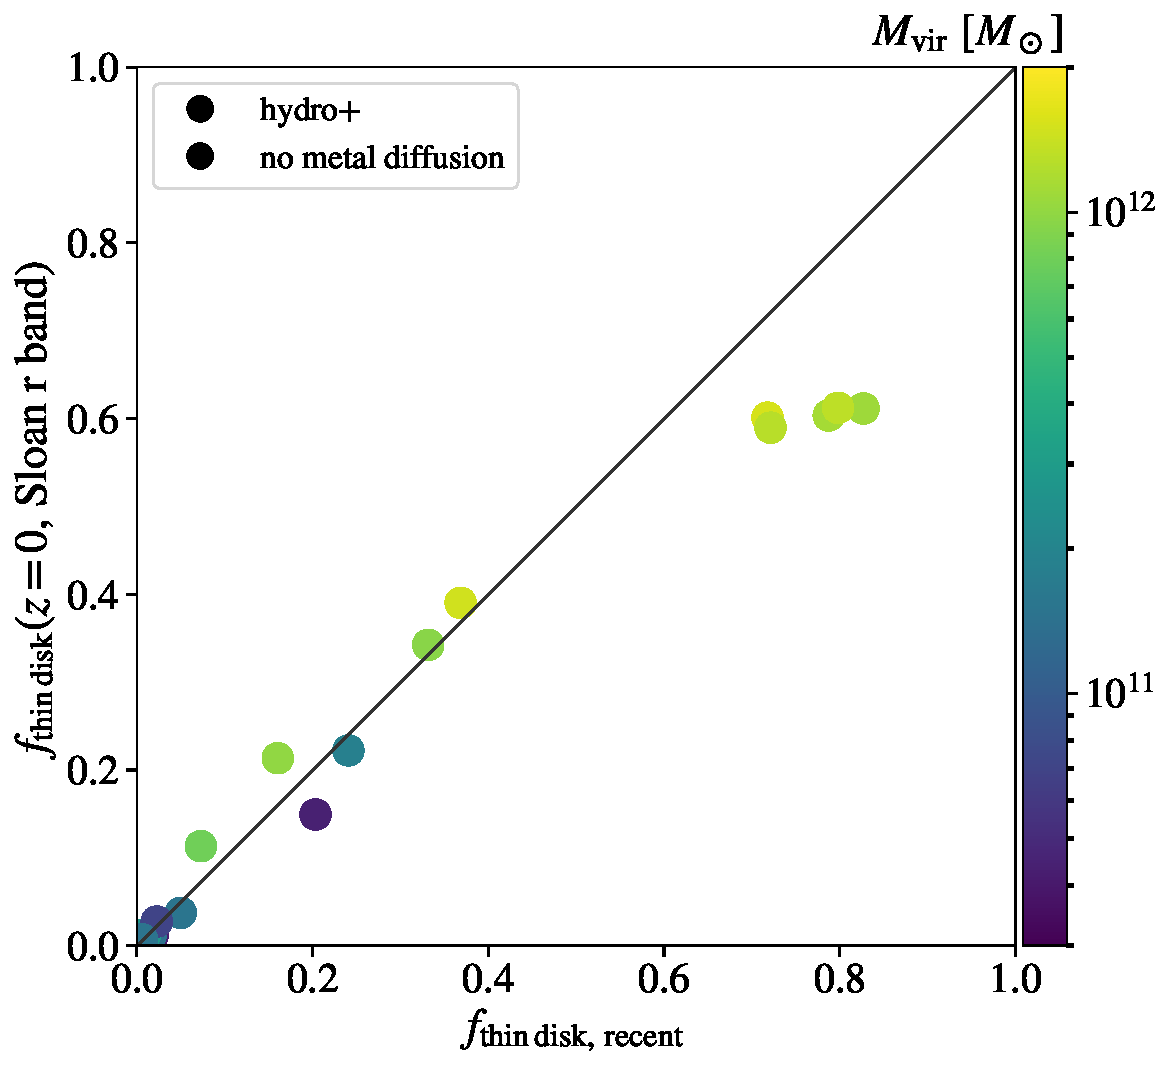
\includegraphics[width=\columnwidth]{figures/prevalence/thin_disk_v_thin_disk.pdf}
    \caption{
    Fraction of recent stars in a thin disk versus Sloan-r-band-weighted thin disk fraction, showing that the thin disk fraction of young stars closely tracks the observationally-motivated luminosity-weighted thin disk fraction.
    }
    \label{f: thin disk v thin disk}
\end{figure}

\section{Accretion onto lower-mass halos}
\label{s: appendix-lowmass}

% MECHANICS OF QUIET ACCRETION
\begin{figure*}
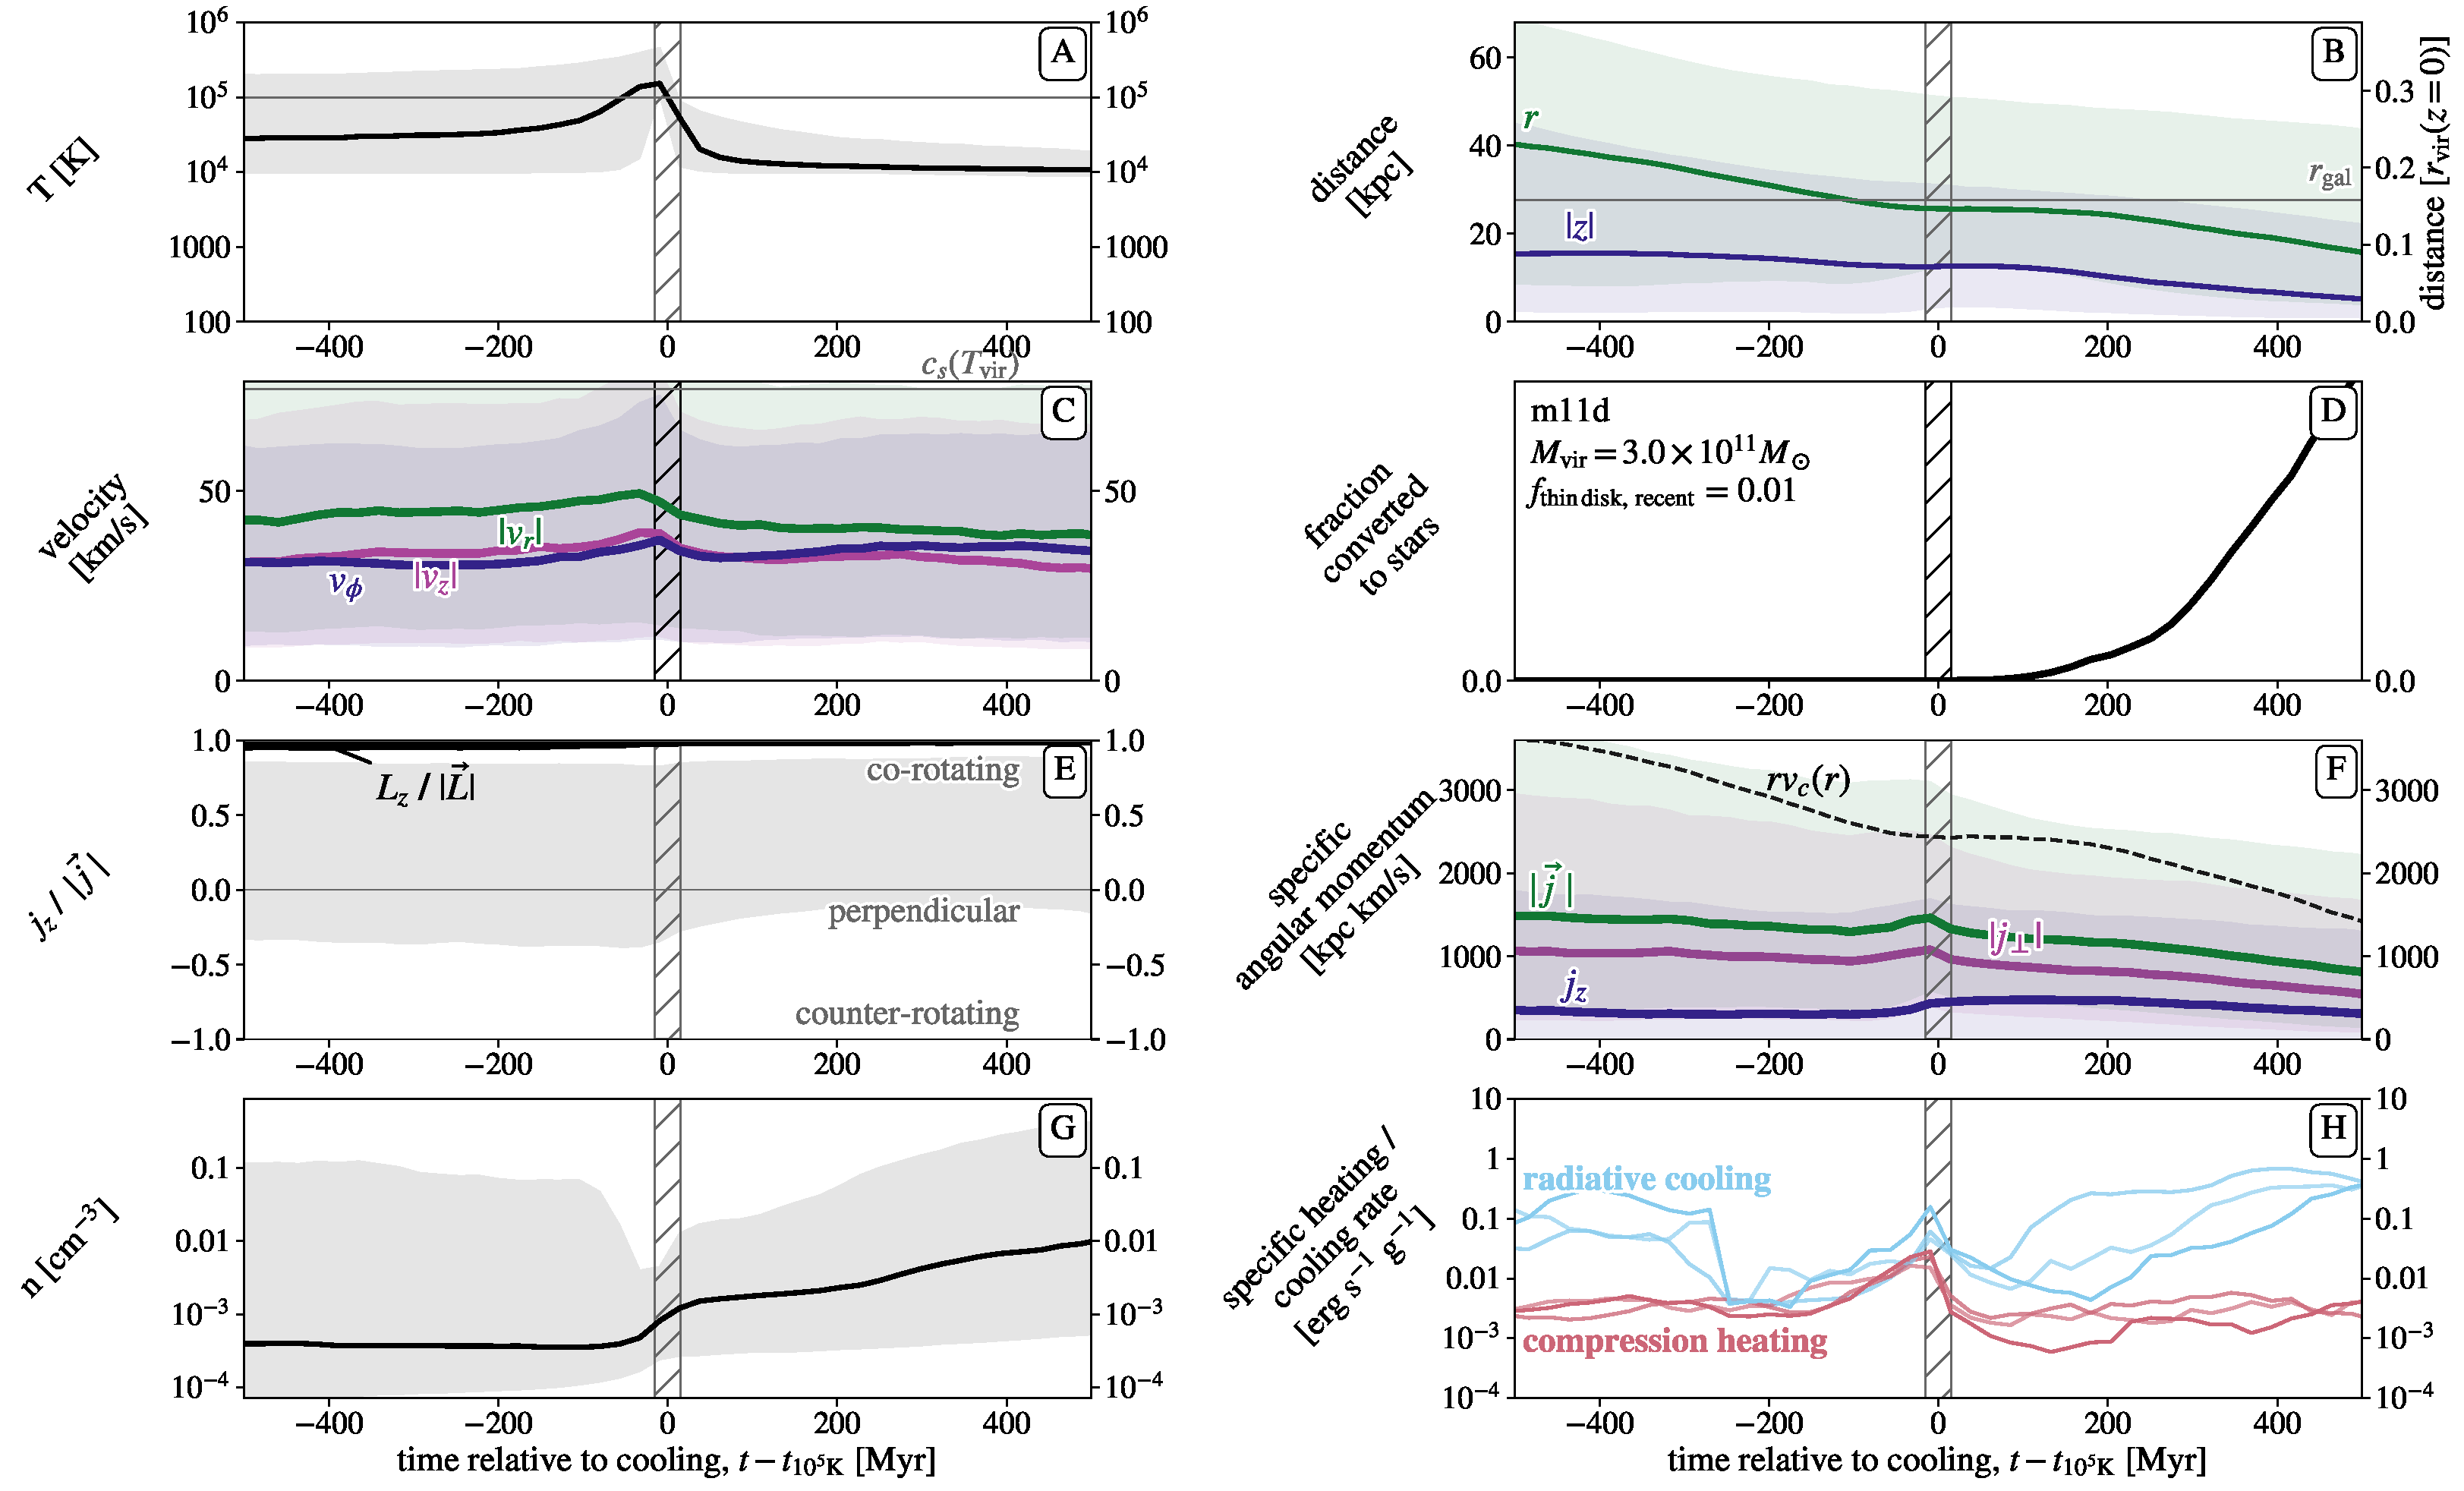
\includegraphics[width=\textwidth]{figures/before_and_after/before_and_after_allone_m11d_md.pdf}
\caption{
Temperature and geometry of gas accreting onto a $z\sim0$ thin disk galaxy in FIRE, versus time relative to the final cooling time ($t - \tcon$).
In each panel solid lines and shaded regions mark the medians and 16th to 84th percentile ranges of all particles accreted within 1 Gyr prior to $z=0$.
\textbf{A:}
Temperature. During the 500 Myr prior to cooling, the inflow is predominantly hot ($\gtrsim 10^5$ K), with a median temperature approaching $\Tvir\approx10^6$ K. At $t = \tcon$ the gas cools to ISM temperatures (by definition).
\textbf{B:}
3D distance from halo center. Prior to cooling the inflow has a typical velocity of $\approx 80$ km s$^{-1}$. Cooling occurs at the galaxy scale $R_{\rm gal}$, after which the inflow stalls.
\textbf{C:}
Absolute height from the disk plane.
Gas collapses into a disk upon cooling, with a median $\vert z \vert \approx 2$ kpc at $t=\tcon$.
% \textbf{E:}
% The magnitude of the specific angular momentum of particles ($\mid\vec{j}\mid$, green) and the component of angular momentum aligned with the galaxy disk ($j_z$; purple).
% The dashed line shows the angular momentum necessary for full rotational support.
% Gas approaches full rotational support immediately before cooling.
}
\label{f: before and after A2}
\end{figure*}



\section{Instantaneous mass flow}
\label{s: appendix-mass flow}

% HOT IN HALO
\begin{figure*}
    \centering
    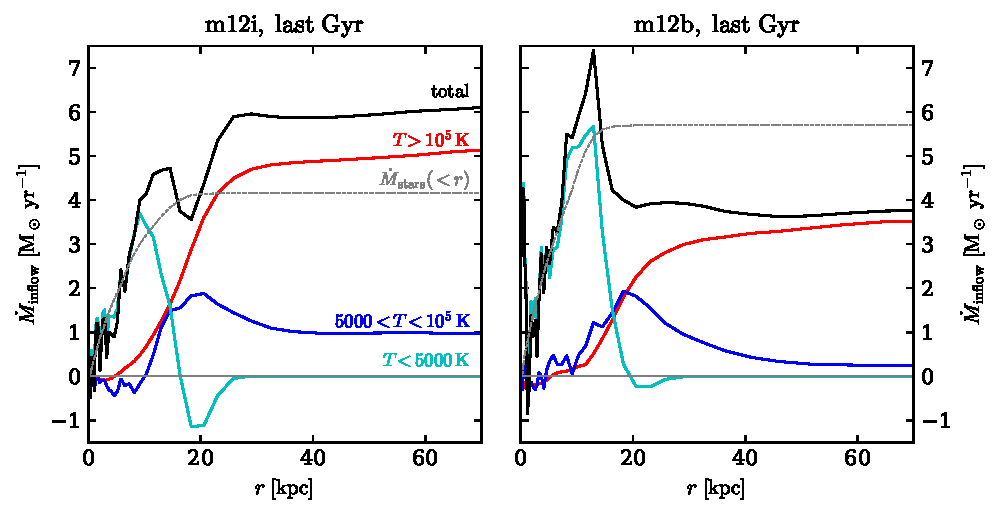
\includegraphics{figures/Mdot.pdf}
    \caption{
    Average mass inflow rate over the course of one Gyr prior to $z=0$ in the same halos as in Figure~\ref{f: stars}, by gas temperature. The galaxy radius $R_{\rm gal}=4 R_{1/2}$ and fraction of stars in a thin disk are marked in the panels. 
    Hot accretion ($T>10^5$ K) dominates the mass inflow onto thin-disk galaxies at $r \gtrsim R_{\rm gal} \sim 10-20$ kpc.
    Cold accretion ($T<10^5$ K) dominates within the galaxy in thin disk galaxies, and in the halo of the lower-mass irregular galaxy shown in the bottom-right panel.
    \textbf{Use consistent capitalization: choose and keep to either R or r.}
    \textbf{Try adding labels relative to $T_{\rm vir}$ (Drummond's suggestion).}
    \textbf{Add ``hot accretion'' and ``cold accretion'' to lines.}
    }
    \label{f: Mdot}
\end{figure*}

We first determine if inflow is dominated by hot or cold gas, which allows us to distinguish a hot inflow from the accretion of cool clouds (formed, e.g., via instabilities).
Figure~\ref{f: Mdot} shows the mass inflow rate versus radius for hot gas (red curves; $T>10^5$ K) and for cool gas (blue curves; $T < 10^5\,{\rm K}$),  for the four simulations shown in Fig.~\ref{f: stars}. 
We calculate the mass inflow rate at a given radius as
\begin{equation}
     \Mdot(r) = \frac{\int_{\rm shell} v_r dm}{\Delta r} = \frac{M_{\rm shell}}{\Delta r} \langle v_r\rangle_{\rm mass\, weighted}
     \label{e: Mdot}
\end{equation}
where $\Delta r=0.05\,{\rm dex}$ is the shell thickness, and the integration is done on all particles with centers within the shell which satisfy the appropriate temperature cut.  We note that the virial temperature of the four halos is $\Tvir = xx, yy, zz$ and $ww$ K, so in all cases we expect an $\sim\Tvir$ inflow  to be considered `hot'. 

% Consequences
In the three MW mass galaxies with a large thin disk fraction, at halo scales of $r>20$ kpc the inflow is dominated by hot gas, where in m12i and m12b $\Mdot$ of the hot gas is larger by a factor of $\gtrsim 4\times$ than that of cool gas. The greater mass flux of hot gas indicates that the dominant form of accretion is an inflowing hot phase, rather than cold flows or cool clouds precipitating from the hot phase.
In contrast, in the lower mass galaxy shown in the bottom right the inflow is dominated by cool gas, while the hot gas is outflowing out to $\approx50$ kpc.

Fig.~\ref{f: Mdot} also shows that the inflow rate of hot gas in the MW-mass galaxies drops within $R_{\rm gal}$, reflecting the cooling of the hot inflow at the galaxy-halo interface, as shown in the next section.


\section{Notes on individual galaxies}

\label{s: appendix-individual}

% Presence of a rotating cooling flow for intermediate cases
The halos with $0.1 < f_{\rm thin\,disk,\,recent} < 0.5$ have varying levels of circularized cooling flow accretion.
Three of these four halos, \texttt{m12r} and \texttt{m12w}, have $M_{\rm vir} \sim 10^{12} M_\odot$.
\texttt{m12r} has some ongoing thin disk formation, but is undergoing a major merger during the last Gyr that dominates the accreting gas supply and disrupts the galaxy structure.
This merger is relatively well-aligned with the disk, with $f_{\rm aligned} \approx 0.3-0.4$, and the aligned mass fraction does not change significantly as the gas cools past $\tcon$.
\texttt{m12w} is a galaxy with its inner CGM is only just virializing at $z=0$~\citep{Yu2021}, and the majority of the gas accretes with angular momentum perpendicular to the galaxy angular momentum.
The third halo, \texttt{m12m}, is galaxy undergoing significant rotating cooling flow accretion, but absent a high thin disk fraction.
Visual inspection reveals that \texttt{m12m} has a prominent stellar bar.
\texttt{m12m} may be evidence that if rotating cooling flows are a condition for disk formation, they are a necessary-but-not-sufficient condition (\S\ref{s: disk formation -- condition}).
\texttt{m12m} is one of the few MW-mass halos that does not include metal diffusion, which may play a role in its morphology.
The fourth halo is \texttt{m11h}, a galaxy that is beginning to form a disk despite its virial mass of $M_{\rm vir}(z=0) \approx 2 \times 10^{11} M_\odot$.
Much of its accretion is still isotropic, but there is increased alignment post-cooling.



% \section{Analysis for a halo with cosmic ray feedback}
% \label{s: appendix-crs}

% % MECHANICS OF ACCRETION
% \begin{figure*}
% 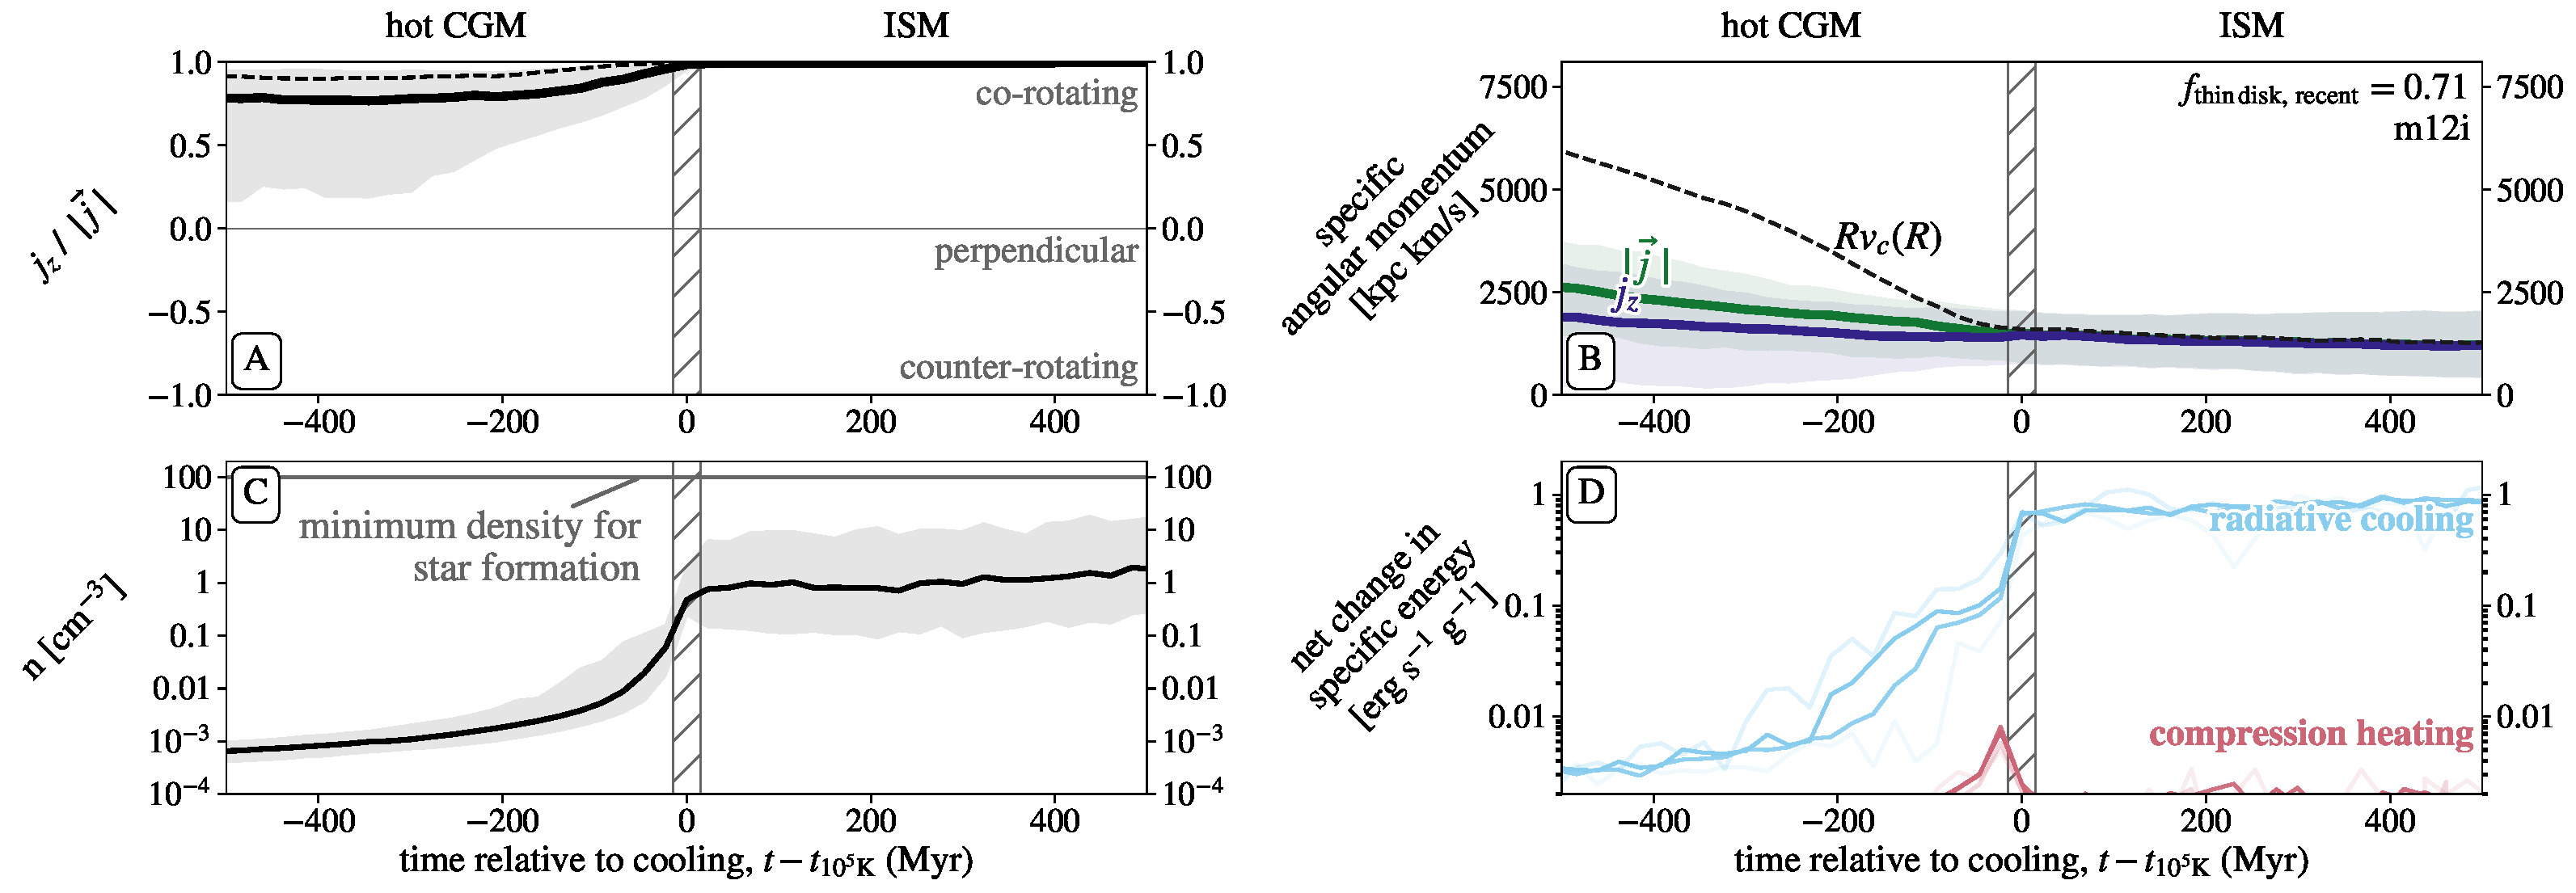
\includegraphics[width=\textwidth]{figures/before_and_after/before_and_after_m12i_cr.pdf}
% \caption{
% Same as Figure~\ref{f: before and after} but for \texttt{m12i} evolved with cosmic ray feedback.
% Despite having nonthermal feedback, the characteristics and mechanics of accretion are qualitatively and quantitatively very similar to thin-disk galaxies without cosmic ray feedback.
% }
% \label{f: before and after -- cr}
% \end{figure*}

% % Summary
% Figure~\ref{f: before and after -- cr} shows the mechanics of accretion for a halo with cosmic ray feedback, \texttt{m12i\_cr}.

% \section{Angular Momentum of Accreting Material}

% \begin{figure}
%     \centering
%     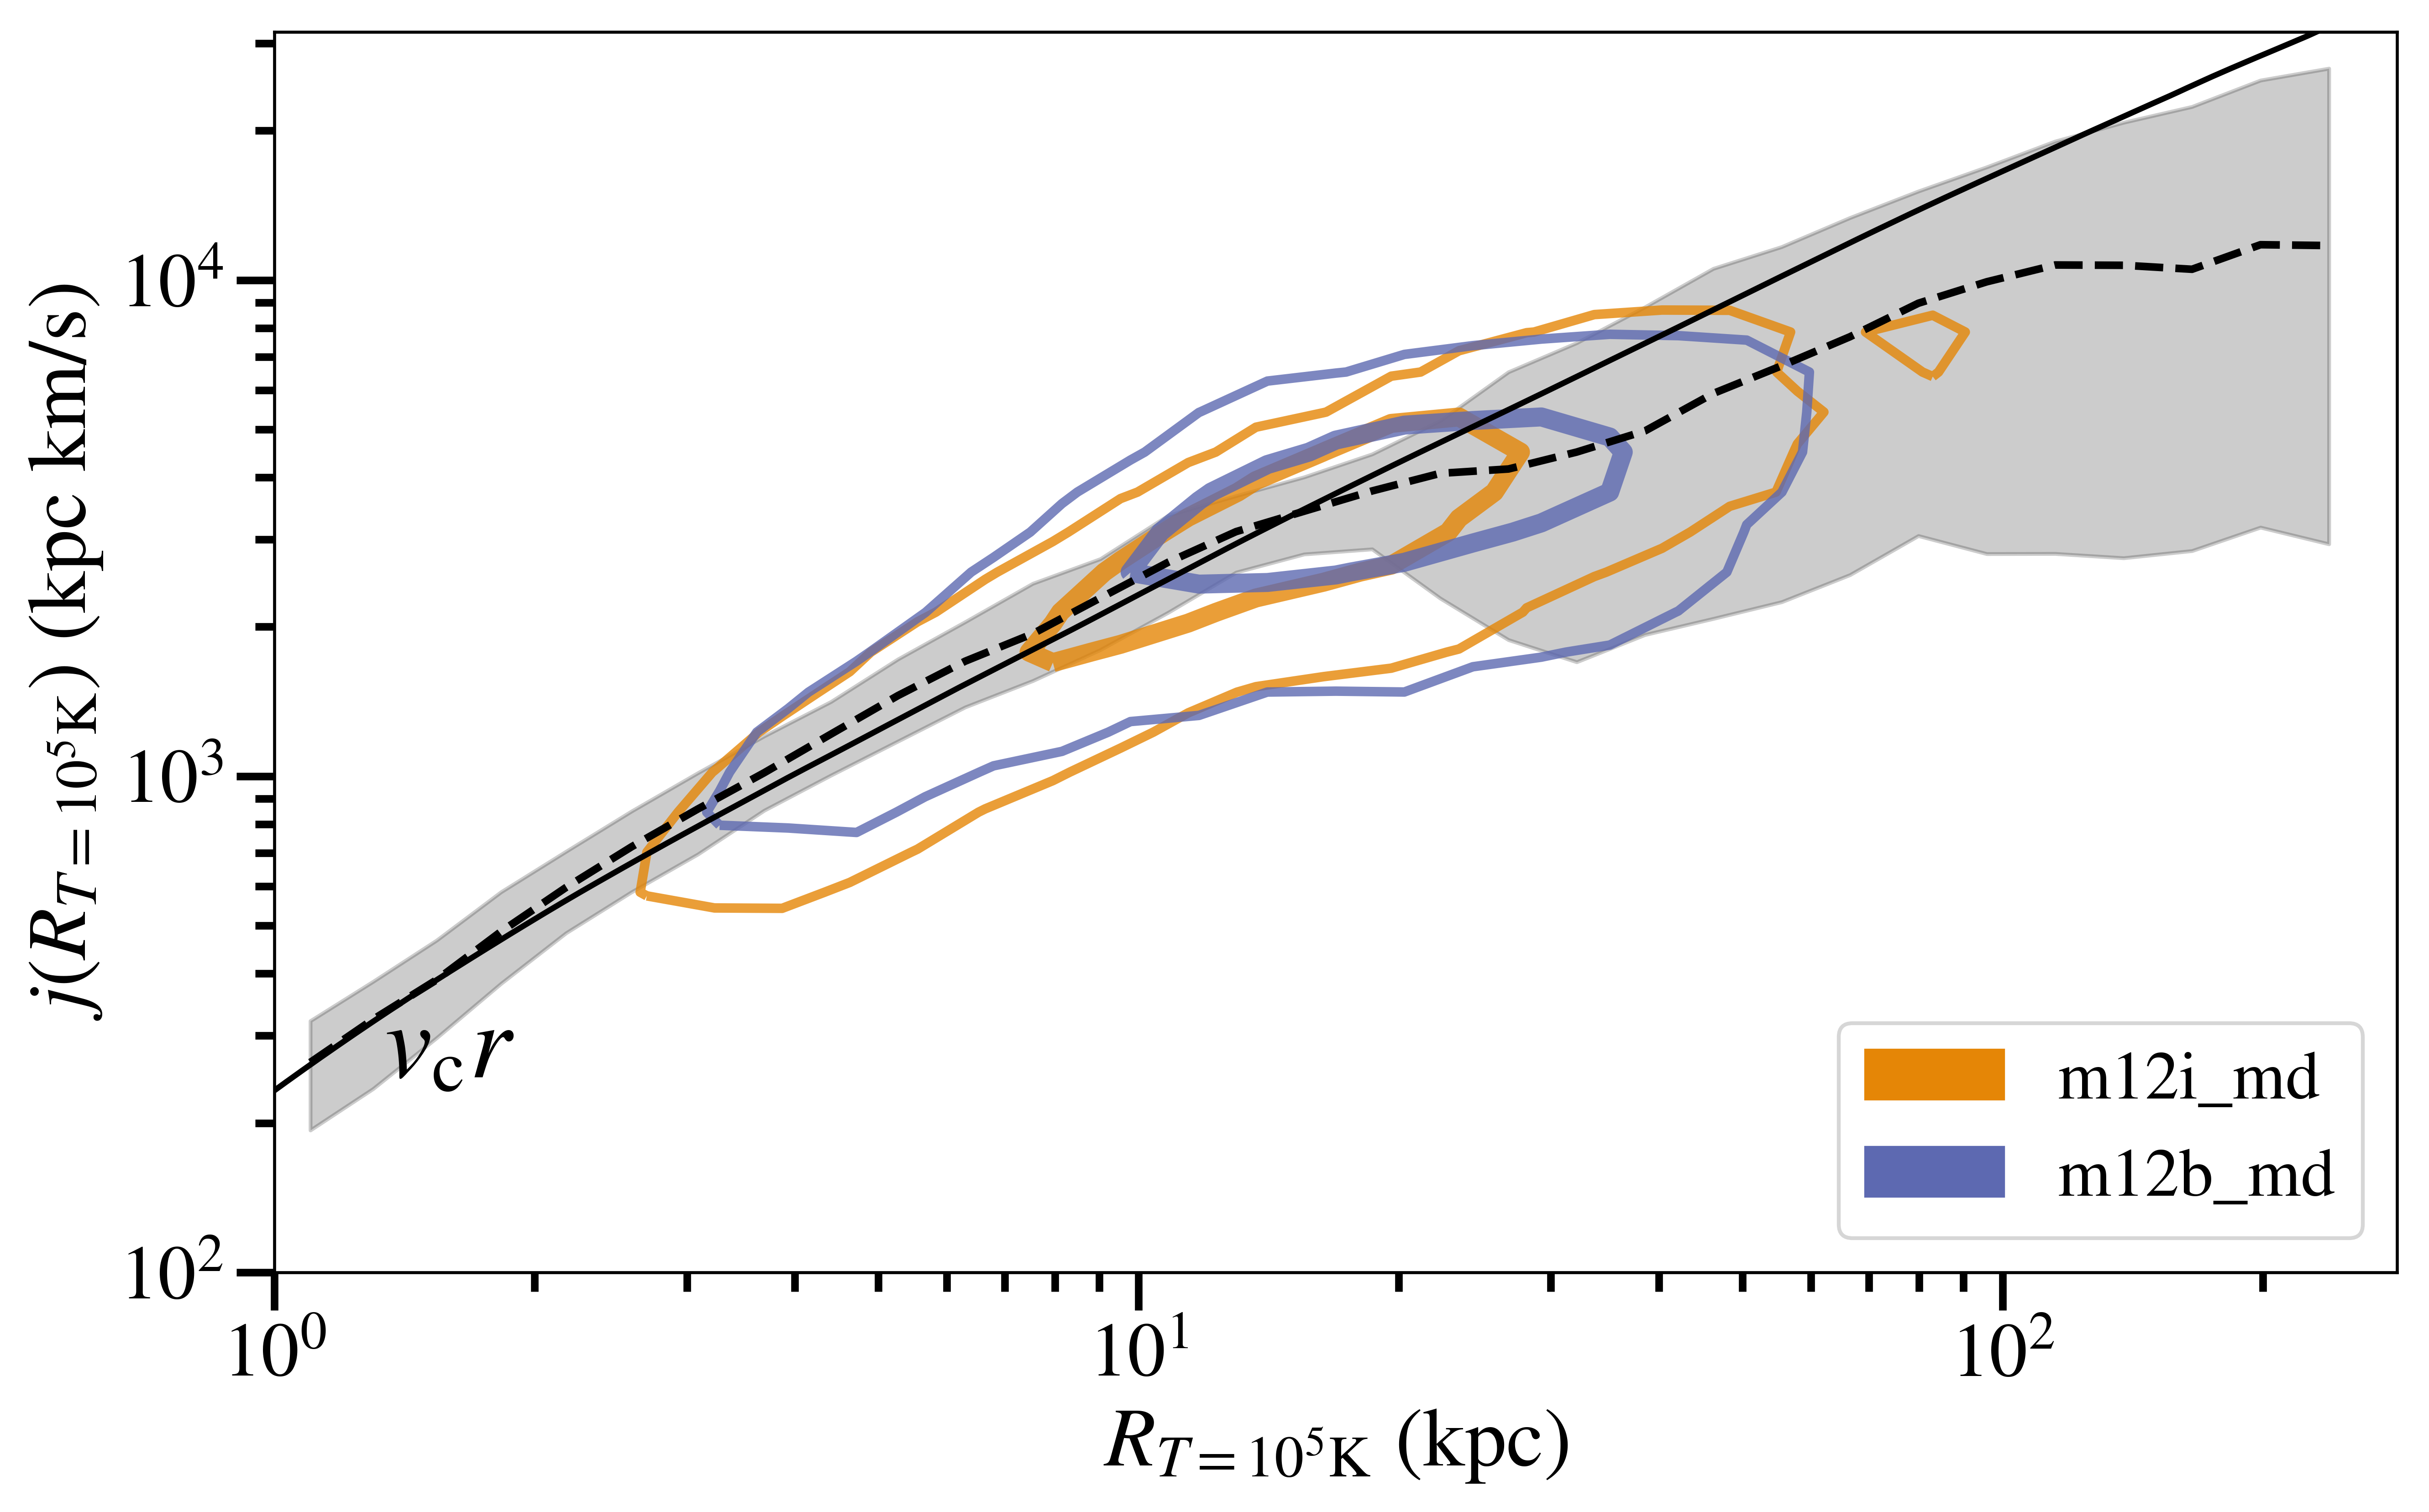
\includegraphics[width=\columnwidth]{figures/j_vs_rcondense.png}
%     \caption{
%     Distribution of $\Rcon$ vs j($\Rcon$) for four FIRE-2 halos with $L(z=0) \sim L^\star$.
% Thick (thin) contours enclose values for 50\% (90\%) of the accreted gas particles.
% The angular momentum as a function of radius for all gas in \texttt{m12i} at $z=0$ is displayed as a dashed line (the median) and shaded regions (5th-95th percentiles).
% \textbf{
% Maybe delete this figure later, because it's only relevant for simulations that have a wide distribution of $\Rcon$, which are only the artificially wide non-md runs.
% }
% \textbf{Is the 100 kpc-cooling gas related to satellite galaxies?}
% \textbf{Try changing shaded region to only hot gas instead of all gas.}
% \textbf{Try histogram of r/(j/vc) instead, to demonstrate that that decreases the spread.}
% \textit{
% In all halos the distributions are consistent with $j_{\rm c} = v_{\rm c} r$, i.e. gas cools once circularized.
% This demonstrates that the variable angular momentum of incoming gas drives the width in the $\Rcon$ distribution.
% }
%     }
%     \label{f: jcool vs Rcon}
% \end{figure}

%%%%%%%%%%%%%%%%%%%%%%%%%%%%%%%%%%%%%%%%%%%%%%%%%%


% Don't change these lines
\bsp	% typesetting comment
\label{lastpage}
\end{document}

% End of mnras_template.tex
